\documentclass[a4paper]{article}
\usepackage{bm} 
%boldmaths fonts, no interrupting the spaceshttps://www.sharelatex.com/project/551e9dc5a9905cd2390a7fda
\usepackage{sidecap}
\usepackage{tabularx}
\usepackage[margin=0.5in]{geometry}
\usepackage{color}
\usepackage{caption}
\newcommand{\YWG}[1]{\noindent \color{blue} #1 \normalcolor}


\usepackage{graphicx}
\usepackage{sectsty}
\sectionfont{\fontsize{14.4}{18}\selectfont}
\subsectionfont{\fontsize{14}{17}\selectfont}
\subsectionfont{\fontsize{12}{14.4}\selectfont}

\title{\textbf{ 
    \Large {Operation Manual for} \\ 
    \vspace {10pt}
    \Huge {P$\bm{\mu}$SL 3D-Printer } \\
    \vspace {10pt}
    \LARGE {in precision mode}	\\
    \vspace {10pt}
    \Large{(McKay 304)}
    \vspace {20pt}
}}
\author{\textit{Tianyu Gu} \\
  \textit{Yiwei Guo}\\
  \textit{Sicong Shan}\\
  \textit{Bertoldi Group}}
\date{\today}

\begin{document}

\maketitle
\vspace{50pt}
\centering
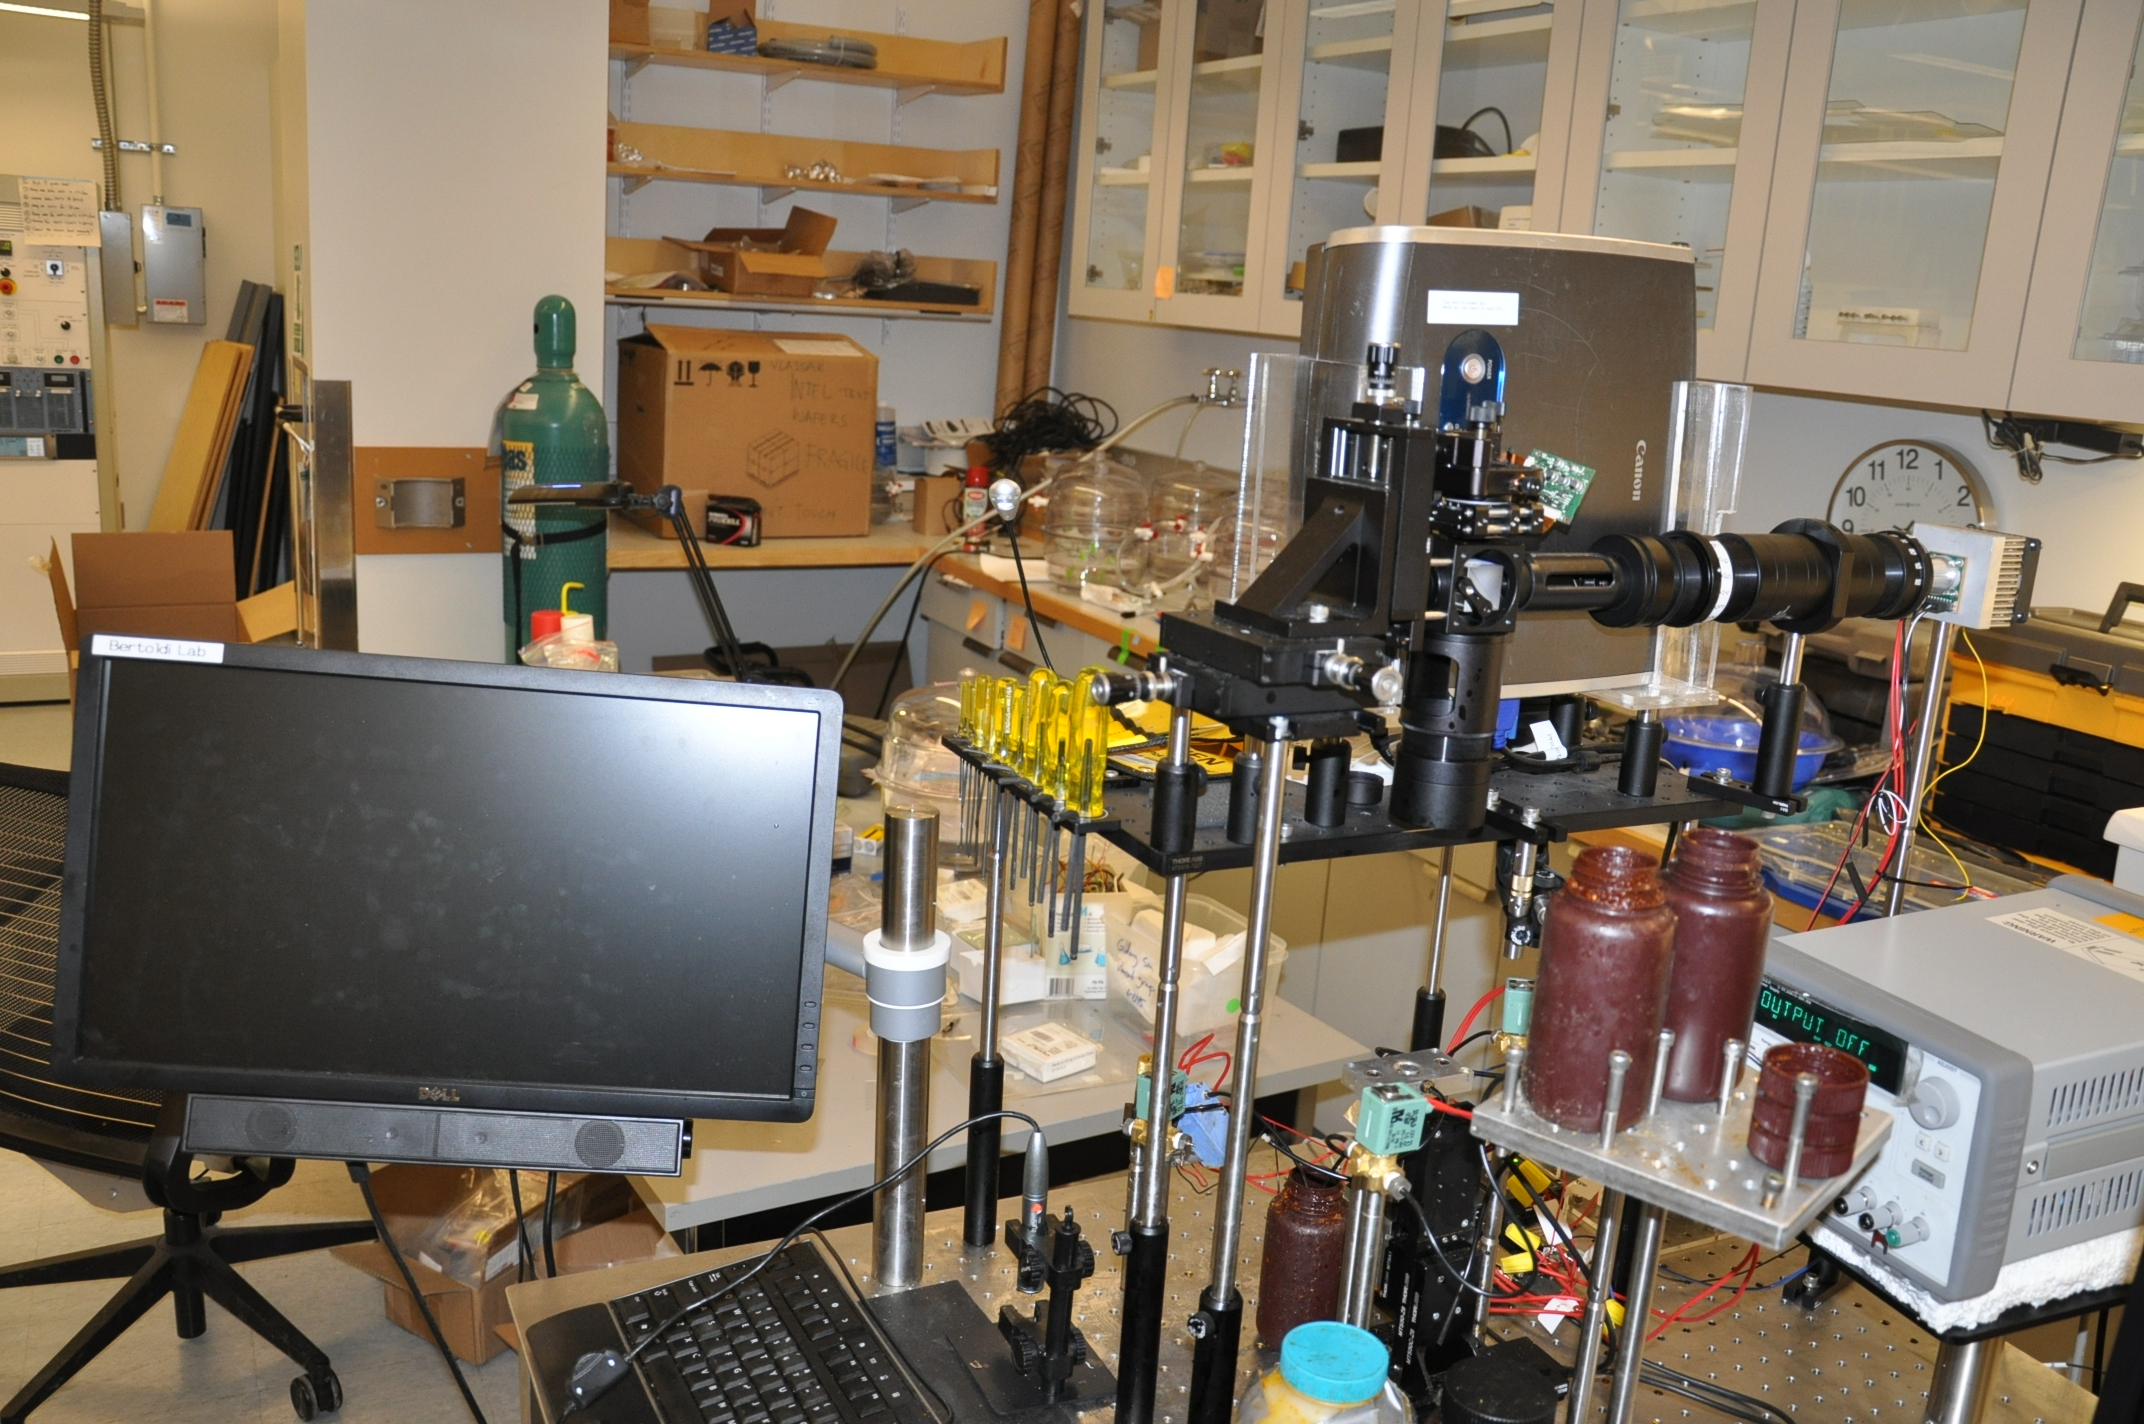
\includegraphics[width=400pt]{mainoverview.JPG}
\pagebreak

\tableofcontents
\pagebreak

\raggedright
\section{System introduction}
Projection micro-stereolithography (P$\mu$SL) offers unique opportunities to incorporate various material systems into
micro structures and micro devices to achieve exceptional functionality. Also due to the freedom of manufacturing 
three-dimensional architectures at micron scale, P$\mu$SL makes it possible to fabricate sophisticated strutures with 
complex geometries and dimensions.With the help of P$\mu$SL, many designs and inspirations which could not be rapidly 
realized otherwise can be easily explored and investigated.  \\
\vspace{20pt}
P$\mu$SL is a novel 3D microfabrication technique capable of making highly complex 3D micro structures in an additive, 
layer-by-layer fashion with micro scale resolution. P$\mu$SL utilizes the most advanced digital micro display technology, 
a liquid crystal on silicon (LCOS) chip , as a dynamic mask generator, to function as a virtual photomasks capable of 
producing digitally and dynamically configured patterns.The illustration of the P$\mu$SL system was shown in the picture 
below.\footnote{Howon Lee,THREE-DIMENSIONAL MICRO FABRICATION OF ACTIVE MICRO DEVICES USING SOFT FUNCTIONAL MATERIALS
  ,P10}\\
\vspace{20pt}
\centering
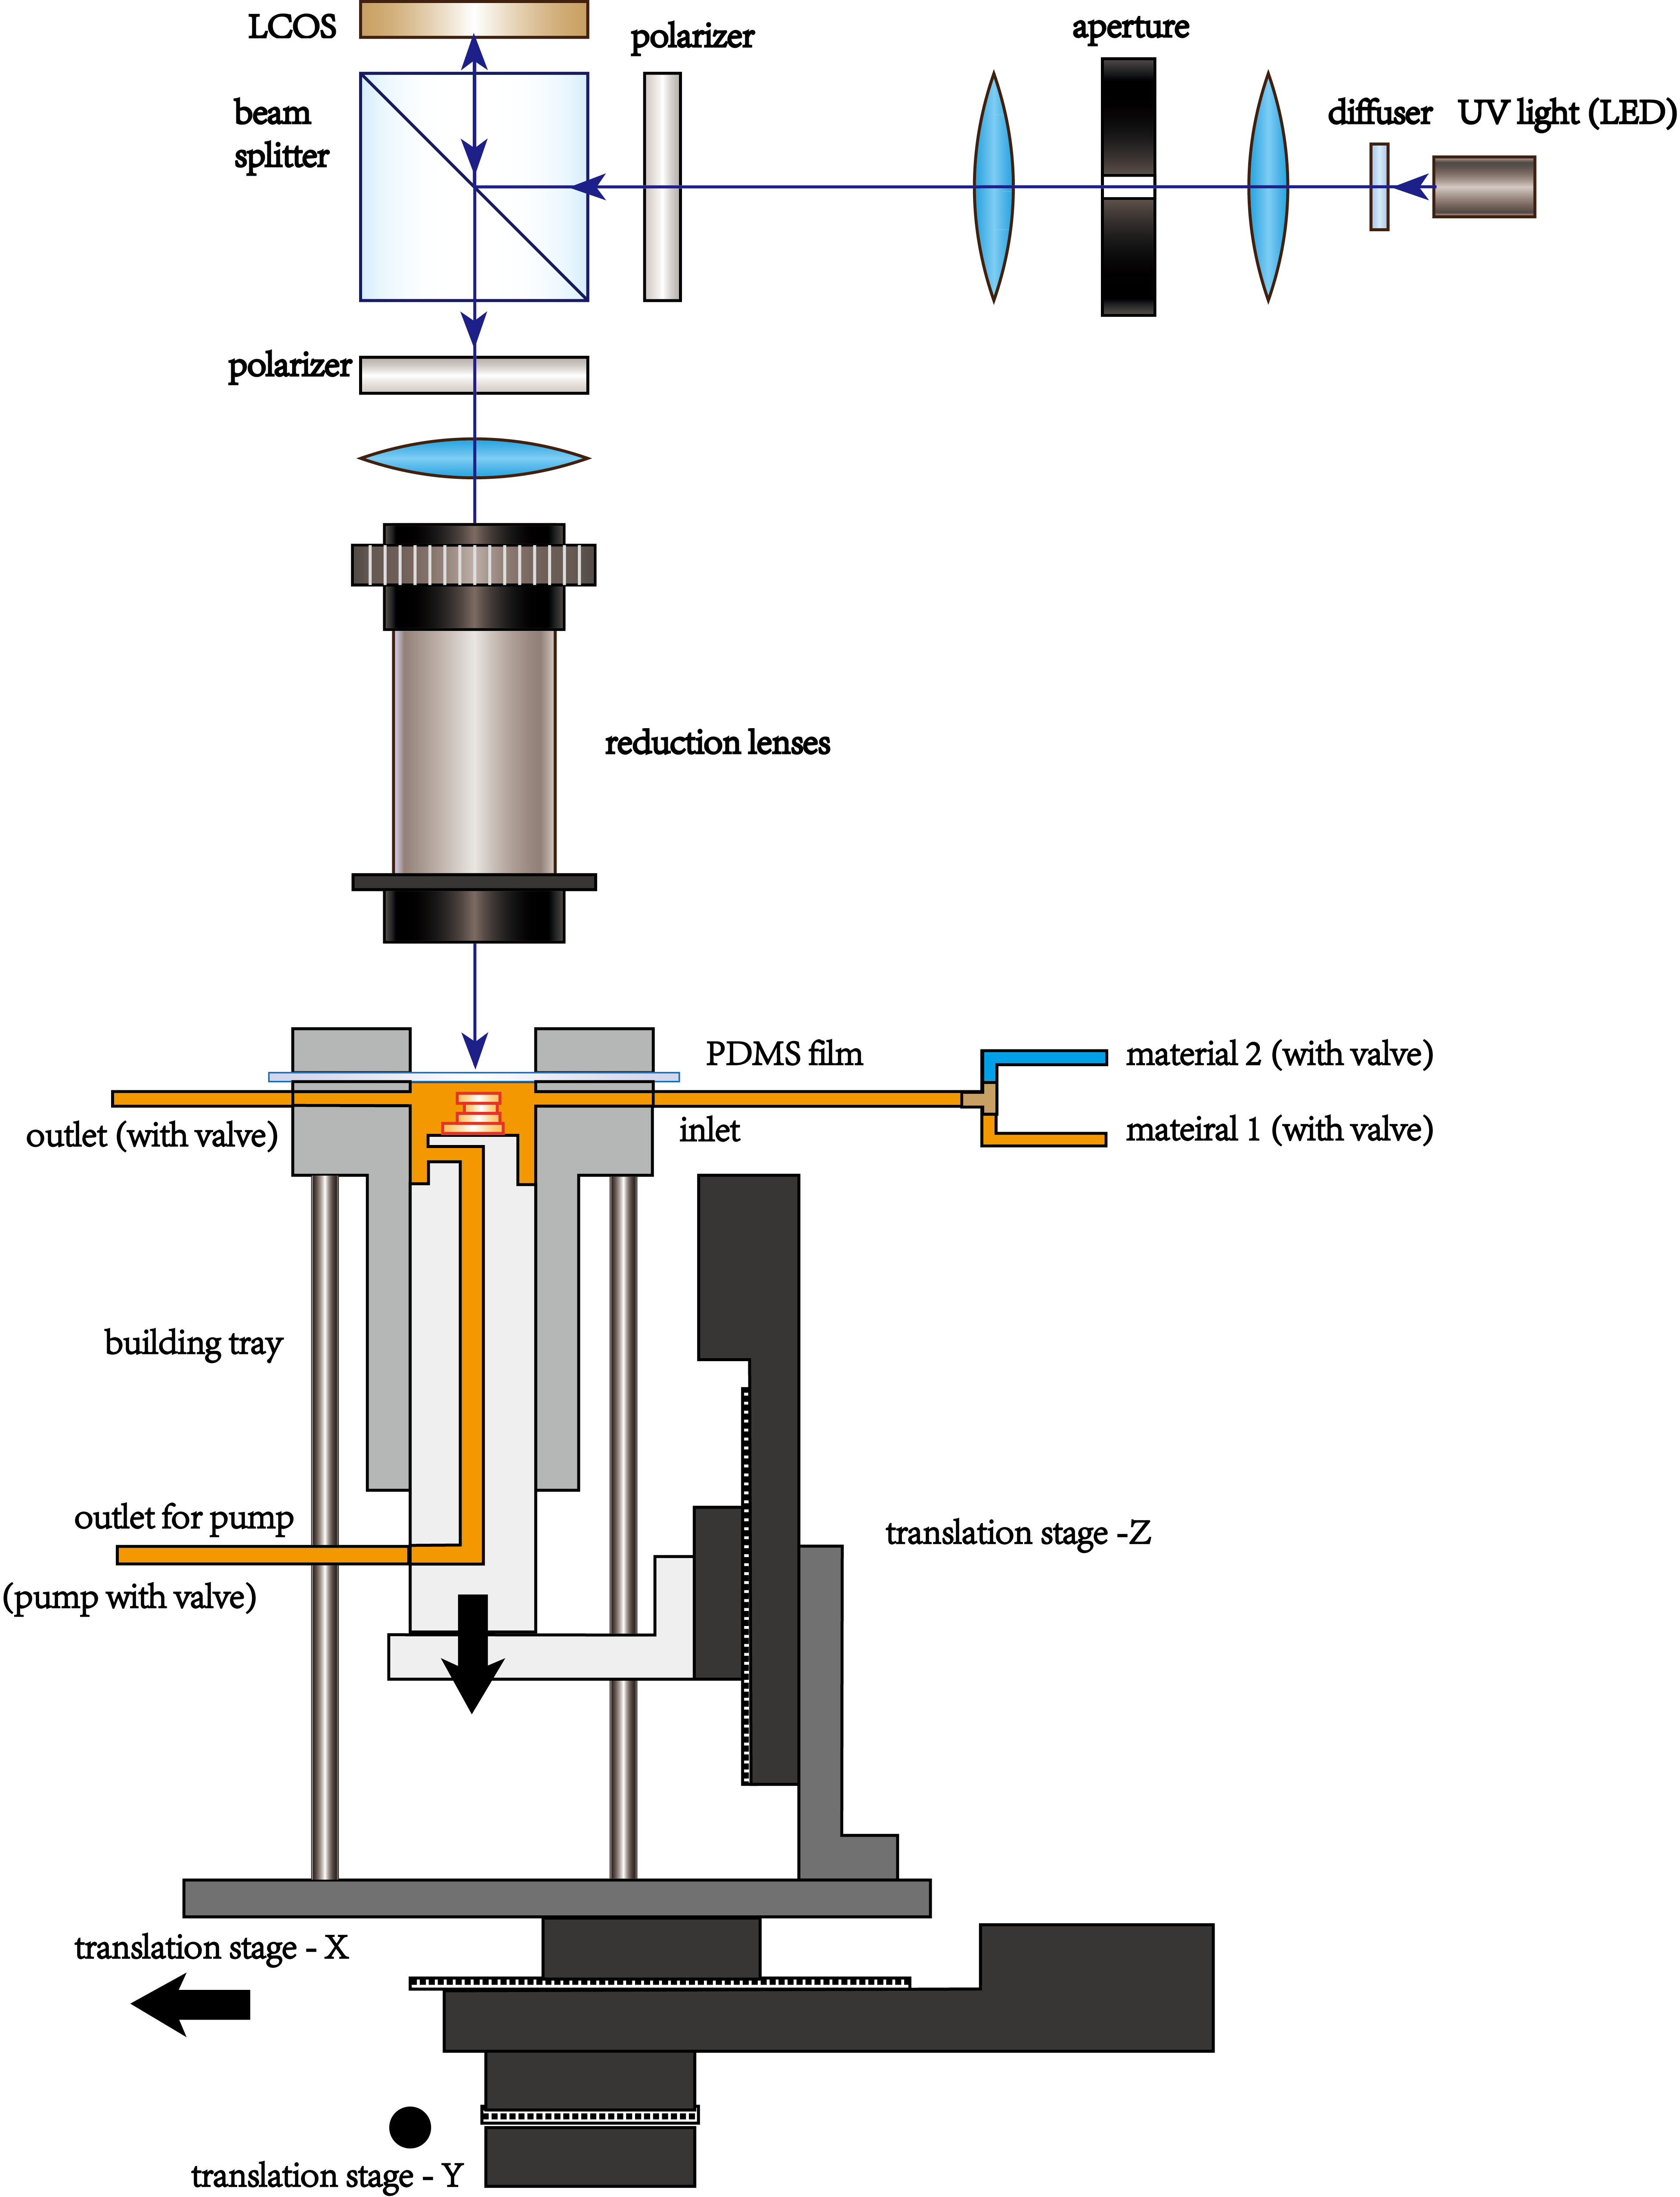
\includegraphics[width=400pt]{overview.png}\\
\textit{the illustration of the P$\mu$SL system}
\vspace{20pt}
\pagebreak

\raggedright

\underline{All the actions are set to BOLD and all equipments are in italics. The underlined part should be paid attention!} 
\subsection{Hardware}
\subsubsection{List of the hardware}
\begin{table}
  \begin{center}
    \begin{tabular}{|c | c | c | c | c |}
      \hline
      \textbf{Number}\textbf{name}&\textbf{company}&\textbf{catalog number}&\textbf{comments} \\ 
      \hline
      1 & Projector & Canon & REALIS SX-50 & LCOS \\ 
      \hline
      2 & UV LED & Innovations in optics & 2600N-700 & 365nm~405nm wavelength \\     
      \hline
      3 & Pump & Parker & L.3M06E2.A12VDC & LTC Diaphragm Pump \\ 
      \hline
      4 & Motorized stage & Thors Lab & MTS50-Z8 & Linear stage \\ 
      \hline
      5 & Stage controller & ThorsLab & TDC-001 & To control the stage movement \\ 
      \hline
      6 & Powersupply & Agilent & E3633A & Power UV LED and valves \\      
      \hline
      7 & Electronic microscope & Supereye & A005+ & For microscopic observation \\ 
      \hline
      8 & Printing chamber & Machine shop & none & Customer-made \\ 
      \hline
    \end{tabular}
  \end{center}
  \caption{The purchasing list of the hardware}
\end{table}

\subsubsection{LCOS chip(Projector)}
\textit{LCOS chip}, which stands for \underline{liquid crystal on silicon}\footnote{The underlined part should be 
  paid attention!}, is the core part in both the projectors and the whole system. It can dynamically generate digital-masks 
and reflect the flood of Ultra-violet light into desired projection image. 
\begin{tabularx}{\textwidth}{ XXX} 
  \raisebox{-\height}{\includegraphics[width=0.3\textwidth]{Lcos.jpg}}
  &\raisebox{-\height}{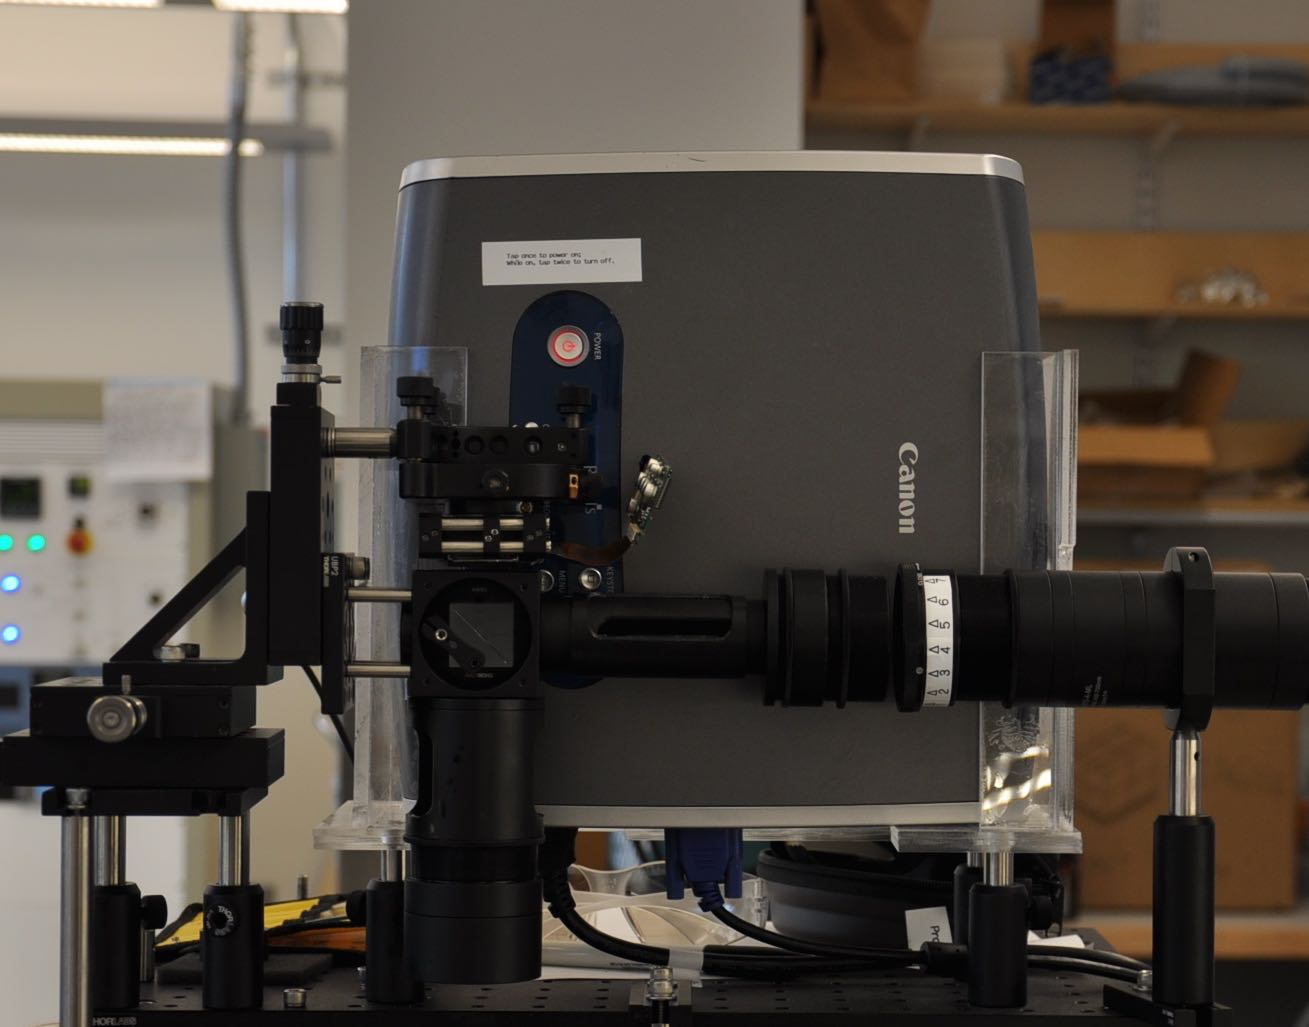
\includegraphics[width=0.3\textwidth]{projectorinsystem.jpg}}
  &\raisebox{-\height}{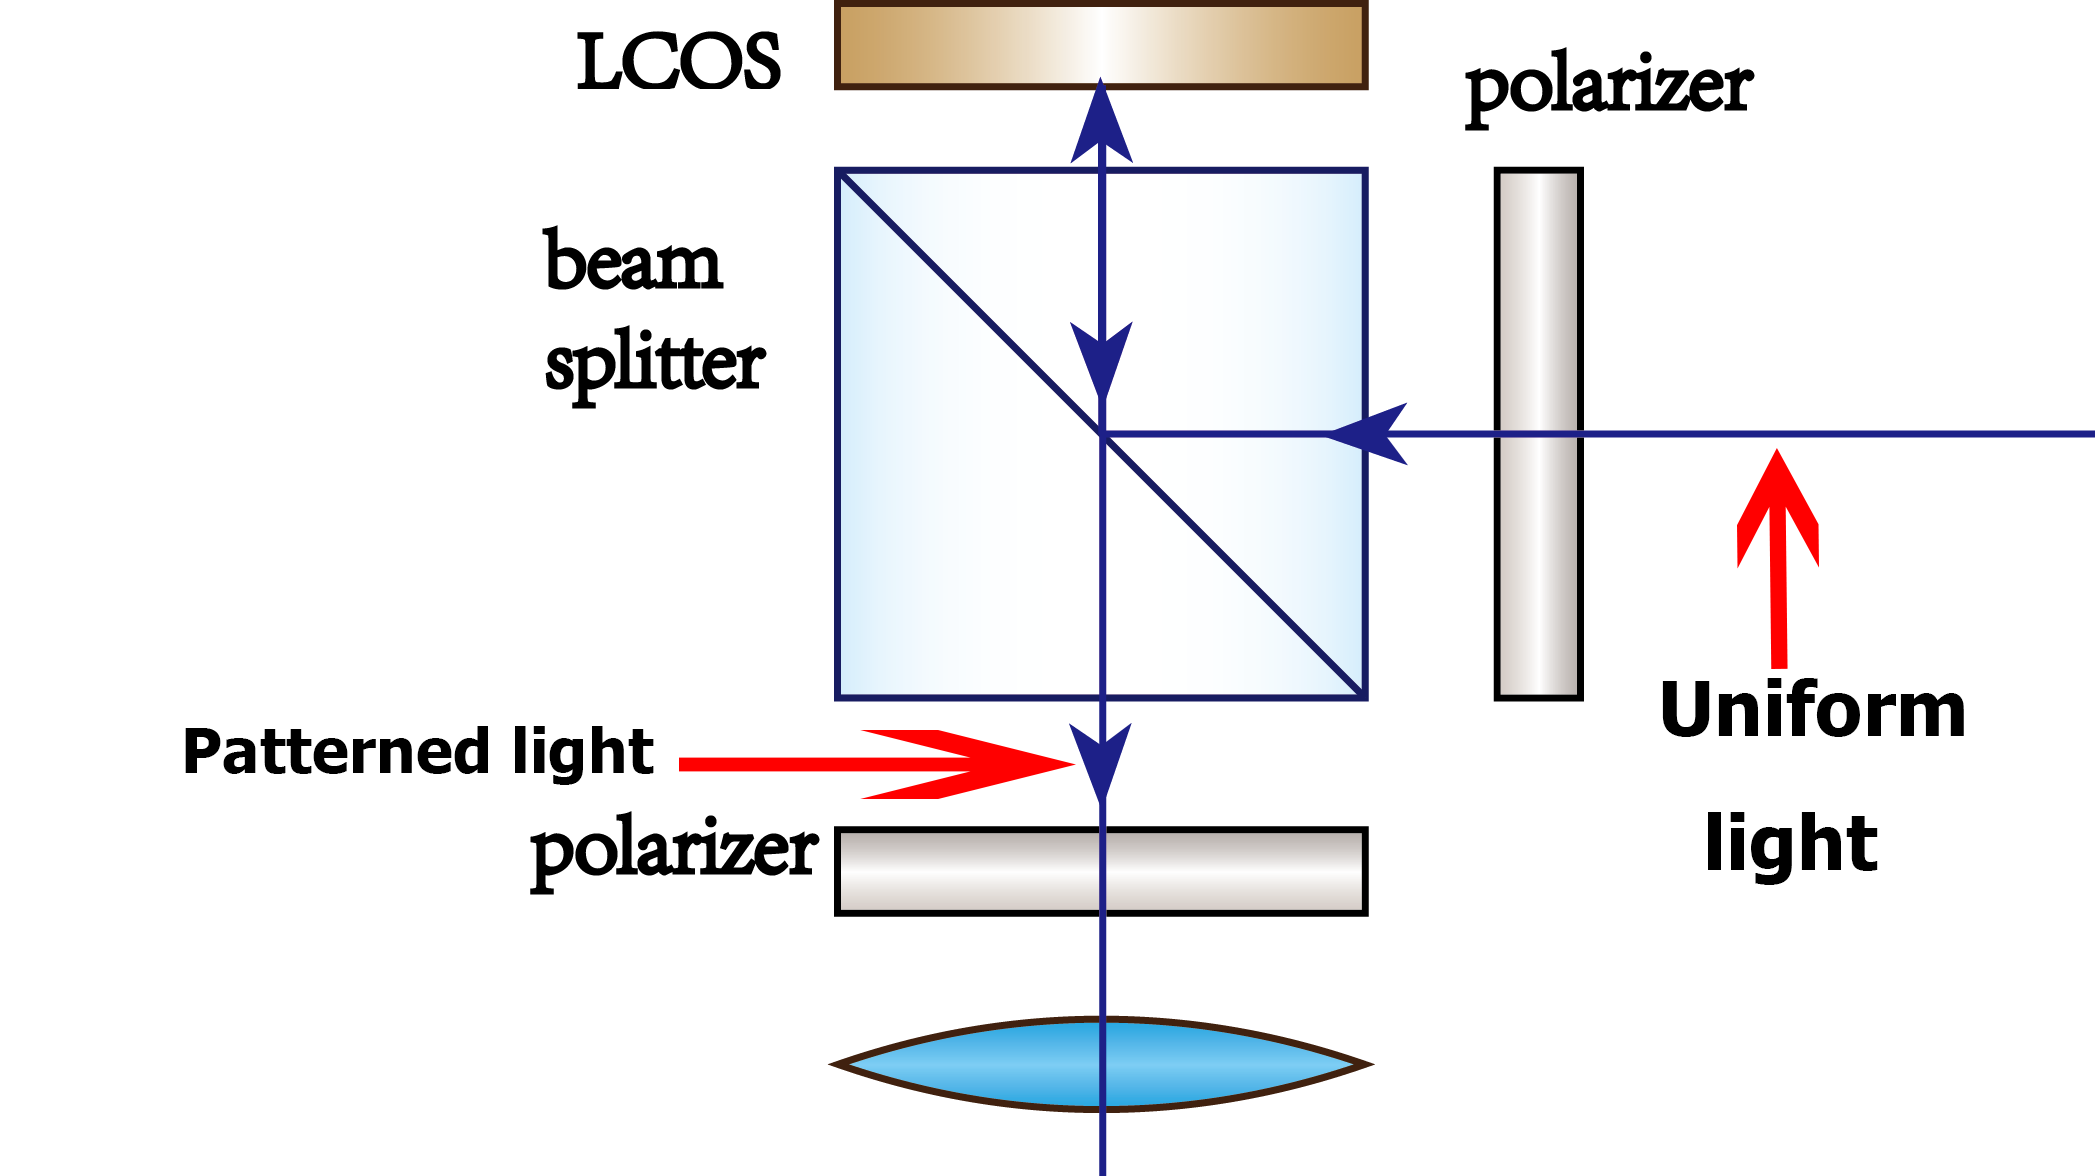
\includegraphics[width=0.3\textwidth]{overview1.png}}
  \\
\end{tabularx}

\subsubsection{UV LED source}
\textit{UV LED} source generates 405nm wavelength Ultra-violet light which is capable of curing the prepolymer solution. 
\textit{Fans} are installed right behind the light source to ensure that the intense heat generated by the \textit{UV LED} 
could be dissipated into the air.
\begin{tabularx}{\textwidth}{ XXX} 
  \raisebox{-\height}{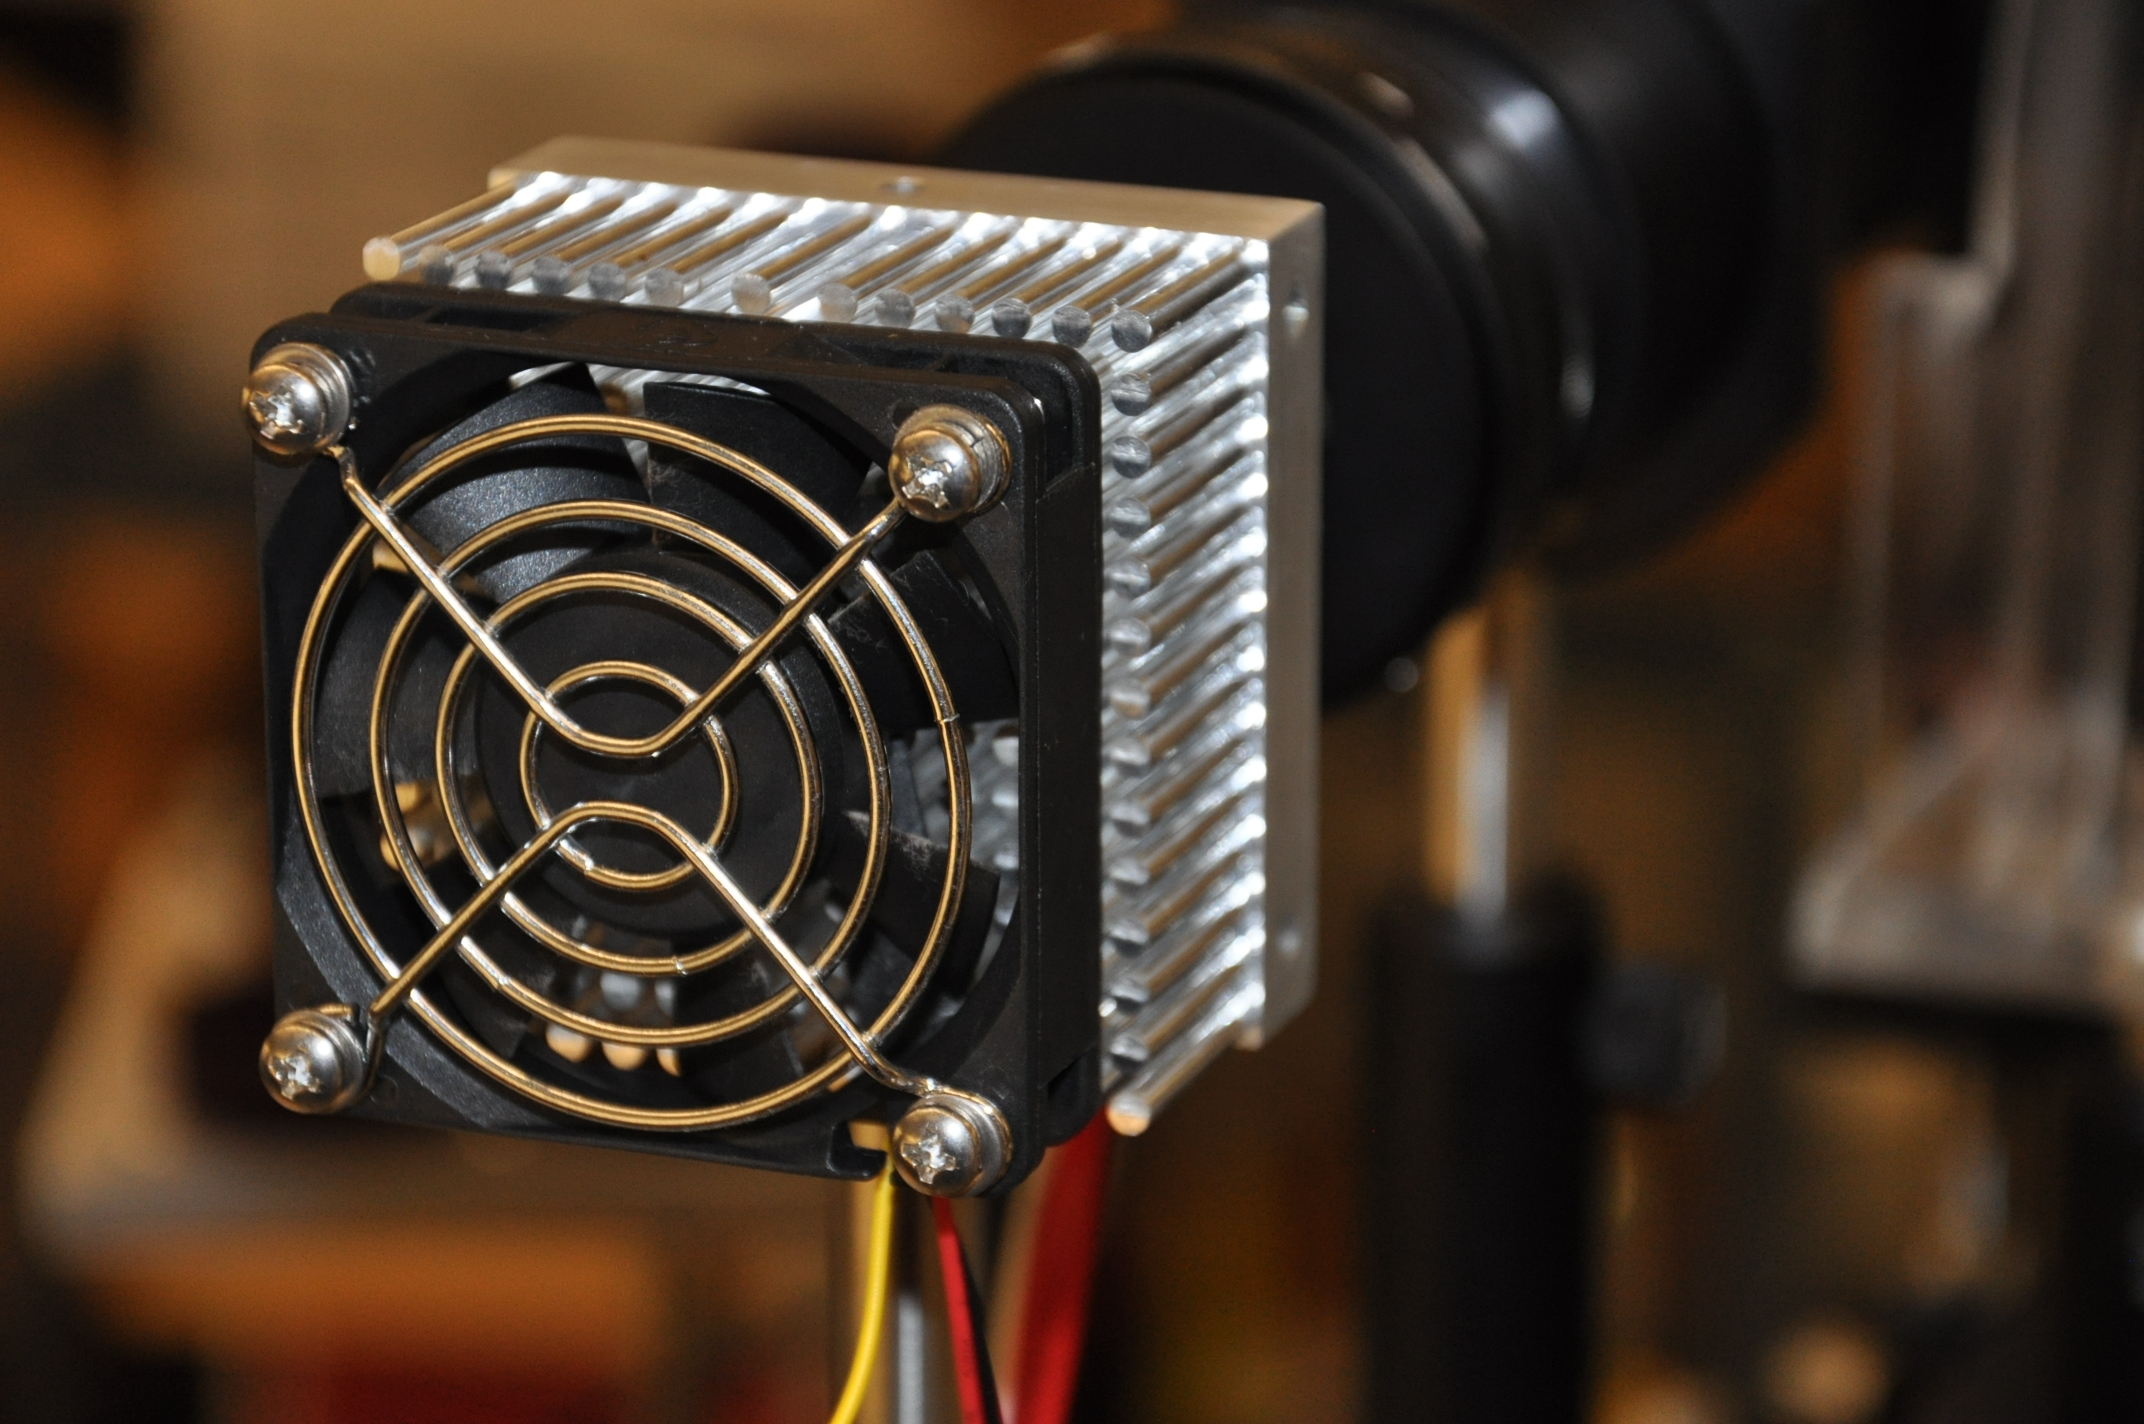
\includegraphics[width=0.3\textwidth]{step_1_fan.JPG}}
  &\raisebox{-\height}{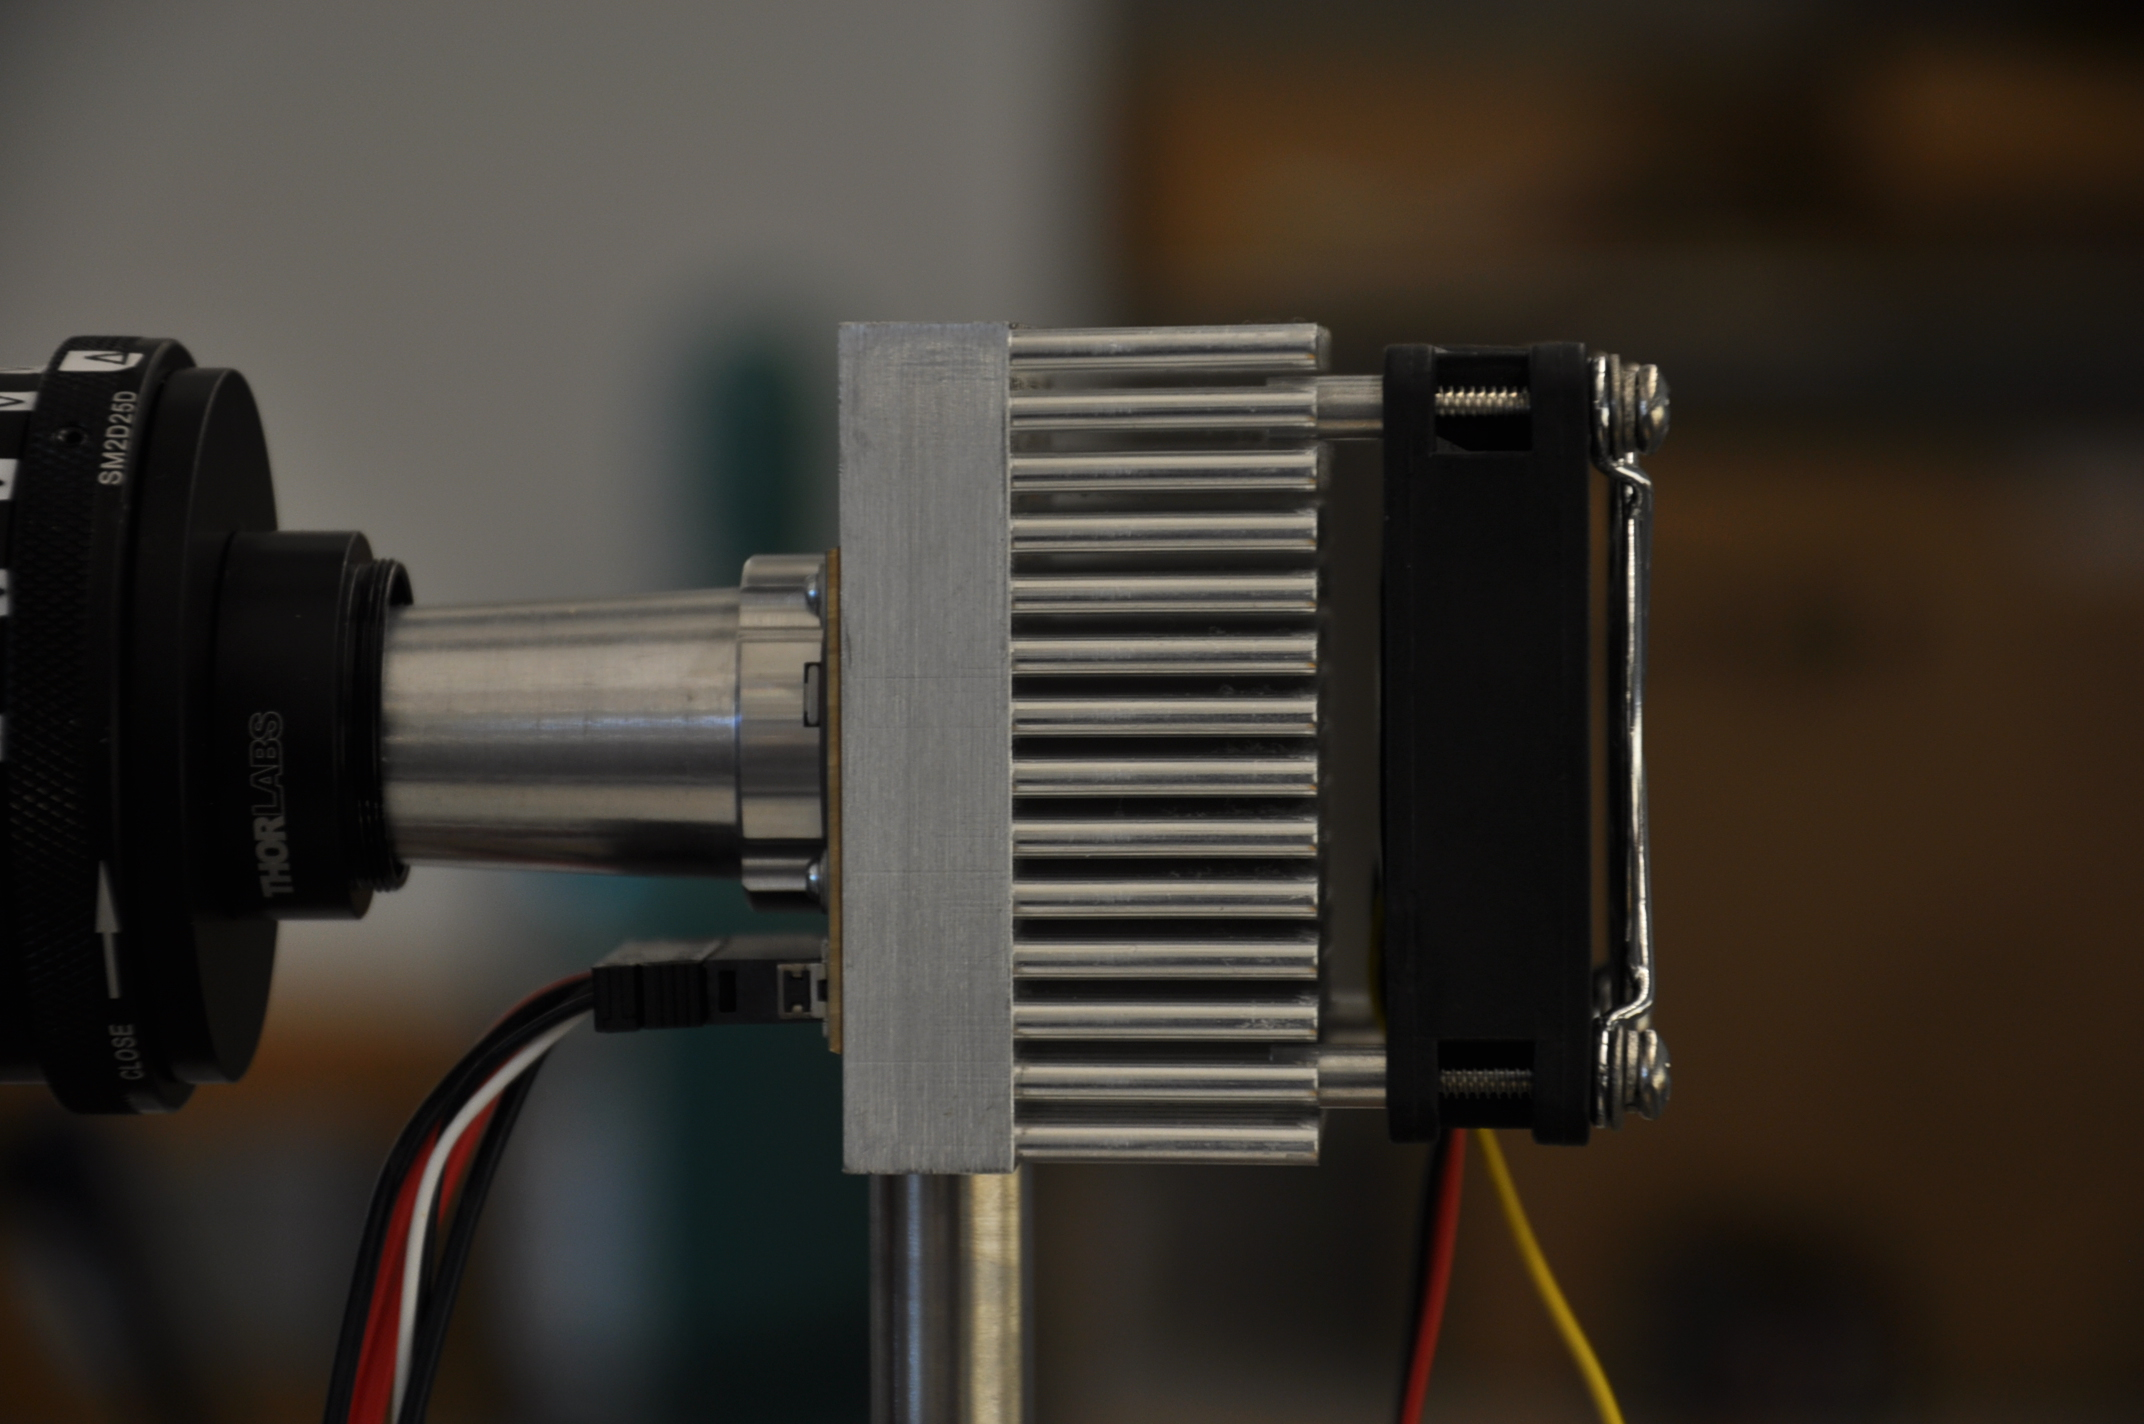
\includegraphics[width=0.3\textwidth]{uvlightfan.JPG}}
  &\raisebox{-\height}{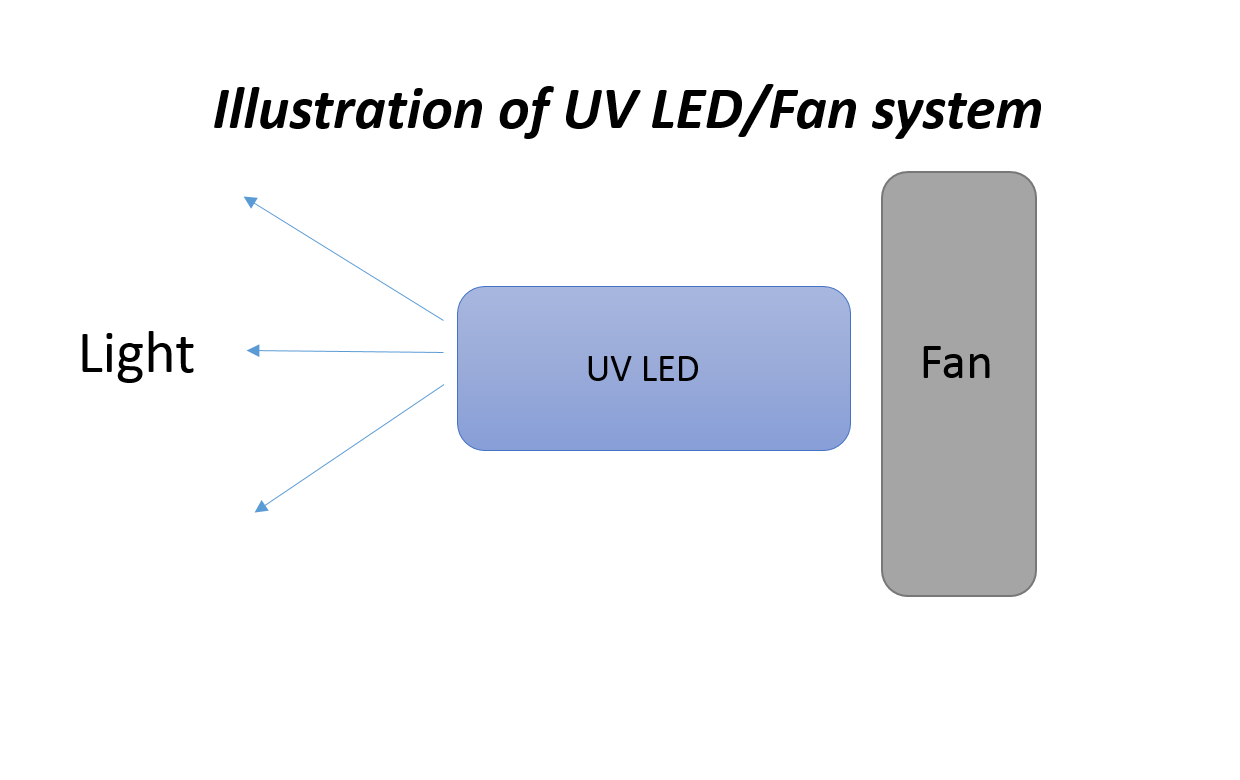
\includegraphics[width=0.3\textwidth]{uvfanil.PNG}}
  \\
\end{tabularx}

\subsubsection{Optical system}
The optical system consists of the convex lens, polarizing beam splitter and reduction lens. See figure 
\ref{figure_optical_path}.
\begin{figure}
  \centering
  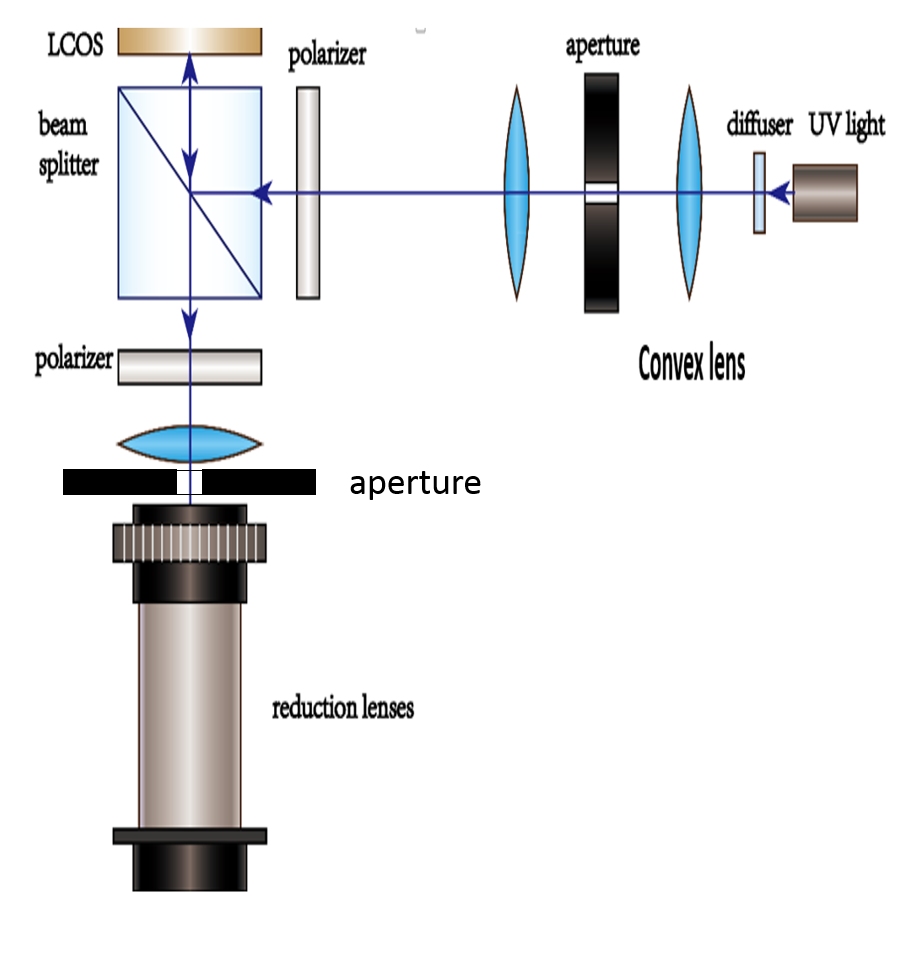
\includegraphics[width=0.8\textwidth]{lightpath.PNG}
  \caption{the illustration of the optical system}\label{figure_optical_path}
\end{figure}
\begin{itemize}
\item \textit{Convex lens}:
  \textbf{Converge} the uniform light emitted by \textit{UV LED source} into collimated light and function as the light 
  source of the LCOS. Two \textit{apertures} can be used to individually \textbf{adjust}\footnote{All the actions are set 
    to BOLD.} the diameter and brightness of the collimated beam.
\item \textit{Polarizing beam splitter}:
  The core part in the LCOS.
\item \textit{Reduction lens}:
  They were taken from the projectors and can reduce the image generated by the LCOS, which could be pretty big, before 
  projecting the image onto the printing plane. Every pixel in the reduced image should be equal to 15 micrometers in the 
  current optical path. The position and precision of the reduced image can be changed by simply \textbf{rotate} the lens.
\end{itemize}


\subsubsection{Motorized stage}
\textit{Motorized stage} consists of two parts.\underline{The first part} is \textit{stage plane} that can be moved in x,y 
direction. However, the stage position in x-y plane should be fixed under normal circumstances. \underline{The second part} 
is the piston that can be moved vertically in z-axis. \textbf{Remember} the positive direction for piston movement in z-axis 
is \underline{downwards}.
\begin{tabularx}{\textwidth}{ XXX} 
  \raisebox{-\height}{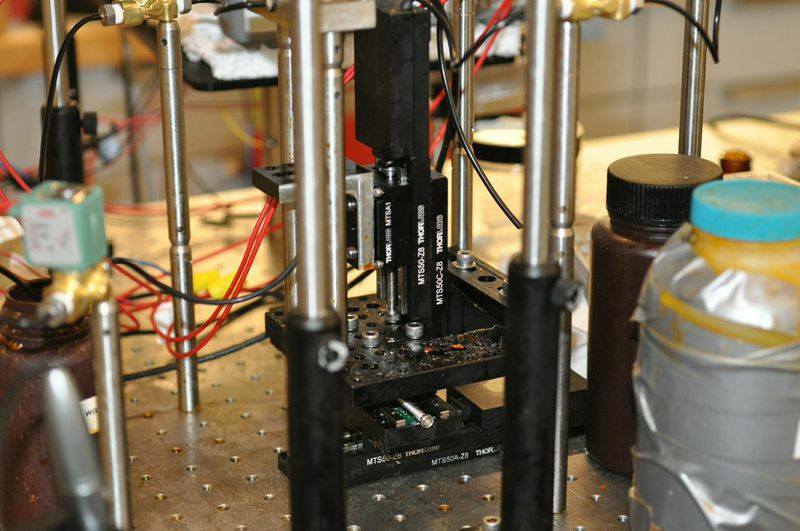
\includegraphics[width=0.3\textwidth]{motor.jpeg}}
  &\raisebox{-\height}{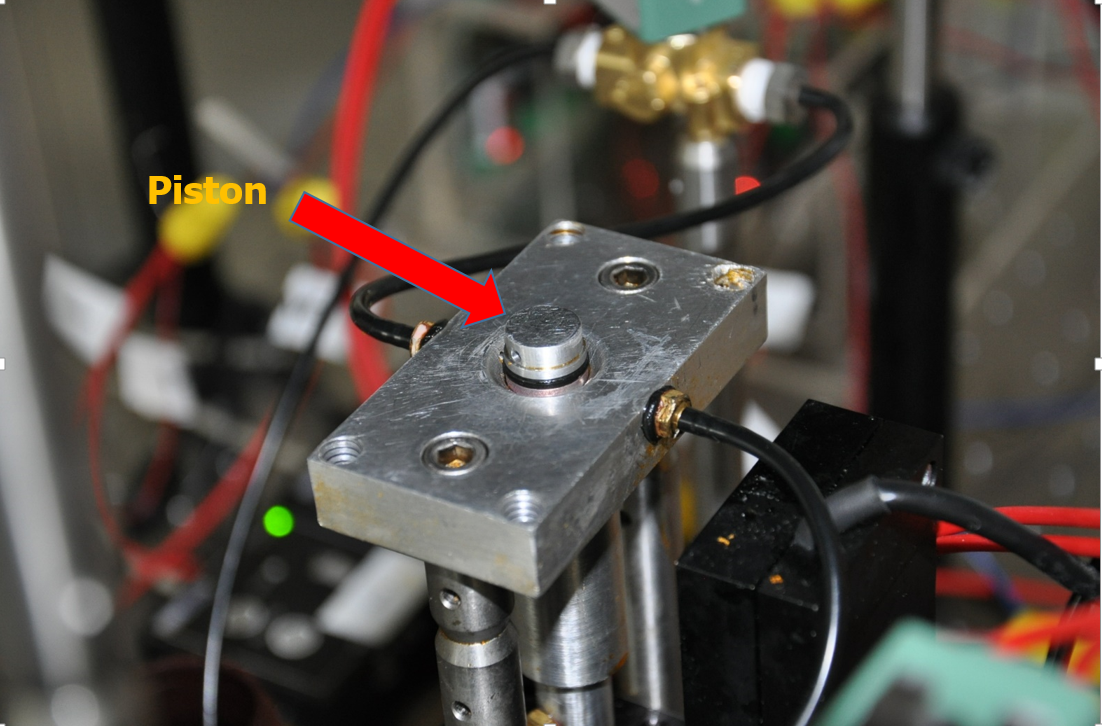
\includegraphics[width=0.3\textwidth]{step3_2.JPG}}
  &\raisebox{-\height}{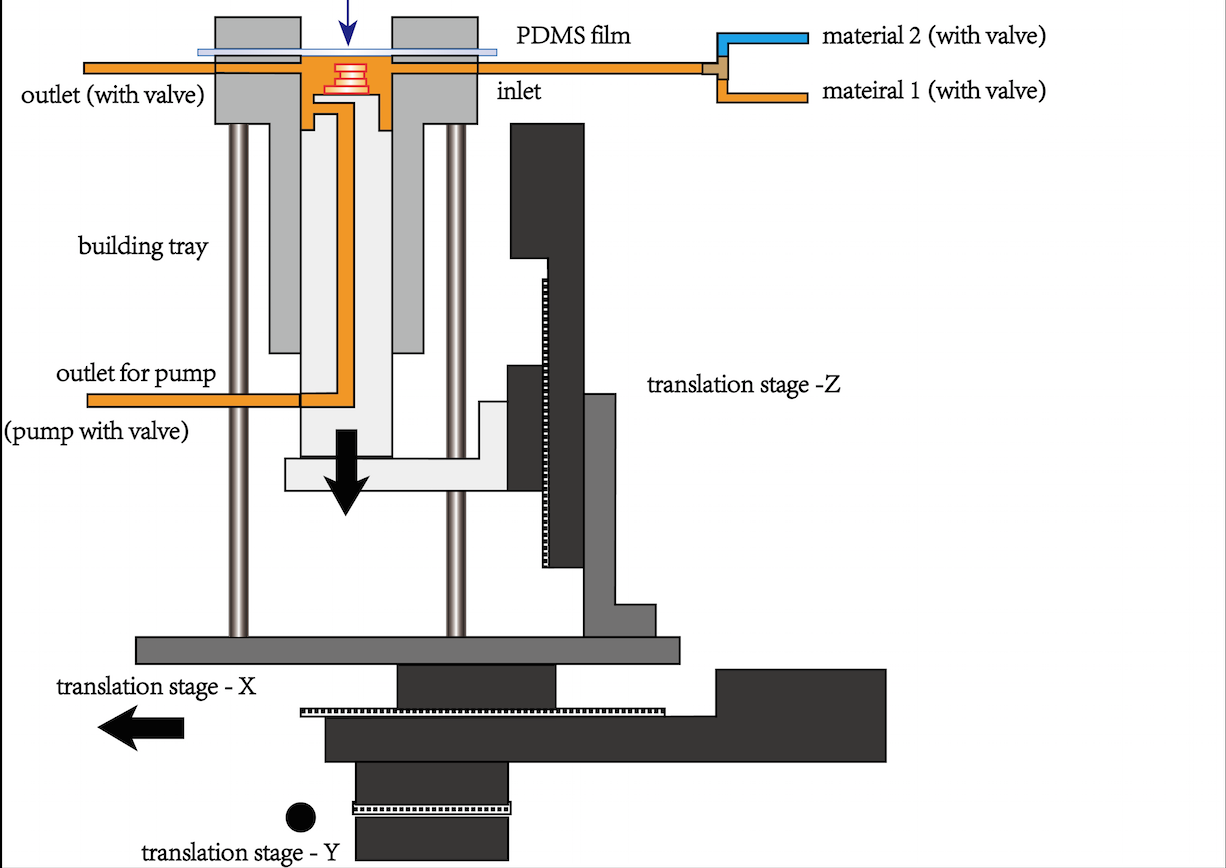
\includegraphics[width=0.3\textwidth]{stageil.png}}
  \\
\end{tabularx}

\subsubsection{Fluids system}
\textit{Fluids} system is consist of four \textit{valves} and several \textit{tubes}. The four valves and its connection 
via tubes on both left and right sides are listed as below in the table \ref{table_valve}:
\begin{table}
  \begin{center}
    \begin{tabular}{ | c | c | c |}
      \hline
      \textbf{name}&\textbf{left side connection}&\textbf{right side connection}\\ 
      \hline
      \textbf{valve for material 1 inlet}& chamber with prepolymer solution& material 1 inlet bottle\\     
      \hline
      \textbf{valve for material 2 inlet}& chamber with prepolymer solution& material 2 inlet bottle\\
      \hline
      \textbf{outlet valve}& waste bottle& chamber with prepolymer solution  \\
      \hline
      \textbf{pump valve}&pump which is connected to waste bottle& chamber with prepolymer solution\\ 
      \hline
    \end{tabular}
  \end{center}
  \caption{The left/right side connection of the valves} \label{table_valve}
\end{table}
\begin{tabularx}{\textwidth}{ XXX} 
  \raisebox{-\height}{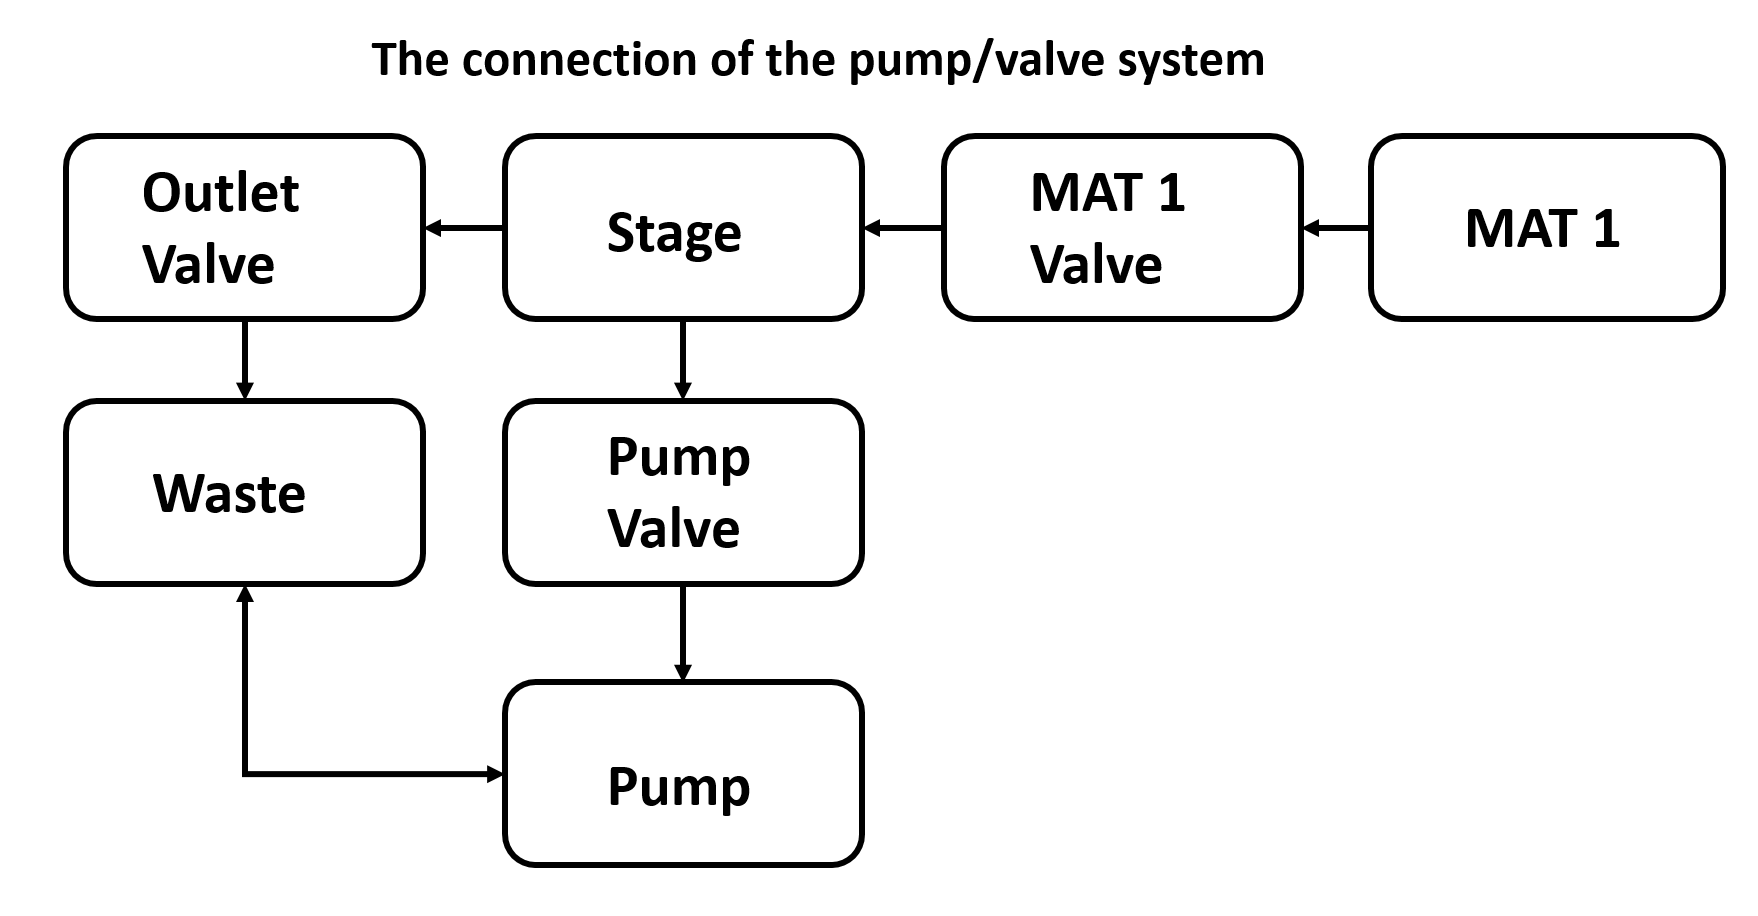
\includegraphics[width=0.3\textwidth]{bold.png}}
  &\raisebox{-\height}{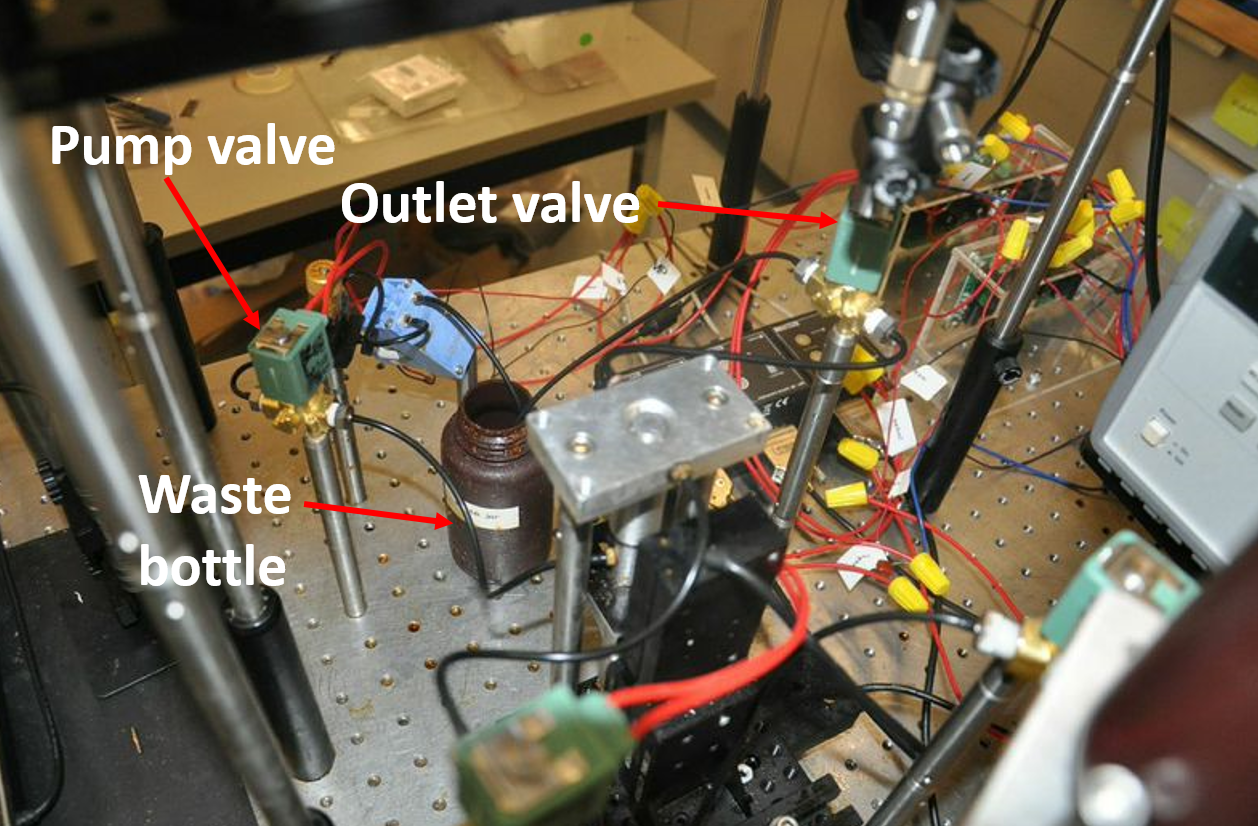
\includegraphics[width=0.3\textwidth]{valveil.PNG}}
  &\raisebox{-\height}{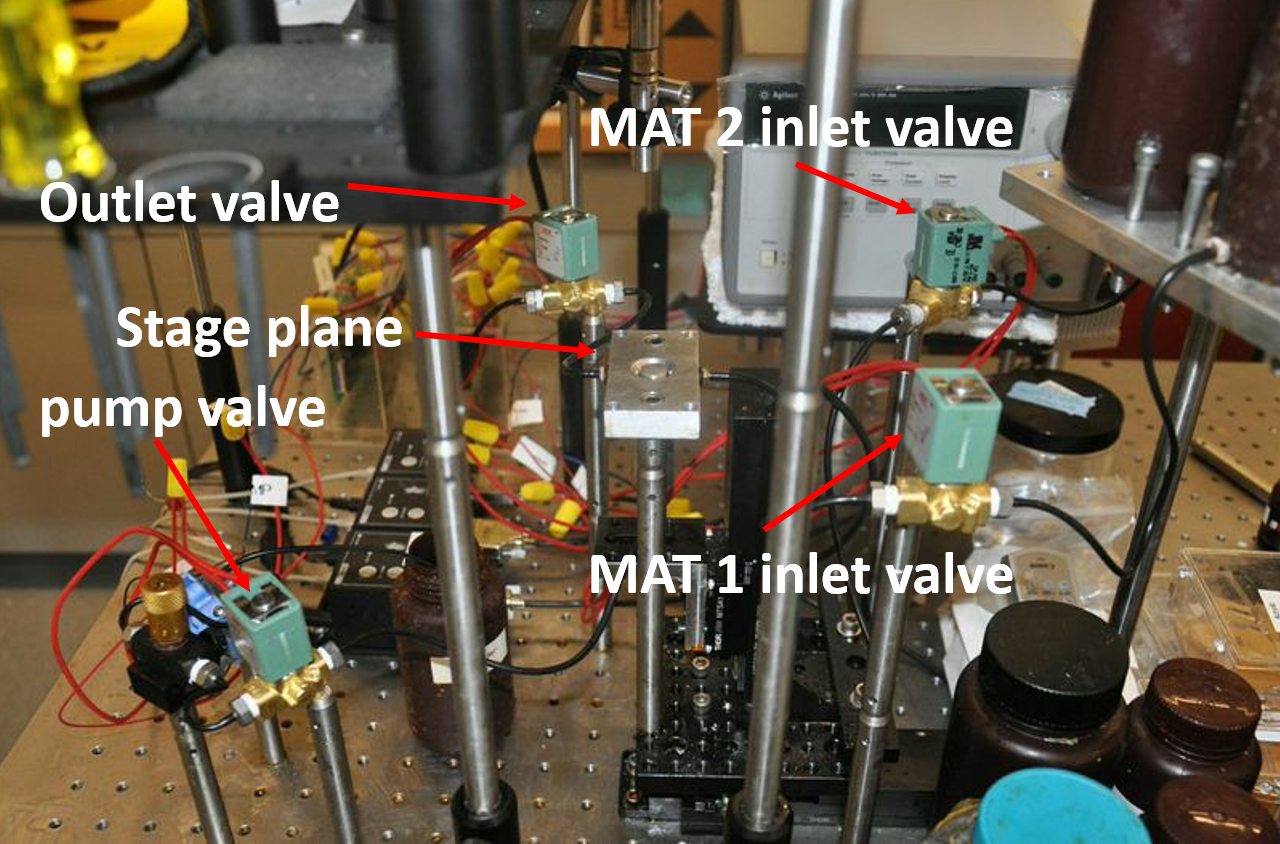
\includegraphics[width=0.3\textwidth]{il.PNG}}
  \\
\end{tabularx}



\subsubsection{Powersupply}
\textit{Powersupply} (Agilent E3633A) powers the \textit{electrical device(UV light, valve)}
in the system. \textbf{Check} operation manual for details\footnote{http://www.trs-rentelco.com/Specs-Manuals/AT\_E3633A\_Manual.pdf}.\\
\begin{tabularx}{\textwidth}{ XXX} 
  \raisebox{-\height}{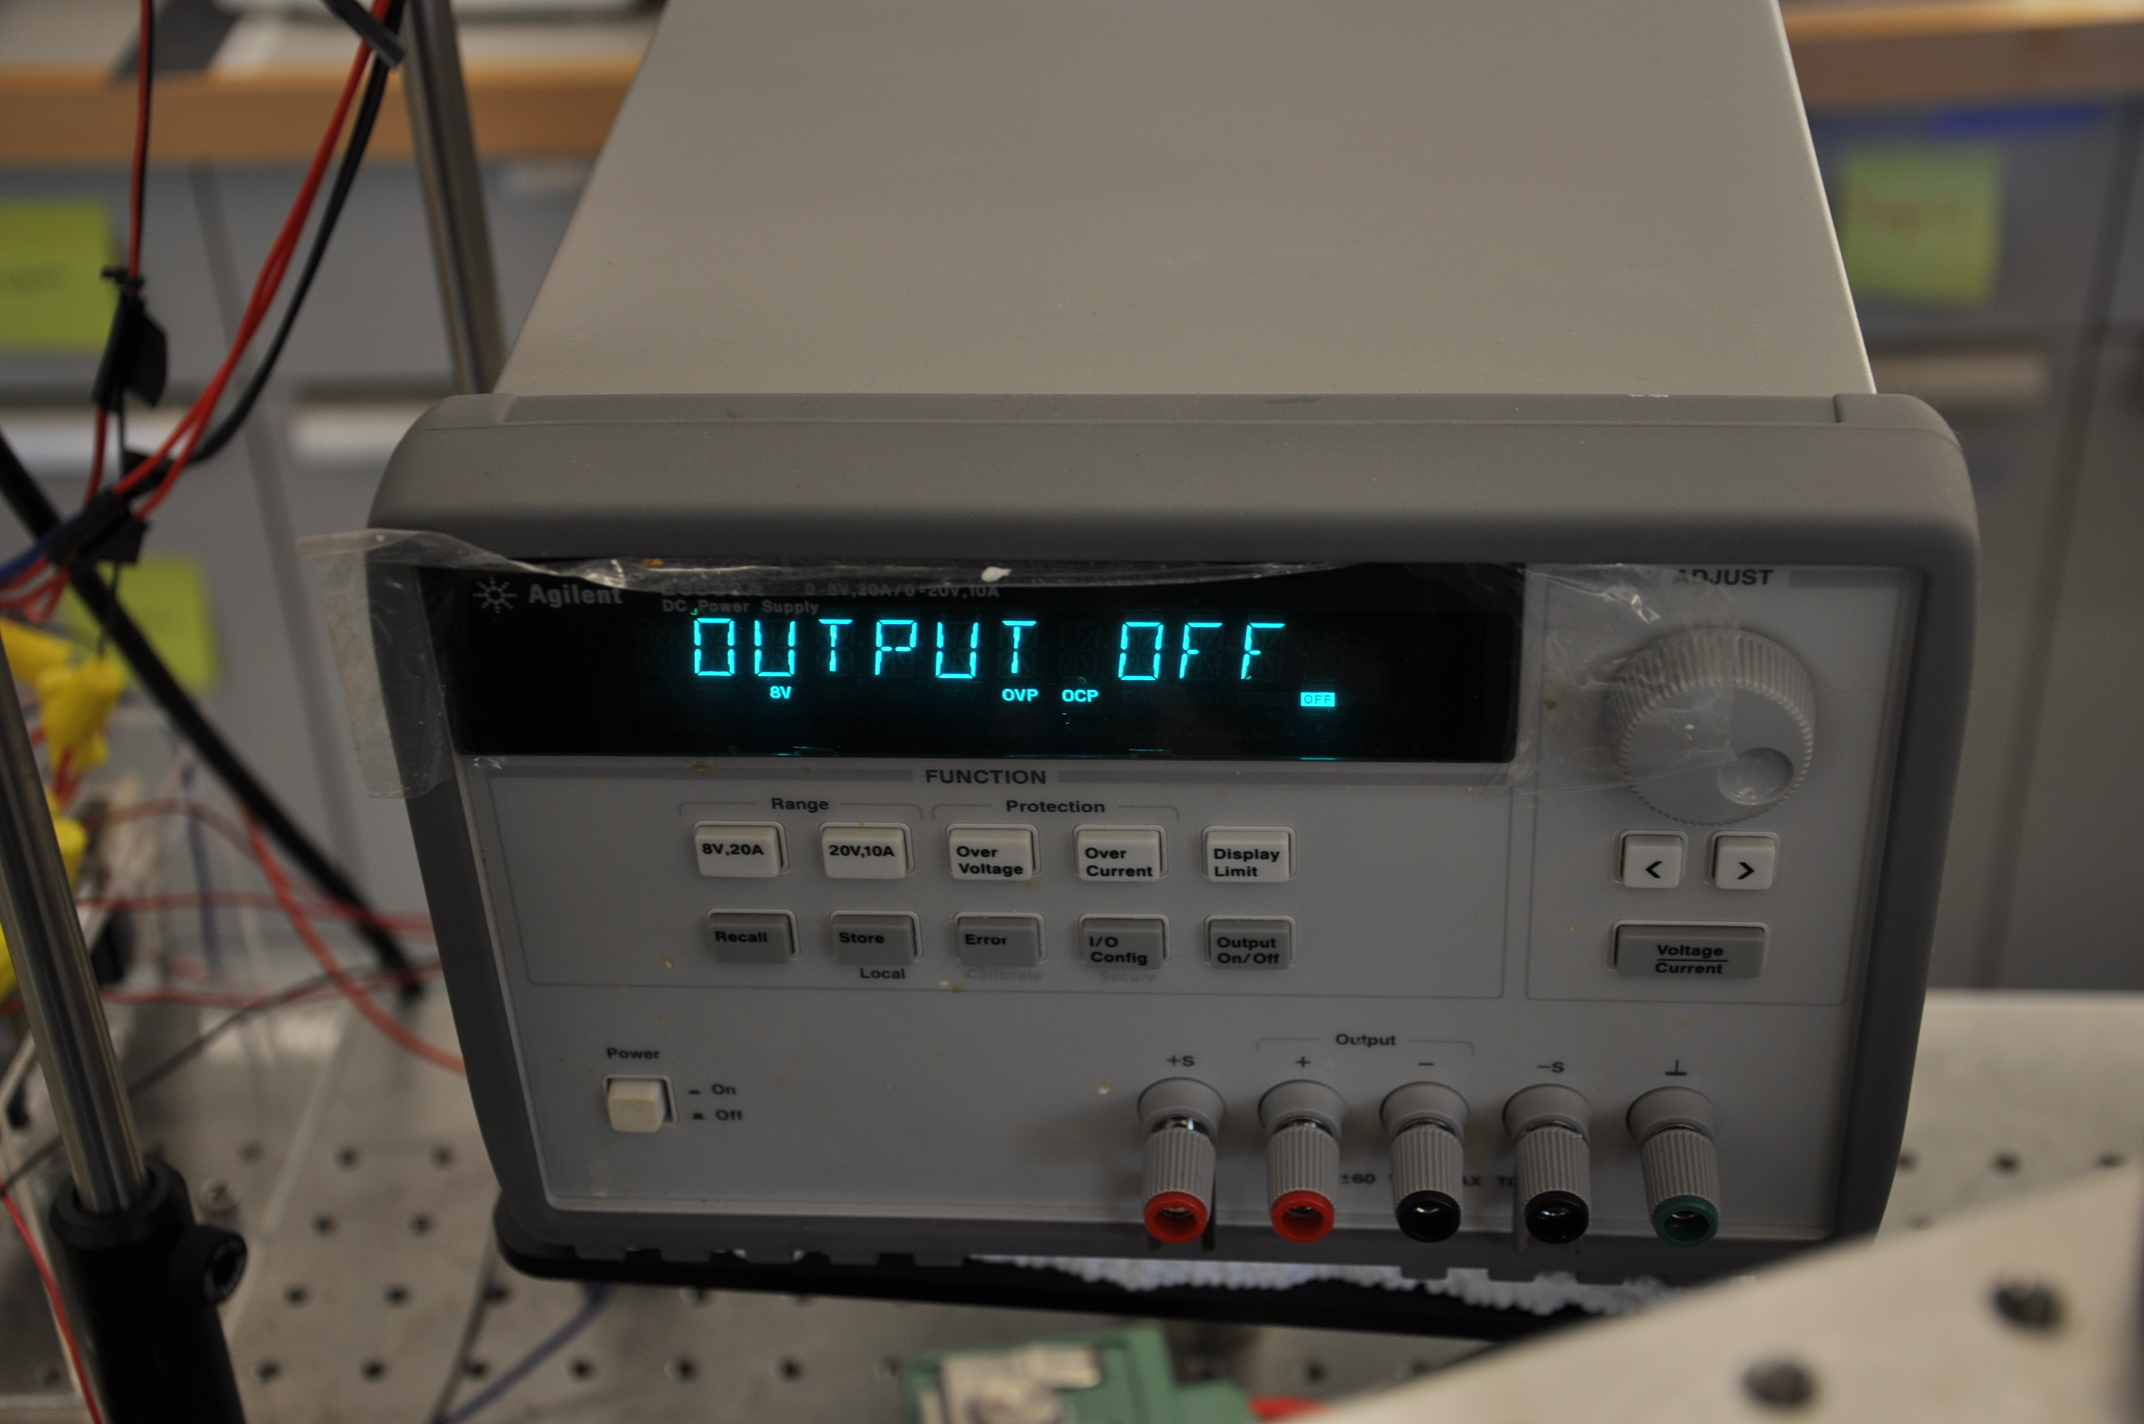
\includegraphics[width=0.3\textwidth]{outputoff.JPG}}
  &\raisebox{-\height}{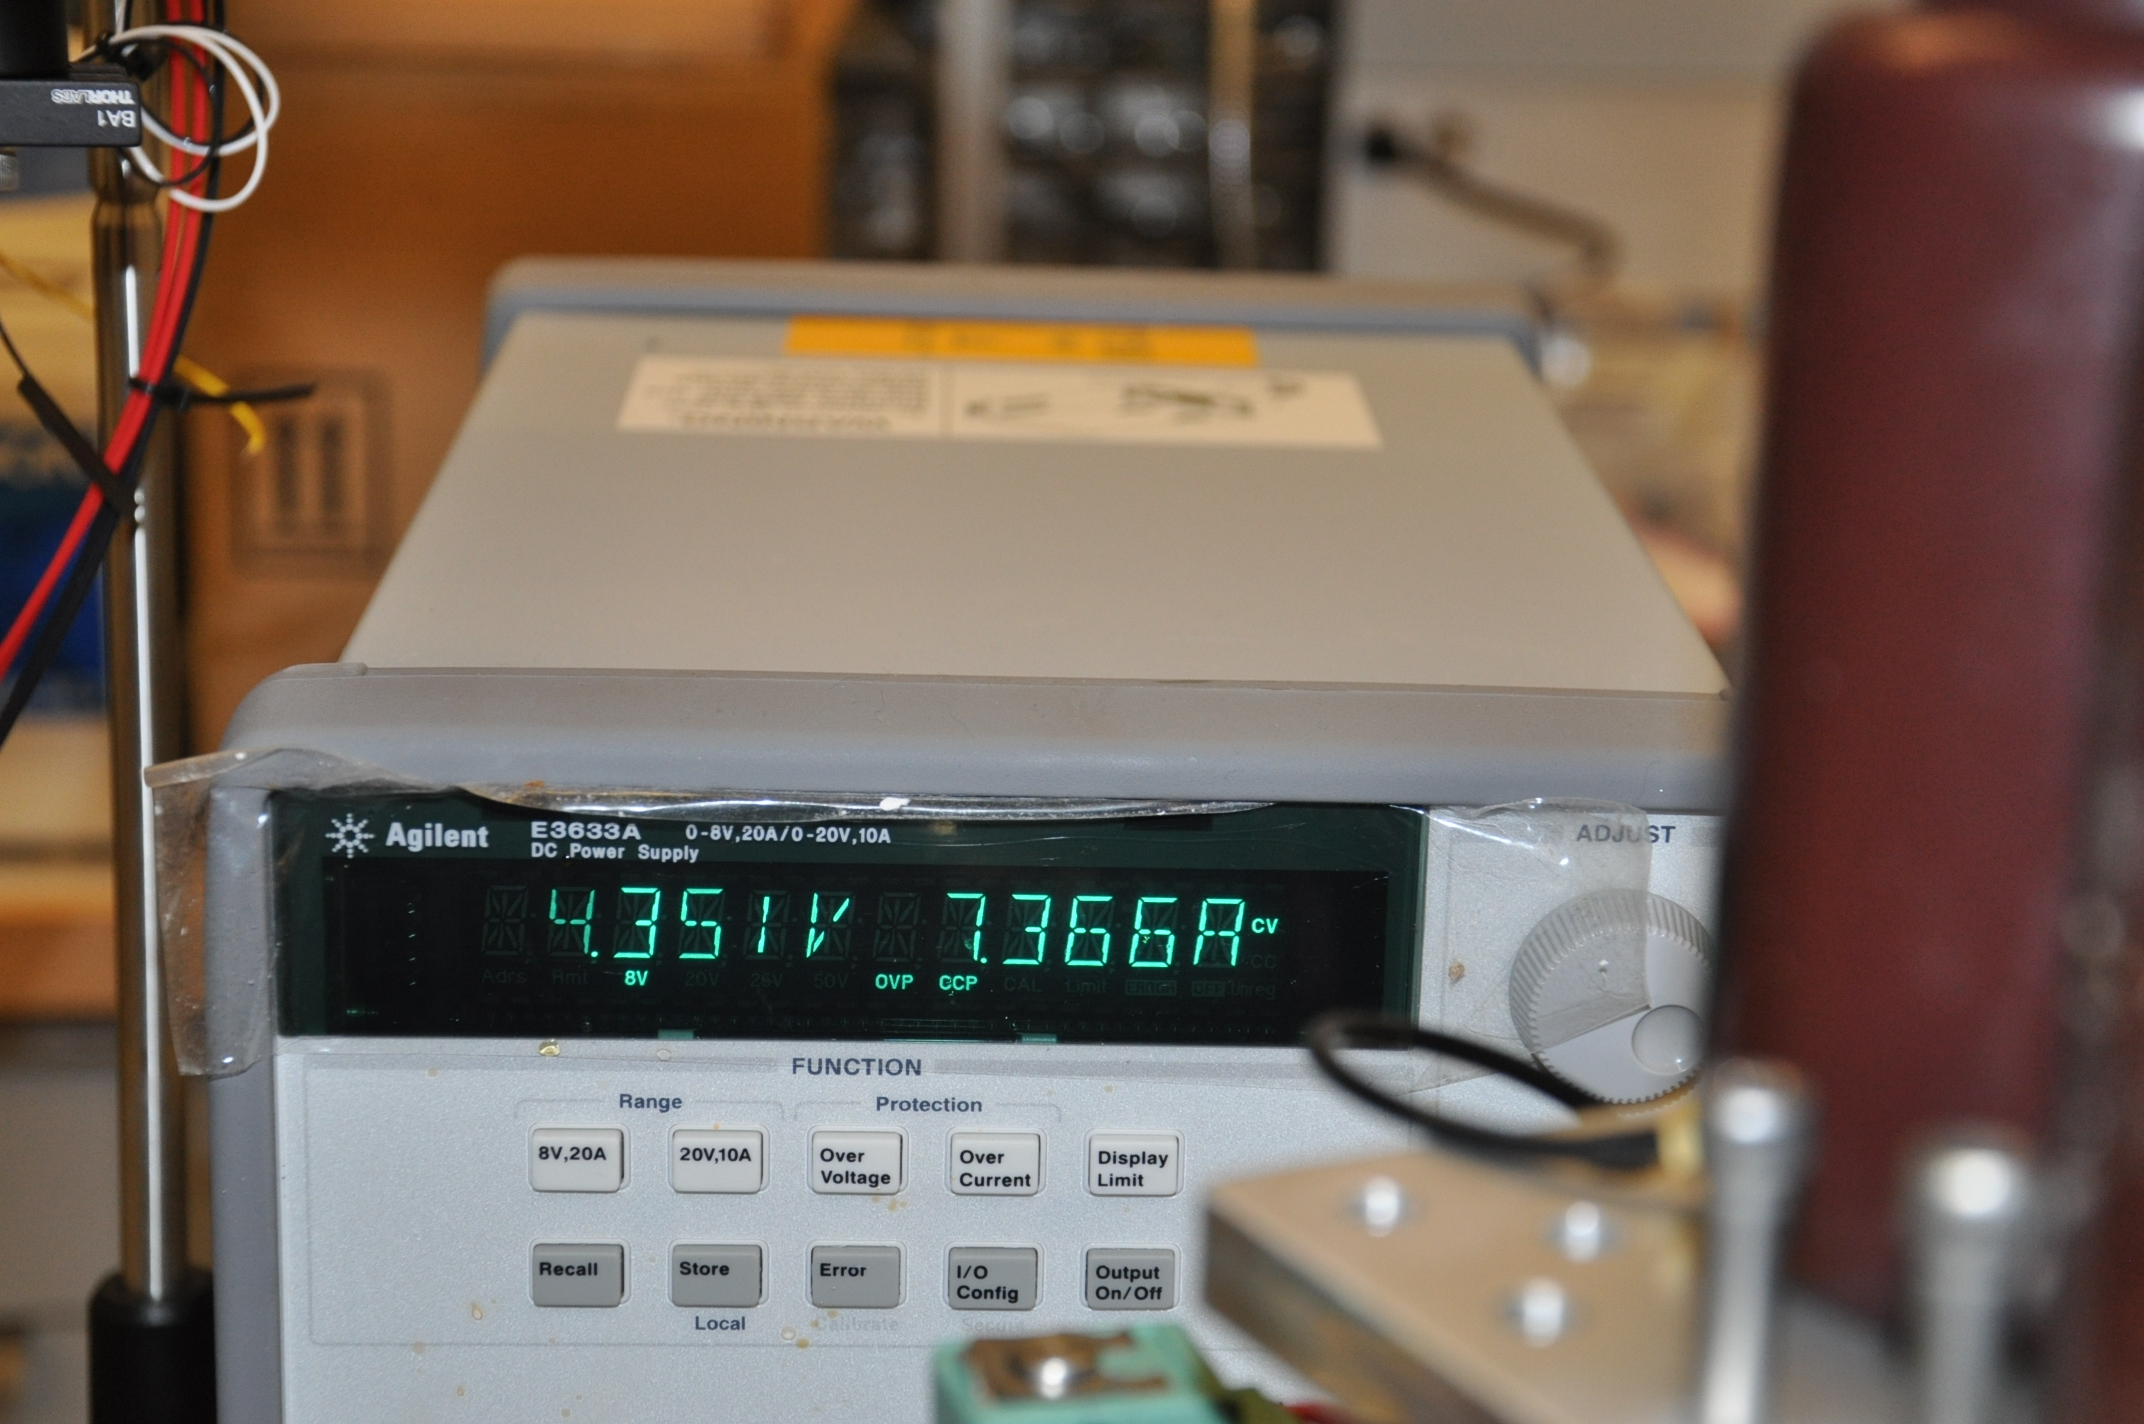
\includegraphics[width=0.3\textwidth]{step5_2.JPG}}
  &\raisebox{-\height}{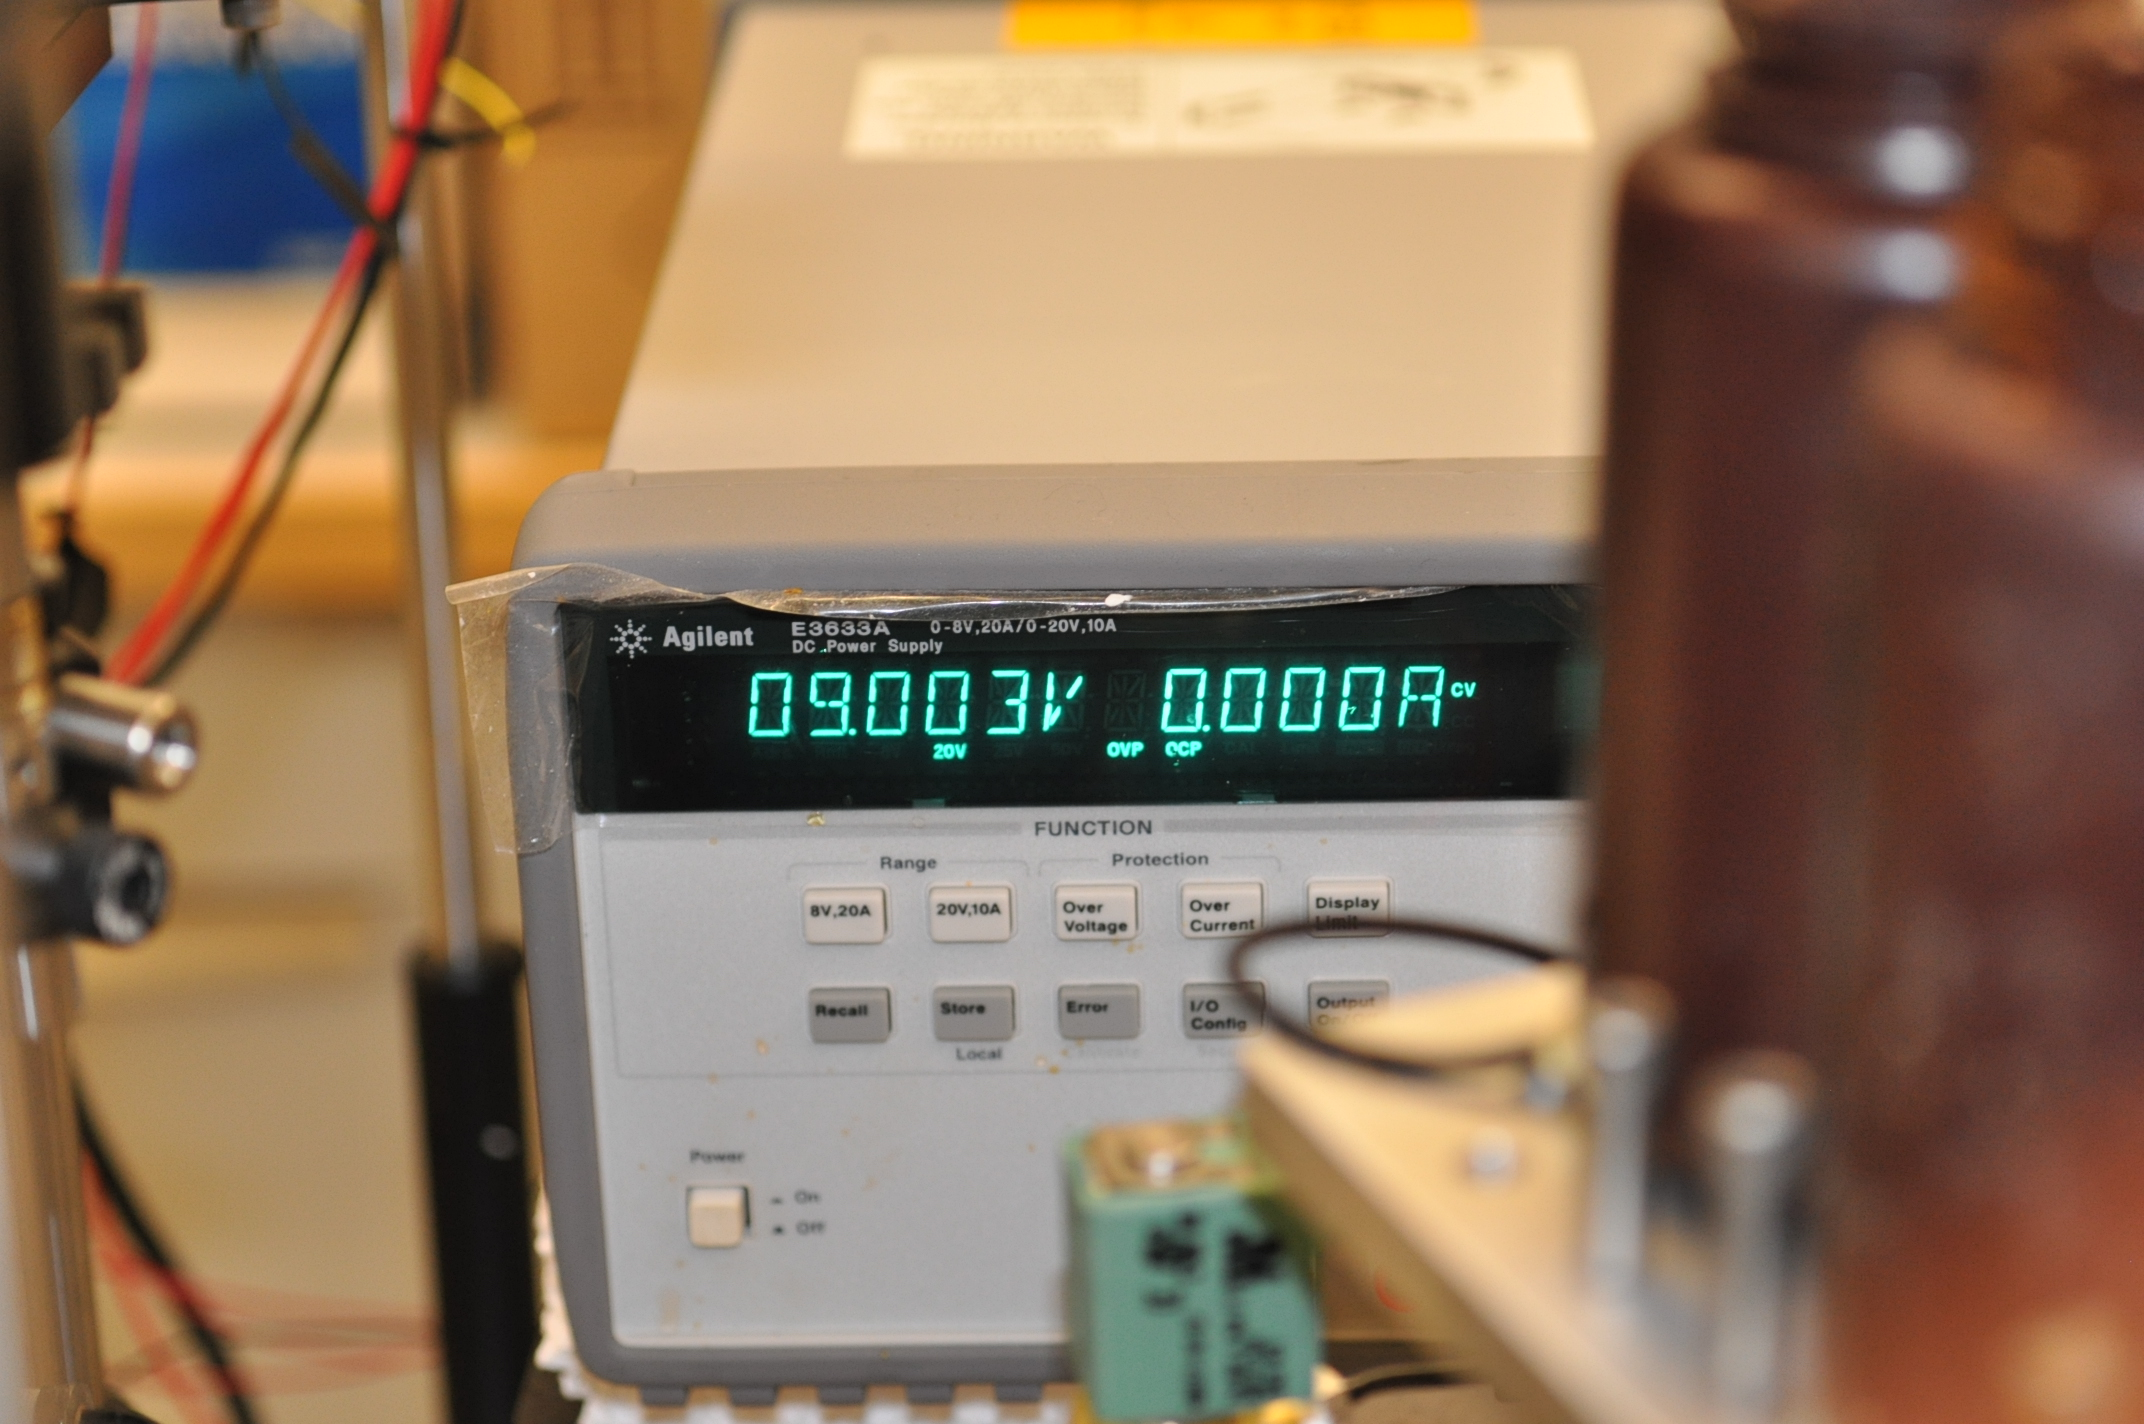
\includegraphics[width=0.3\textwidth]{step8_display.JPG}}
  \\
\end{tabularx}



\subsubsection{Printing chamber}
\textit{Printing Chamber} is enclosed by a customer-made cover , which is composed of two laminated parts fixed together 
by the screws. The top part is an octagonal acrylic board with a circular opening in the middle and several openings designed 
for screw-bonding at the periphery. The lower part is a piece of PDMS film used for creating an oxygen-free environment within 
the \textit{chamber}. The cover is fixed onto the stage through screws in the corner.The \textit{piston} can move vertically 
within the chamber to perform the priting.
\begin{tabularx}{\textwidth}{ XXX} 
  \raisebox{-\height}{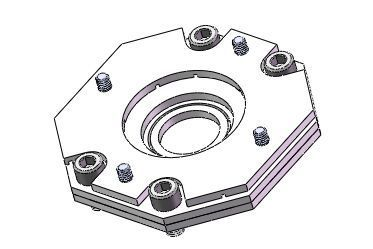
\includegraphics[width=0.3\textwidth]{chamber.jpeg}}
  &\raisebox{-\height}{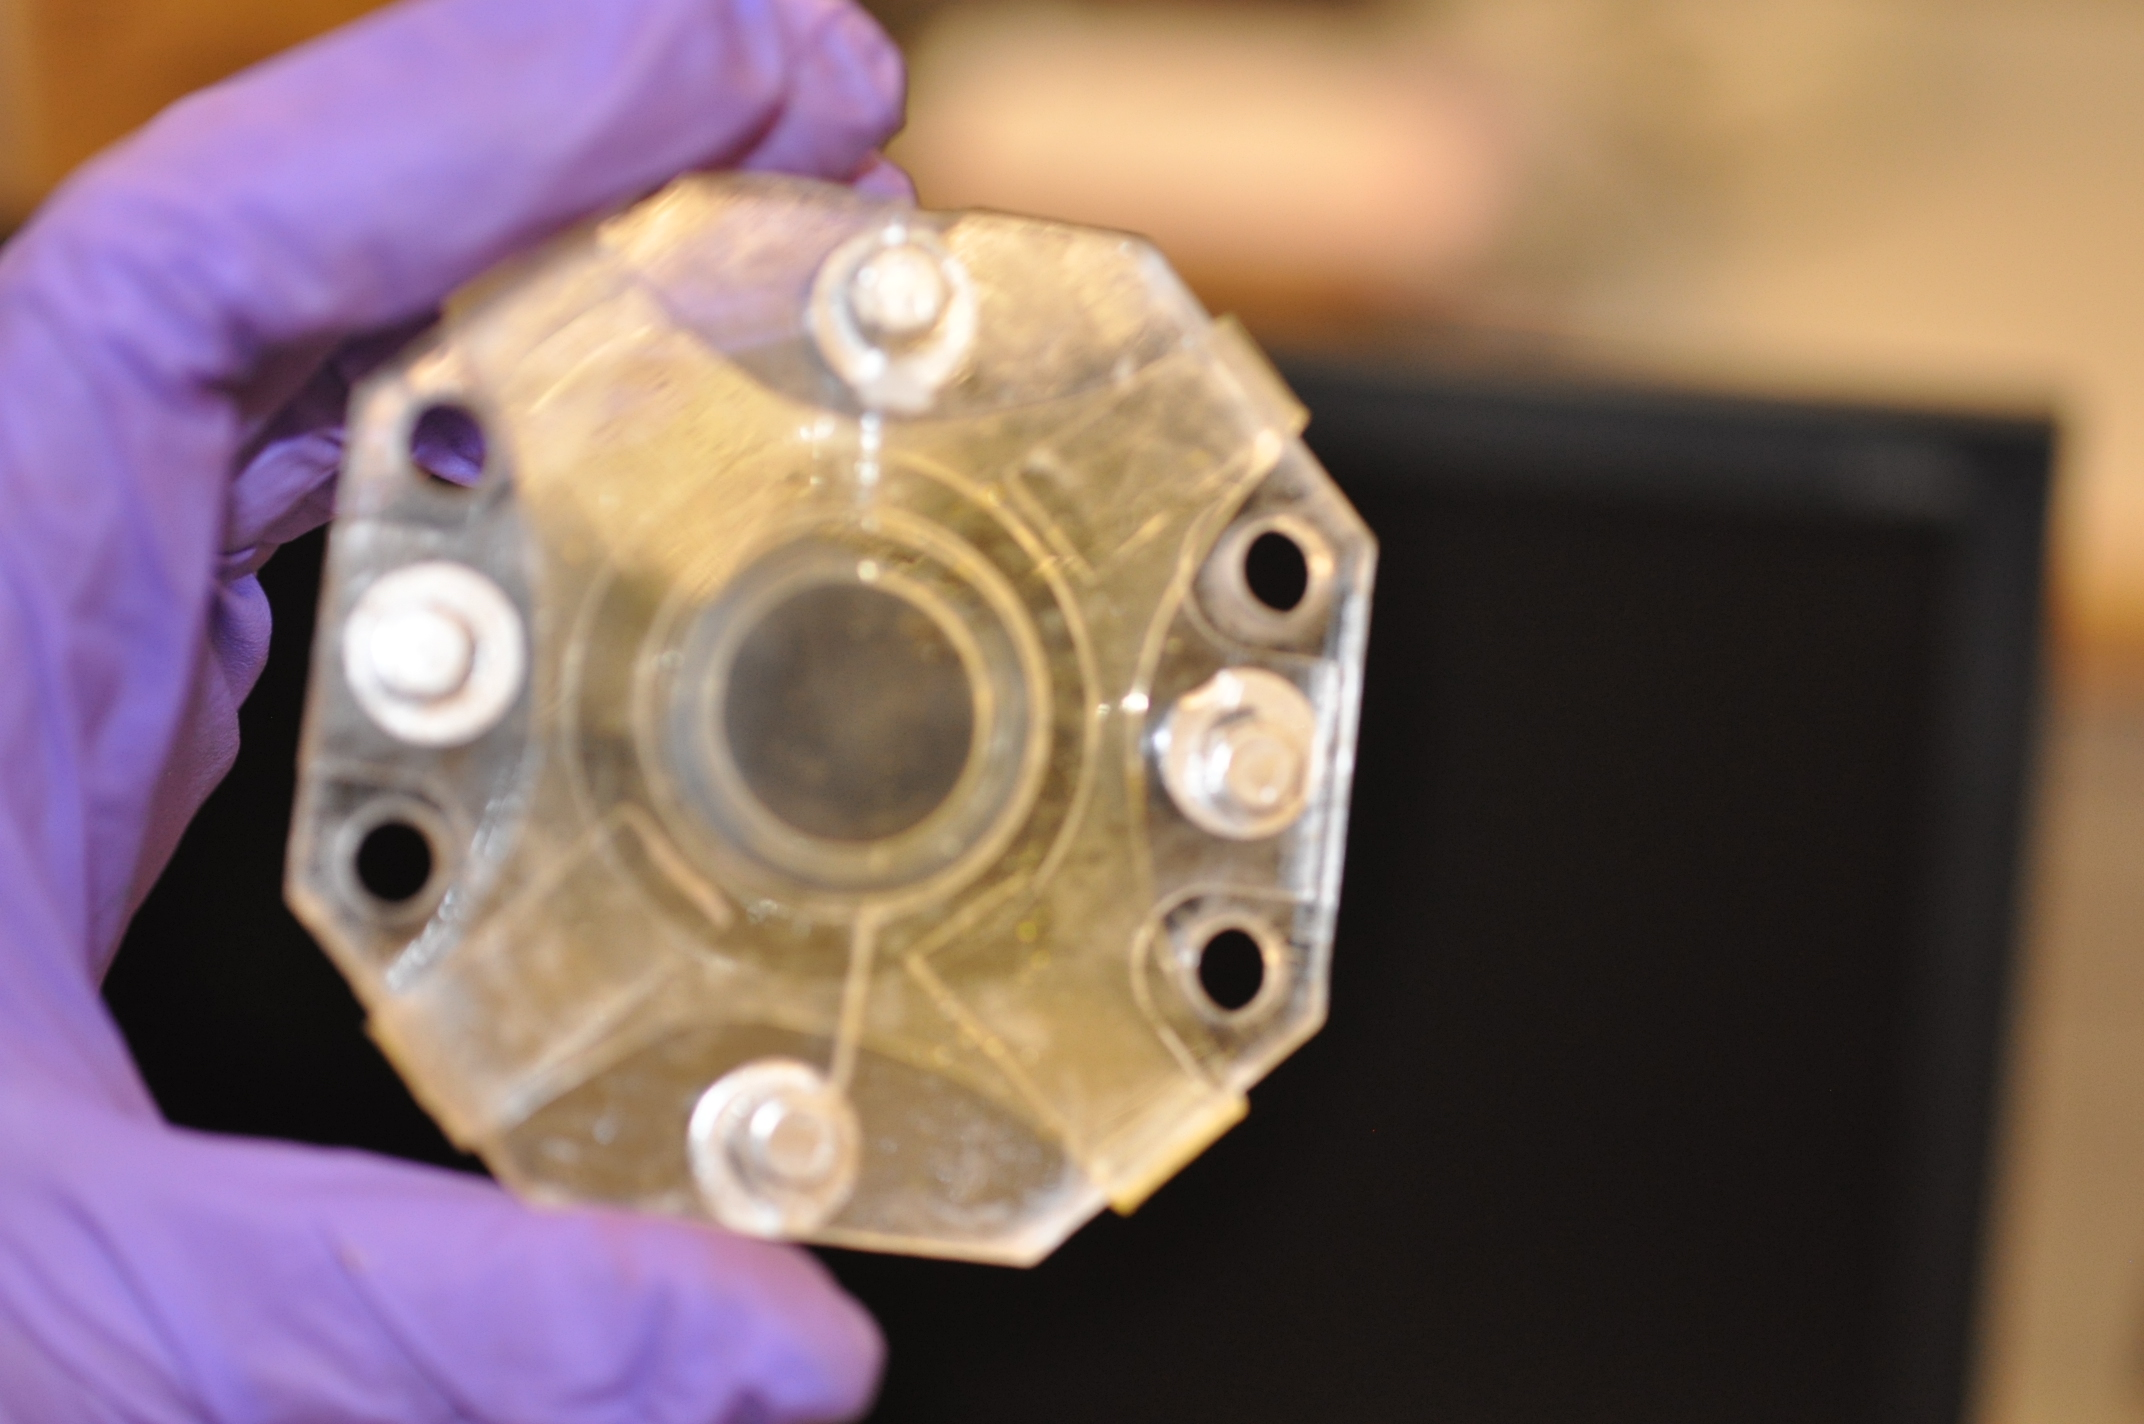
\includegraphics[width=0.3\textwidth]{chamber.JPG}}
  &\raisebox{-\height}{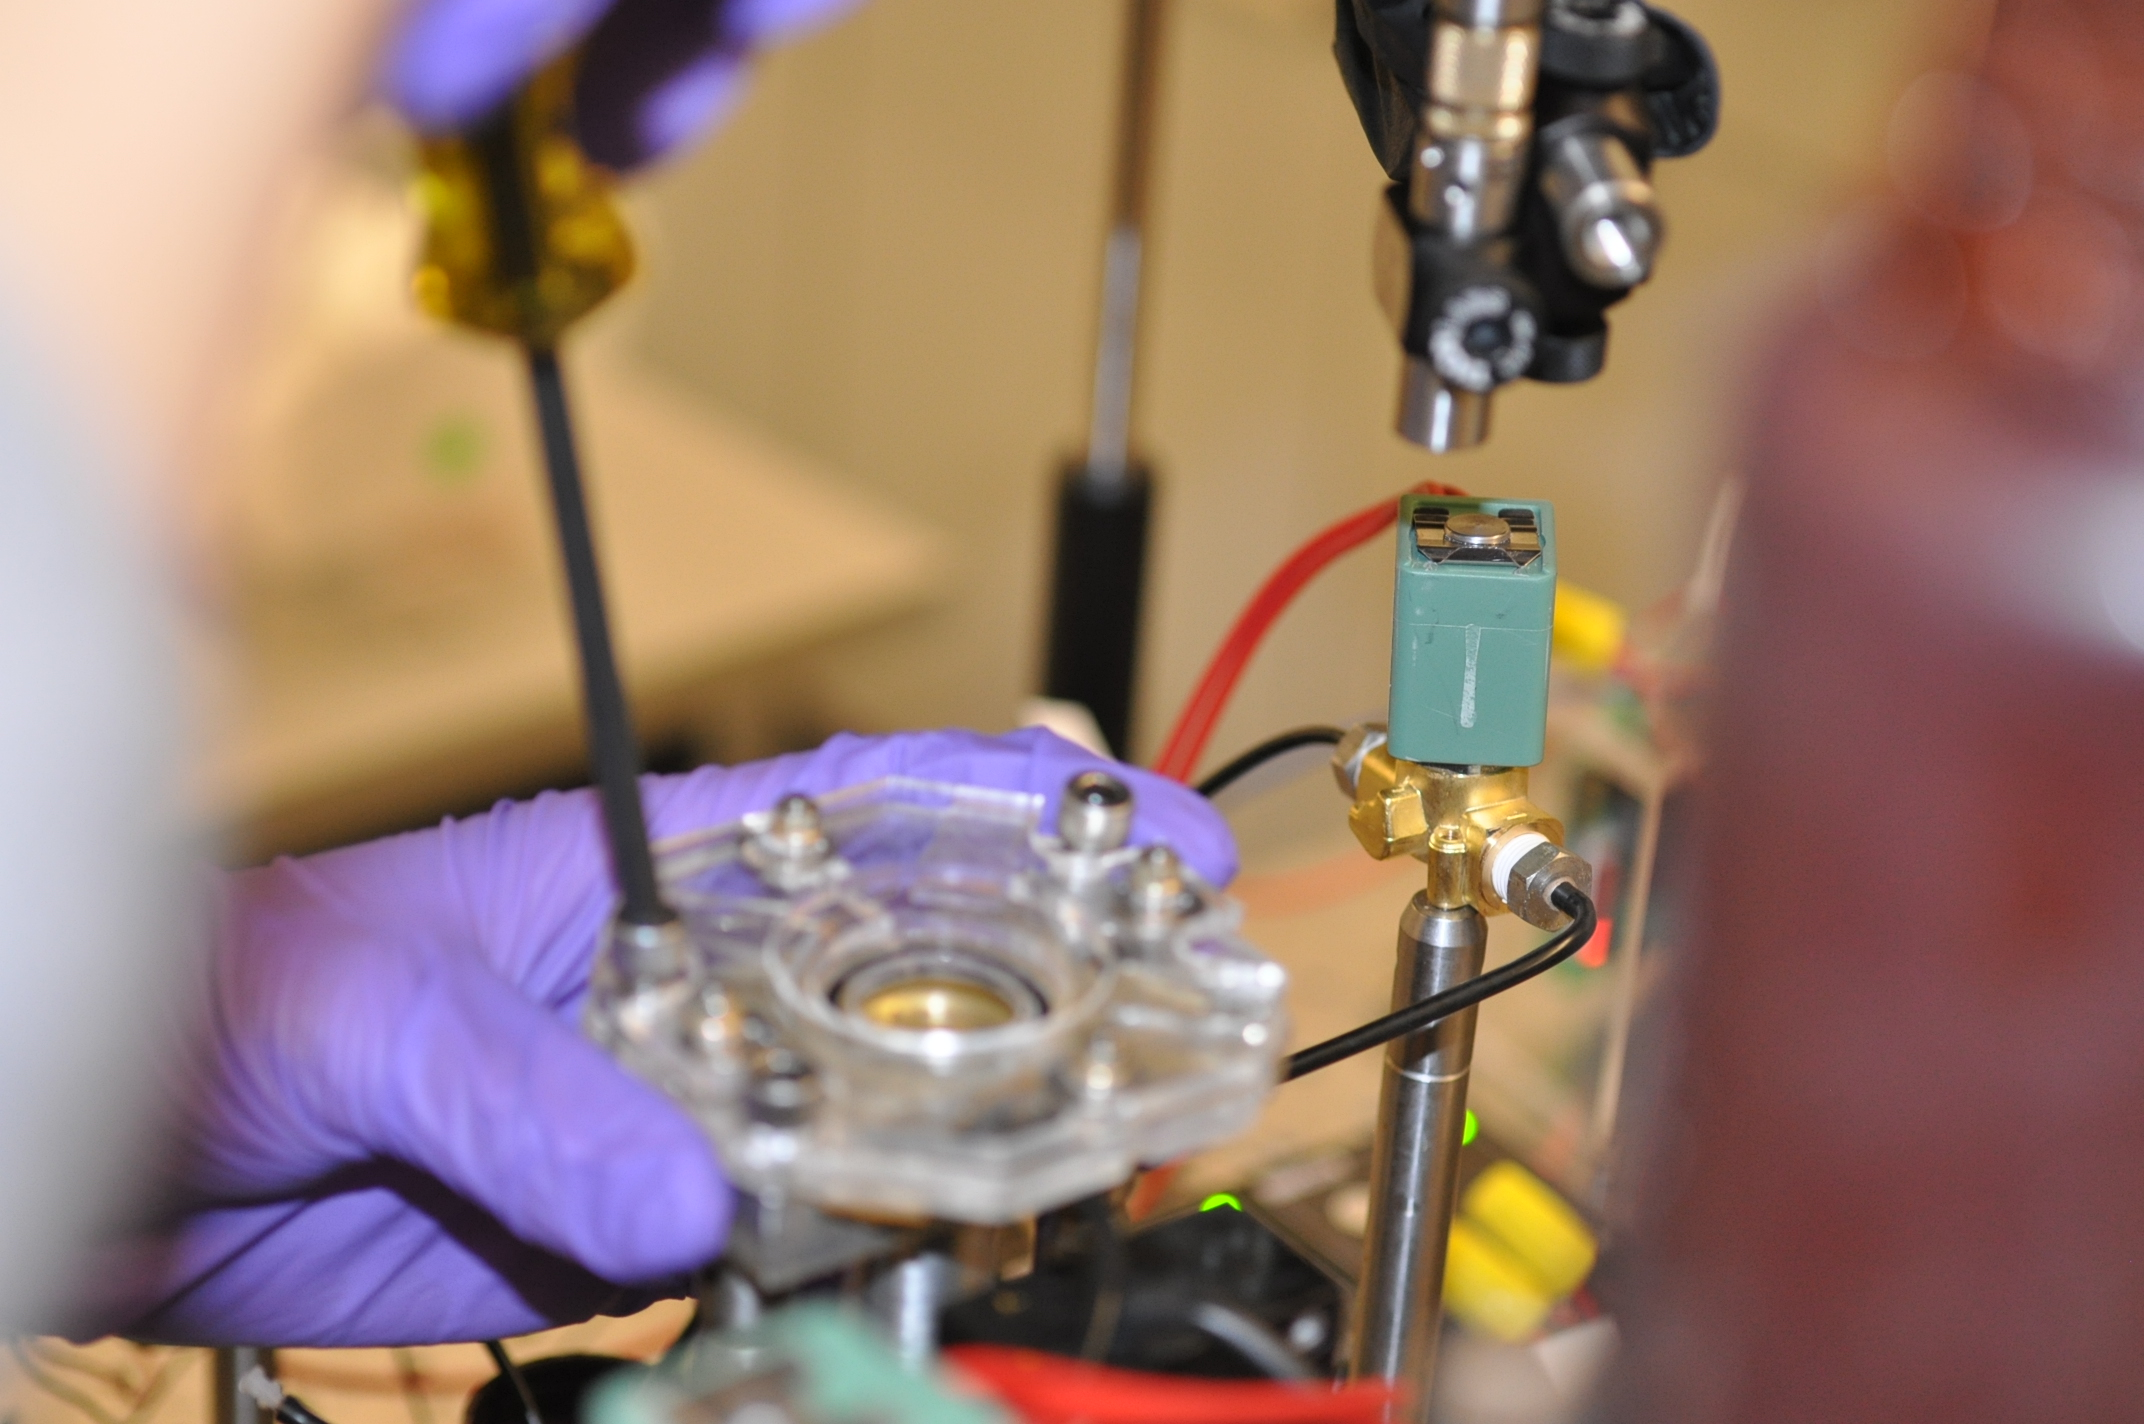
\includegraphics[width=0.3\textwidth]{Step9_bonding.JPG}}
  \\
\end{tabularx}

\subsubsection{Electronic Microscope}
\textit{Supereye} is a hand-held microscopic device. \textbf{Click} open the \textit{Supereye} icon at the desktop, and the 
microscopic image of the printed sample can be easily observed from the computer screen \textit{in details}. It could also be 
used to observe the precision of the projected image at \ref{step 6} step 6.The definition of the image on display could  be 
changed by \textbf{rotating} the knob at the top of the \textit{supereye}. The scale of the microstruture could also be 
\textbf{measured} on the software interface.
\begin{tabularx}{\textwidth}{ XXX} 
  \raisebox{-\height}{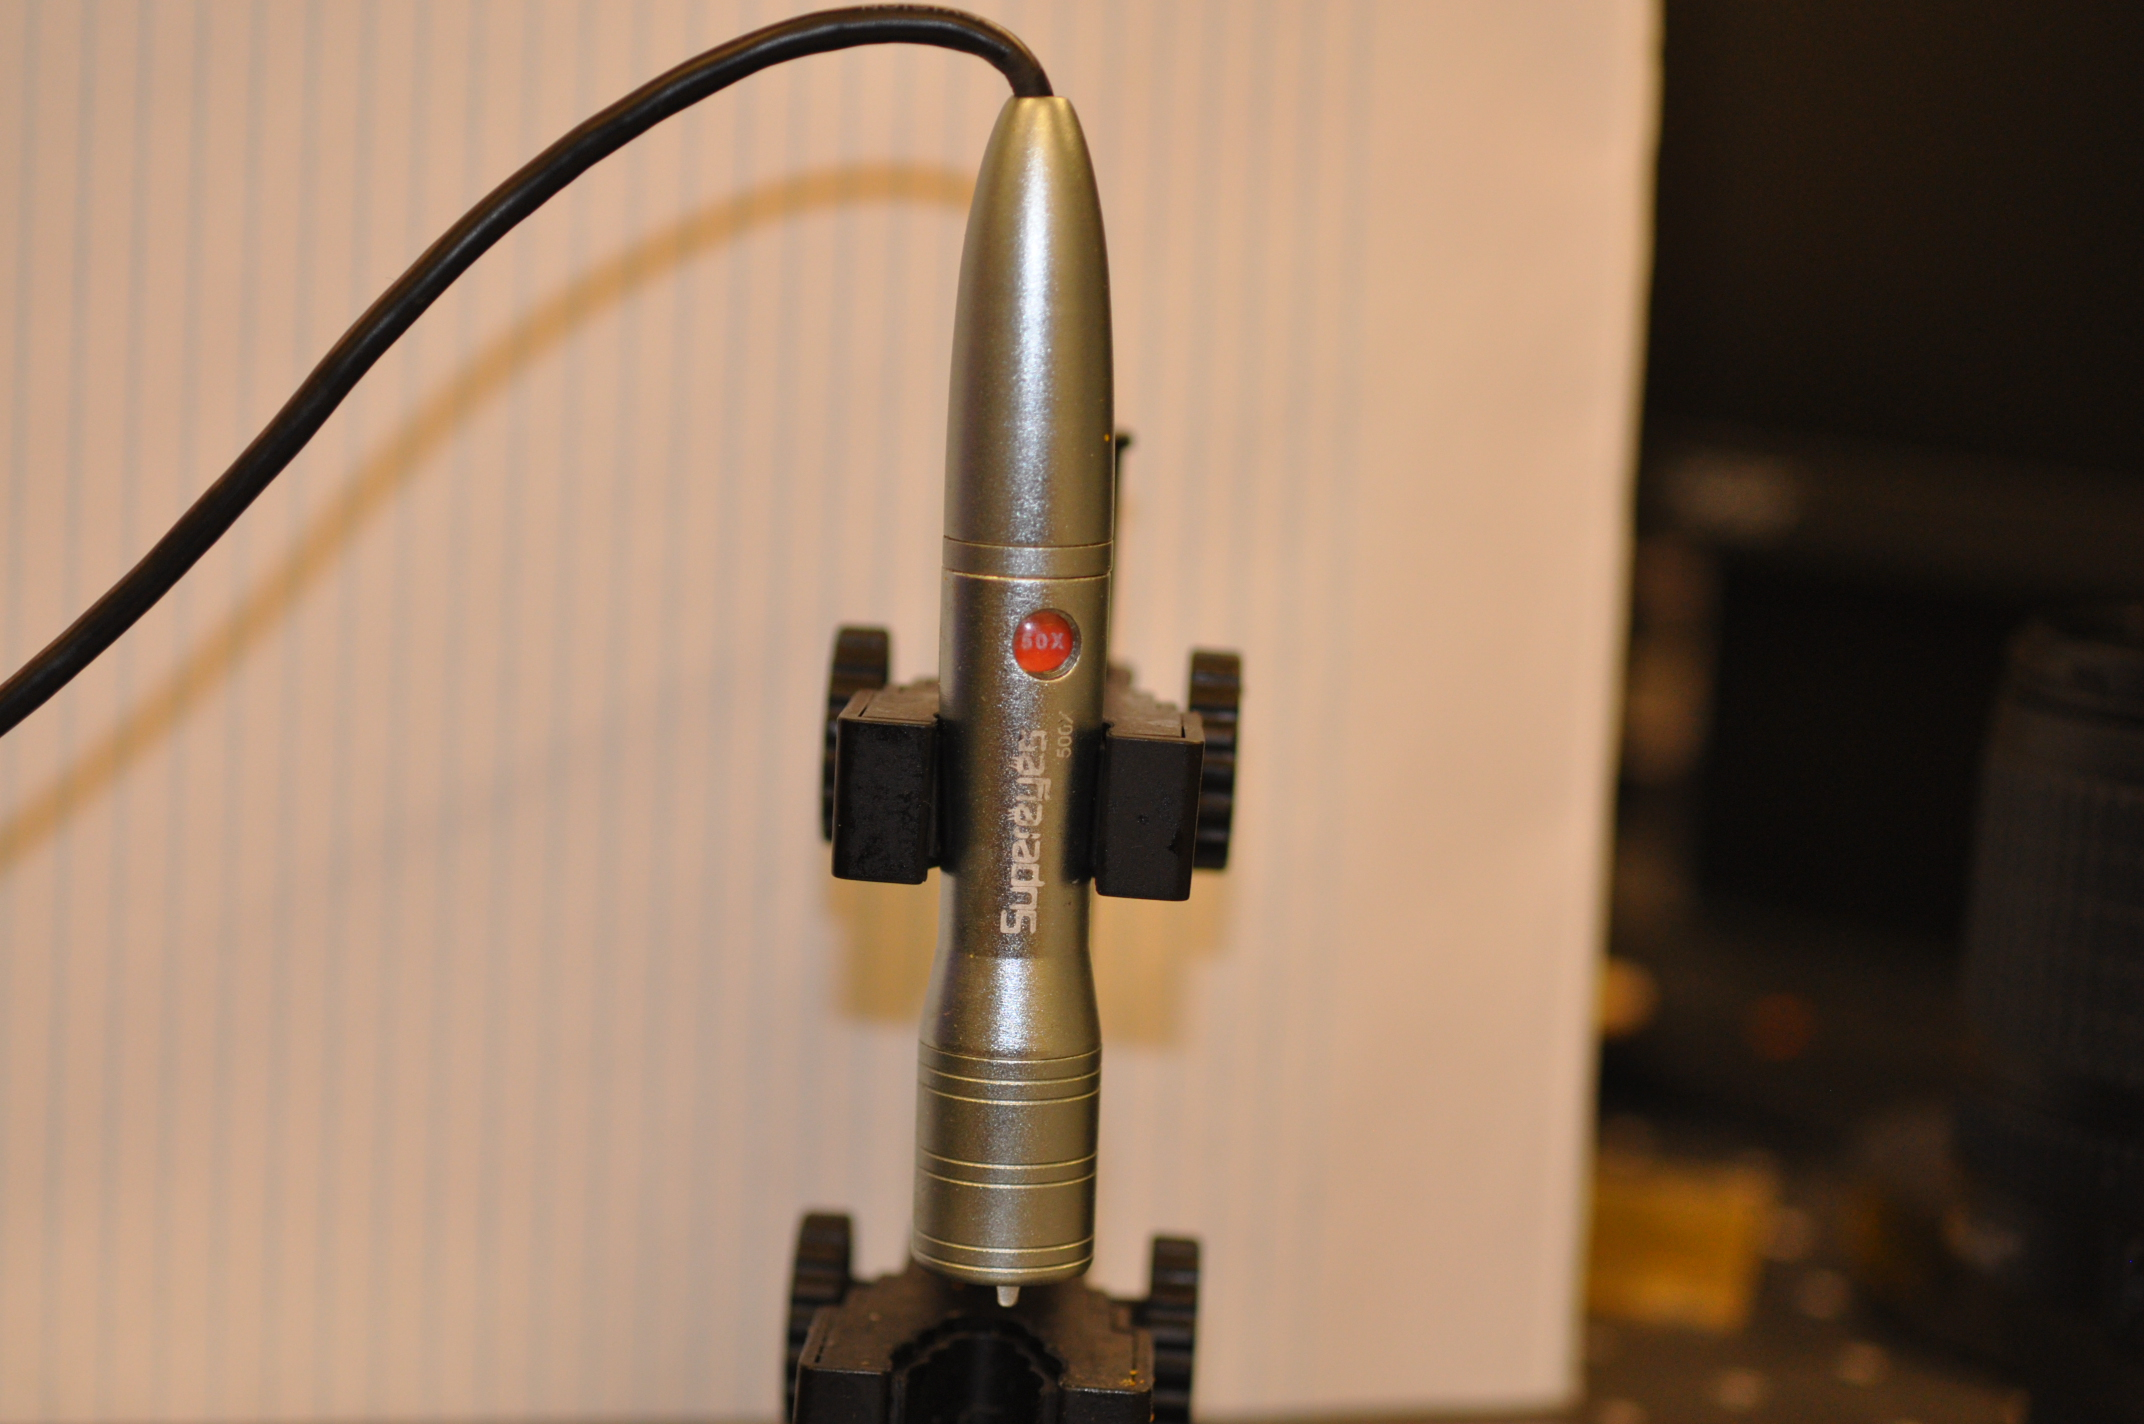
\includegraphics[width=0.3\textwidth]{supereye.JPG}}
  &\raisebox{-\height}{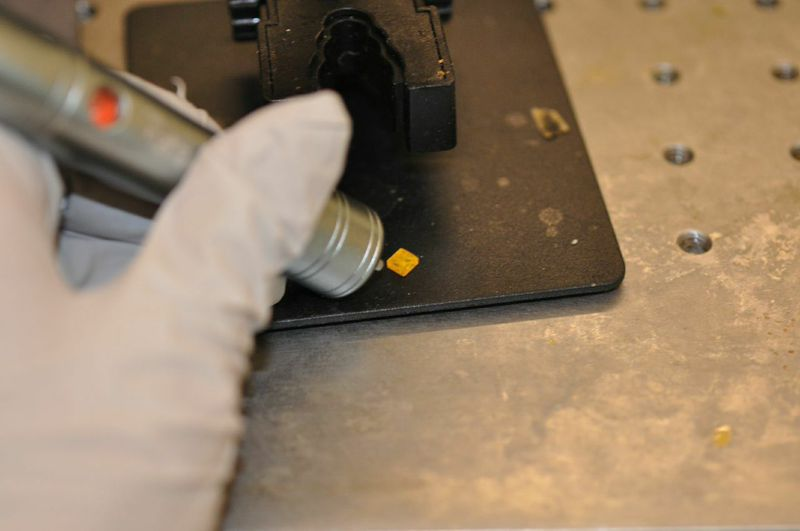
\includegraphics[width=0.3\textwidth]{supereyeob.jpeg}}
  &\raisebox{-\height}{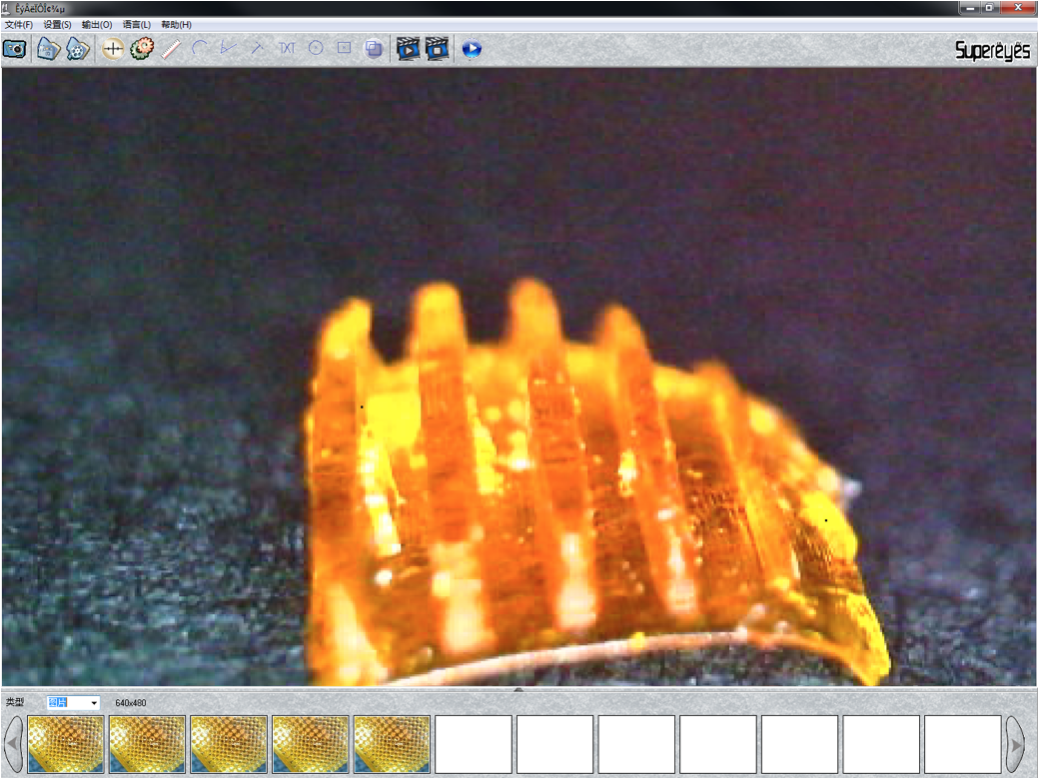
\includegraphics[width=0.3\textwidth]{sample.jpeg}}
  \\
\end{tabularx}

\pagebreak

\subsection{Software}
\subsubsection{User interface in Labview}
There are \textbf{three parts} that need to be highlighted in the labview interface: \textit{motorized stage control part, 
valve/UV LED control part} and \textit{printing control part}
\begin{figure}
  \centering
  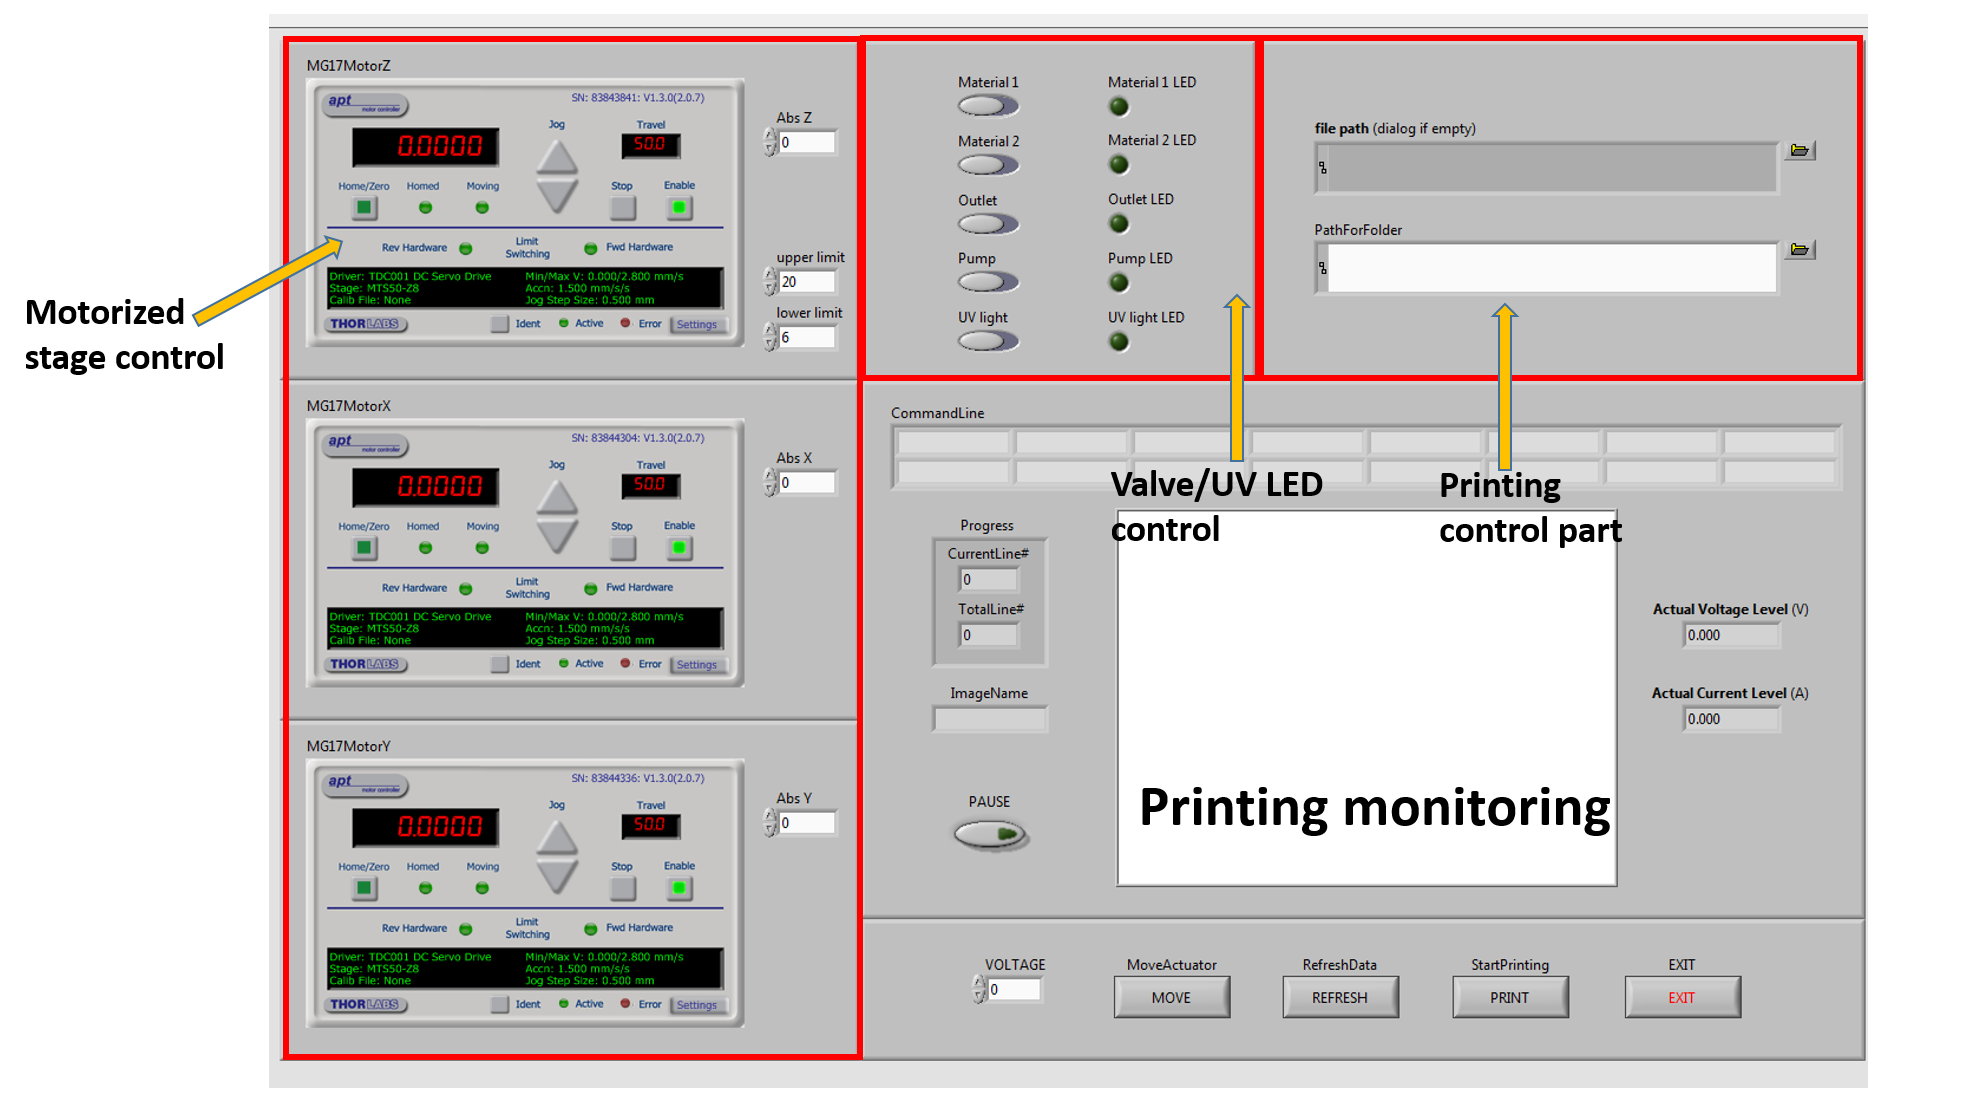
\includegraphics[width=400pt]{labview1.PNG}
  \caption{The illustration of the user interface in Labview}
\end{figure}

The three stage control parts from top to bottom individually adjust the stage movement in z,x,y axis. \textbf{Home} Z axis 
every time \textit{Labview} is started while \underline{never home x,y axis unless there is an assembly need}. \textbf{Type 
in} the values to change the stage position. The default parameter is recommended for the z-axis movement while you can 
\textbf{change} it according to your need by \textbf{clicking} \textit{settings} at the lower-right corner.
\begin{tabularx}{\textwidth}{XX}
  \raisebox{-\height}{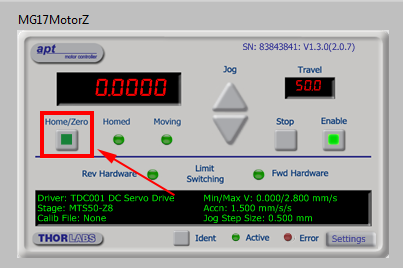
\includegraphics[width=0.4\textwidth]{step3_1.png}}
  &\raisebox{-\height}{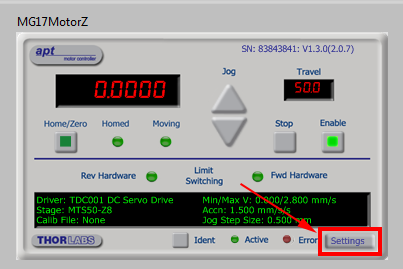
\includegraphics[width=0.4\textwidth]{step4_1.png}}
  \\
\end{tabularx}

In the valve/UV LED interface, a \textbf{click} is all you need to open the valve and the UV LED. \underline{Remember not to 
  simultaneously open the \textit{valve} and the \textit{UV LED} because of the following reasons:}.\\
(1) Their working voltages are different(\textit{UV LED} at 4.3V and \textit{valve} at 9V). Higher working voltage can cause 
damage to UV LED.\\
(2) \textit{UV LED} works at the printing step while the \textit{valve} works at the cleaning and the material inlet steps. 
They never work simultaneously in one step in the operation procedure.\\
\begin{tabularx}{\textwidth}{XX}
  \raisebox{-\height}{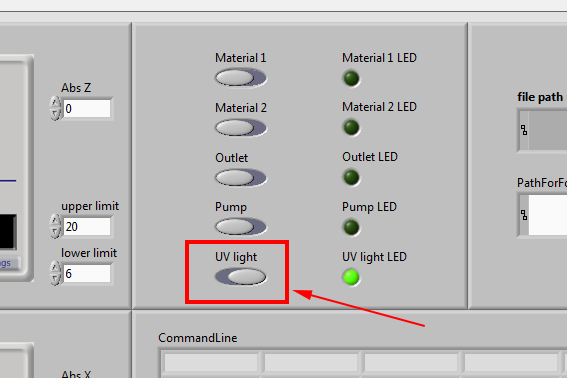
\includegraphics[width=0.4\textwidth]{step5_1.png}}
  &\raisebox{-\height}{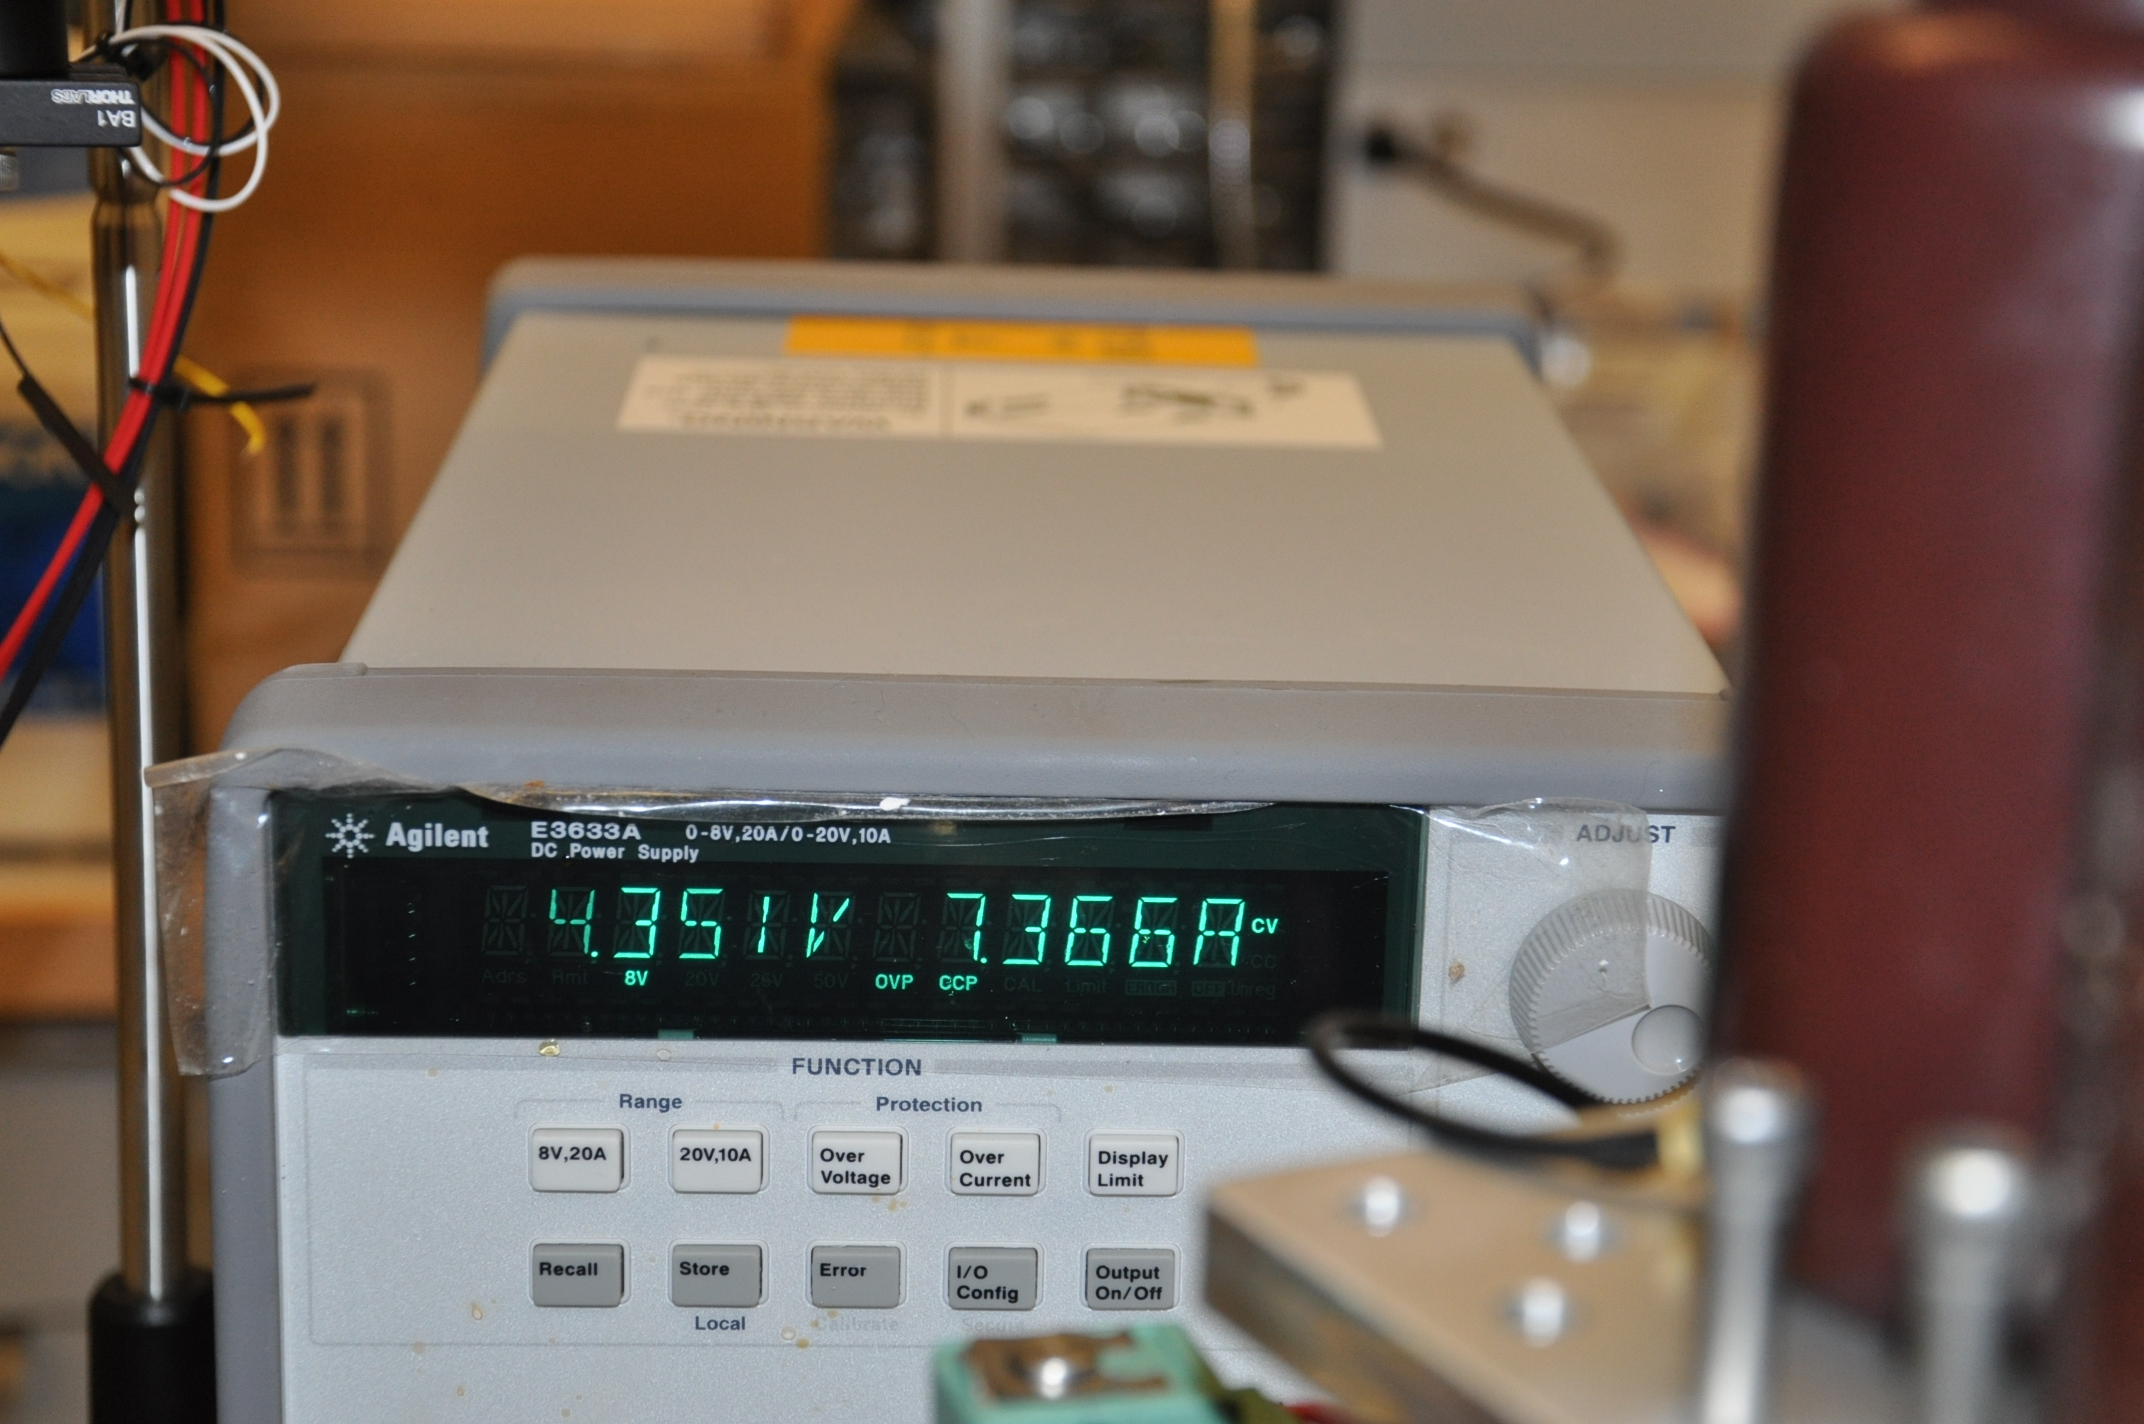
\includegraphics[width=0.4\textwidth]{step5_2.JPG}}
  \\
\end{tabularx}

The printing control part is used to set the root path of printing script and image. \underline{Remember to click refresh 
  when you have finished your settings and double check the \#total lines in the scripts}. \\ 
\textbf{Click} print to execute the printing.\\
When a script has been executed, \textbf{click} stop at the top left corner and \textbf{run} the \textit{Labview} again to 
begin another printing\\
\begin{tabularx}{\textwidth}{XX}
  \raisebox{-\height}{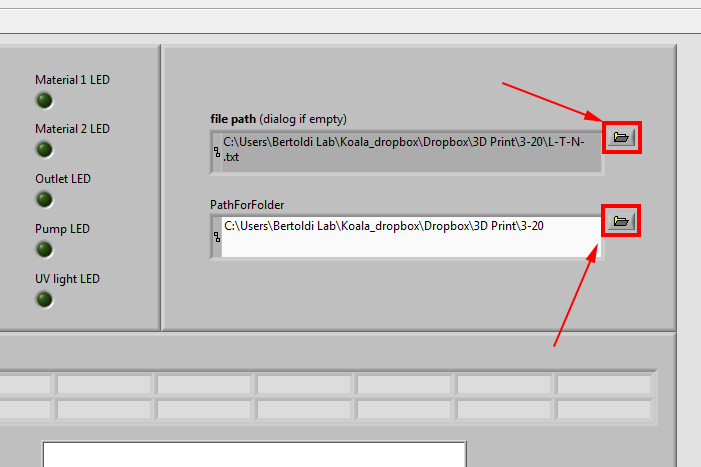
\includegraphics[width=0.4\textwidth]{script31.png}}
  &\raisebox{-\height}{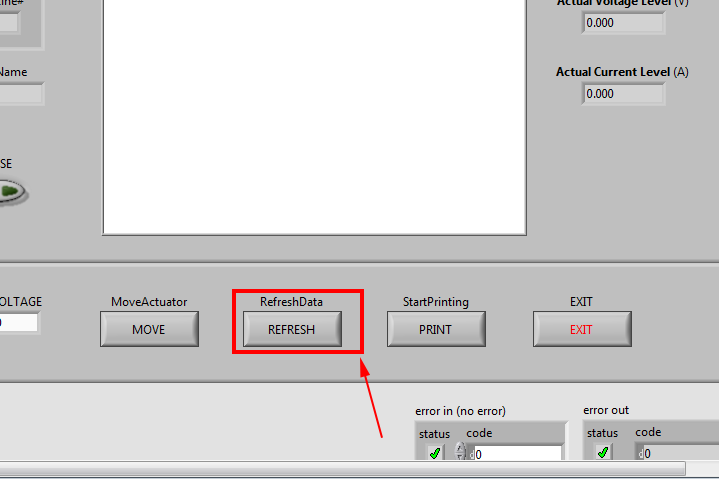
\includegraphics[width=0.4\textwidth]{script32.png}}
  \\
\end{tabularx}



\subsubsection{Runsheet}
% The tool to automatically generate the script used for 3D printing. \textbf{Type in} the parameters

(layers,exposure time etc) 
% and \textbf{click} create to produce the script under the \underline{same directory}.\\
% \textbf{(1)2D extrusion structure}:\\
% \textbf{Put} the 2D cross-section to be printed and the script under the \textbf{same catalogue} and 

\textbf{choose} the 
% correct path at the \textit{labview} printing control part. \\
% \textbf{(2)Arbitrary 3D struture}:\\
% \textbf{Slicing} the 3D structures into layers of 2D cross-section using \textit{CAD} and \textbf{name} 

them according to the 
% corresponding layer. For example, if there are a hundred 2D pictures which correspond to the cross-

sections of the 3D-structures, 
% from the first cross-section at the bottom and the hundredth cross-section at the very top. Then 

\textbf{name} the 100 pictures 
% from pic.1 to pic.100. \textbf{Put} the pictures and the script under the \underline{same directory}. 

\textbf{Choose} the right 
% path in the \textit{Labview} printing control part.
\textit{runsheet.py} on the desktop is used to generate the printing script. Double click the \textit

{runsheet.py}, then an 
user-interface will be shown on the screen. There are several parameters needed to be set:
\begin{tabularx}{\textwidth}{XX}
  \raisebox{-\height}{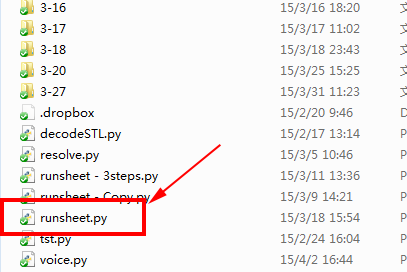
\includegraphics[width=0.4\textwidth]{step11.png}}
  &\raisebox{-\height}{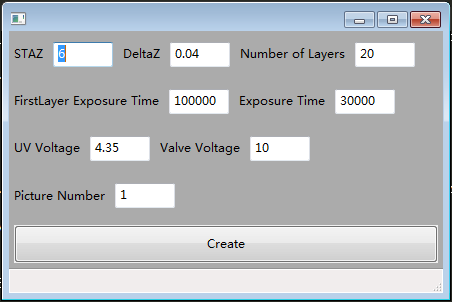
\includegraphics[width=0.4\textwidth]{runsheet_screenshot.png}}
  \\
\end{tabularx}
\begin{itemize}
  \item STAZ: It's the initial position of postion. the value of it should be set to \textit{initialZ} 

got from section 
  \ref{sec:printing preperation} step 7.
  \item DeltaZ: It's the thickness of each layer, which depends on your need. (unit: mm)
  \item Number of Layers: It determines the height of the whole sample with \textit{DeltaZ}. (unit: $\mu

$s)
  \item First layer exposure time: The first layer should be exposed to the UV Led source much longer, in 

order to ensure 
  that the sample can be bond well with the piston. (uint: ms)
  \item Exposure Time: Other layers's exposure time. (uint: ms)
  \item UV Voltage: It's the working voltage of the UV Led source. 4.35 shown on the picture is the 

maxium value, limited by the 
  power supply we use.  (uint: v)
  \item Value Voltage: It's the working voltage of the magnetic valve. Setting to 9 volts should works. 

But sometimes the valve 
  can not work at 9 volts, you should increase it a bit. Note that the maxium voltage is 12v. If it still 

doesn't work, 
  please replace the valve and try again.(uint: v)
  \item Picture Number: The picture you want to print should be named in this template: X\_0\_0\_0.png. 

Note that the X in the file 
  name is a number, and the picture is in png format. Then set this parameter to the number you name your 

picture as. 
\end{itemize}
After you fullfilling in all the parameters, just click the create button and a printing script will be 

generated automatically in 
the same folder as this \textit{runsheet.py} program. It's highly recommanded to create a new folder 

every time you print and put 
the script generated with the picture together into it.




\subsubsection{Script introduction}
The script is used to control the P$\mu$SL 3D printing process. Every line in the script stands for a 

certain operation of 
a certain device. Table \ref{table_script} shows the meaning of each colume. More details can be found in 

file \textit{CommandFormat.xlsx} 
with this manual. For example in line 18(underlined with red line) in \textit{Fig \ref

{script_screen_shot}}, the combination of 
the second and third column means that the target device to operate on is the \textit{UV LED}. Column 5 

means the execution value 
is 0, which equals to turning the \textit{UV LED} off. The Column 4 means the execution time, which 

indicates that the \textit{UV 
LED} should be off for 1.5 seconds.
\begin{table}
  \begin{center}
    \begin{tabular}{ | c | c | c | c | c |}
      \hline
      Column 1 & Column 2 & Column 3 & Column 4 & Column 5 \\
      \hline
      number&the target&the target&time&execution value\\
      \hline
    \end{tabular}
    \caption{the explanation of different columns in the script}\label{table_script}
  \end{center}
\end{table}
\begin{figure}
  \centering
  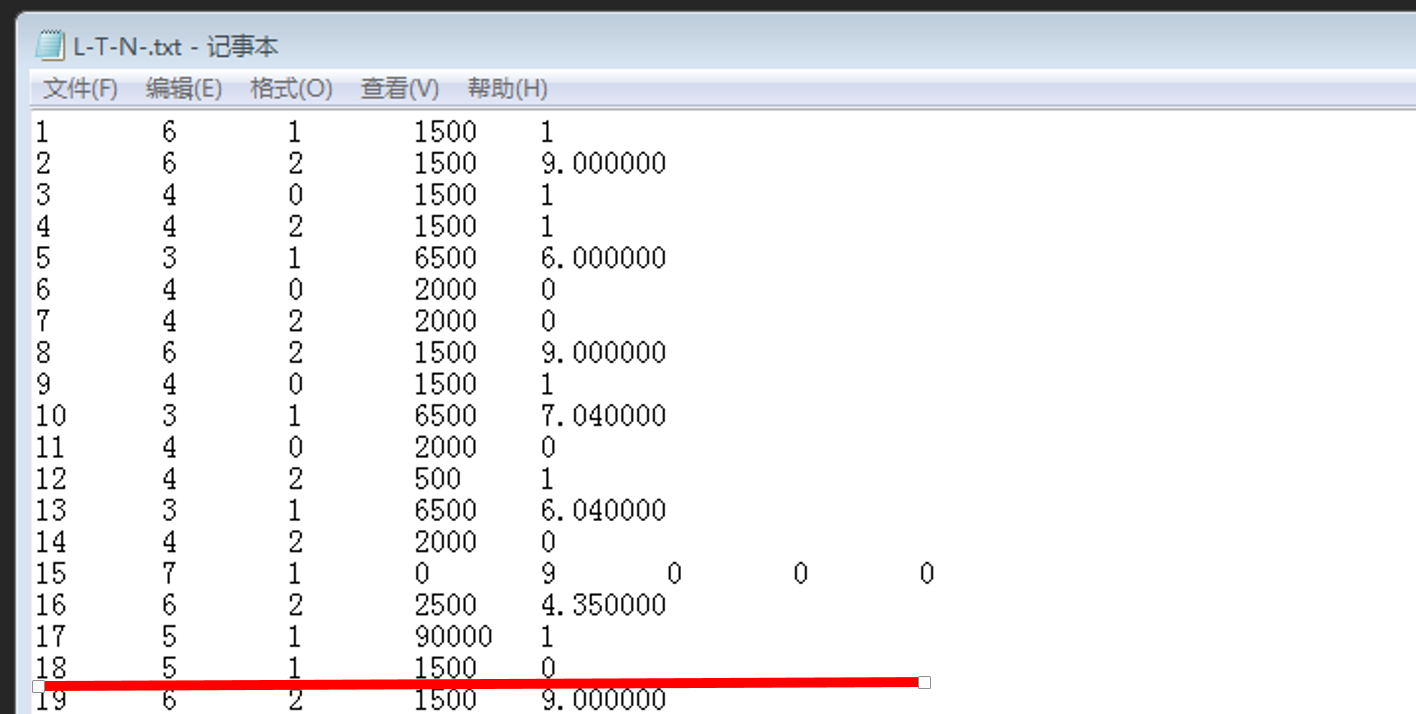
\includegraphics[width=0.7\textwidth]{script22.png}
  \caption{The script of P$\mu$SL 3D printing }\label{script_screen_shot}
\end{figure}
\clearpage





\section{Operation Procedure}\label{sec:page-layout}
In this section, the normal operation procedure of the 3d-printer will be introduced. Just follow the steps. \\
\underline {To your own safety, always wear gloves before doing anything and wash hands after experiments.}

\subsection{Printing preperation}\label{sec:printing preperation}
\begin{itemize} %圆点提示符号
  \begin{tabularx}{\textwidth}{ XXX } 
  \item \textbf{Step 1} : \textbf{Turn on} the \textit{power strip} on the ground. \textbf{make sure} the \textit{fan} 
    behind the \textit{UV Light} function well before \textbf{turning on} the \textit{projector}, \textit{lightsource}, 
    \textit{ computer} and \textit{power source} in sequence.
    &\raisebox{-\height}{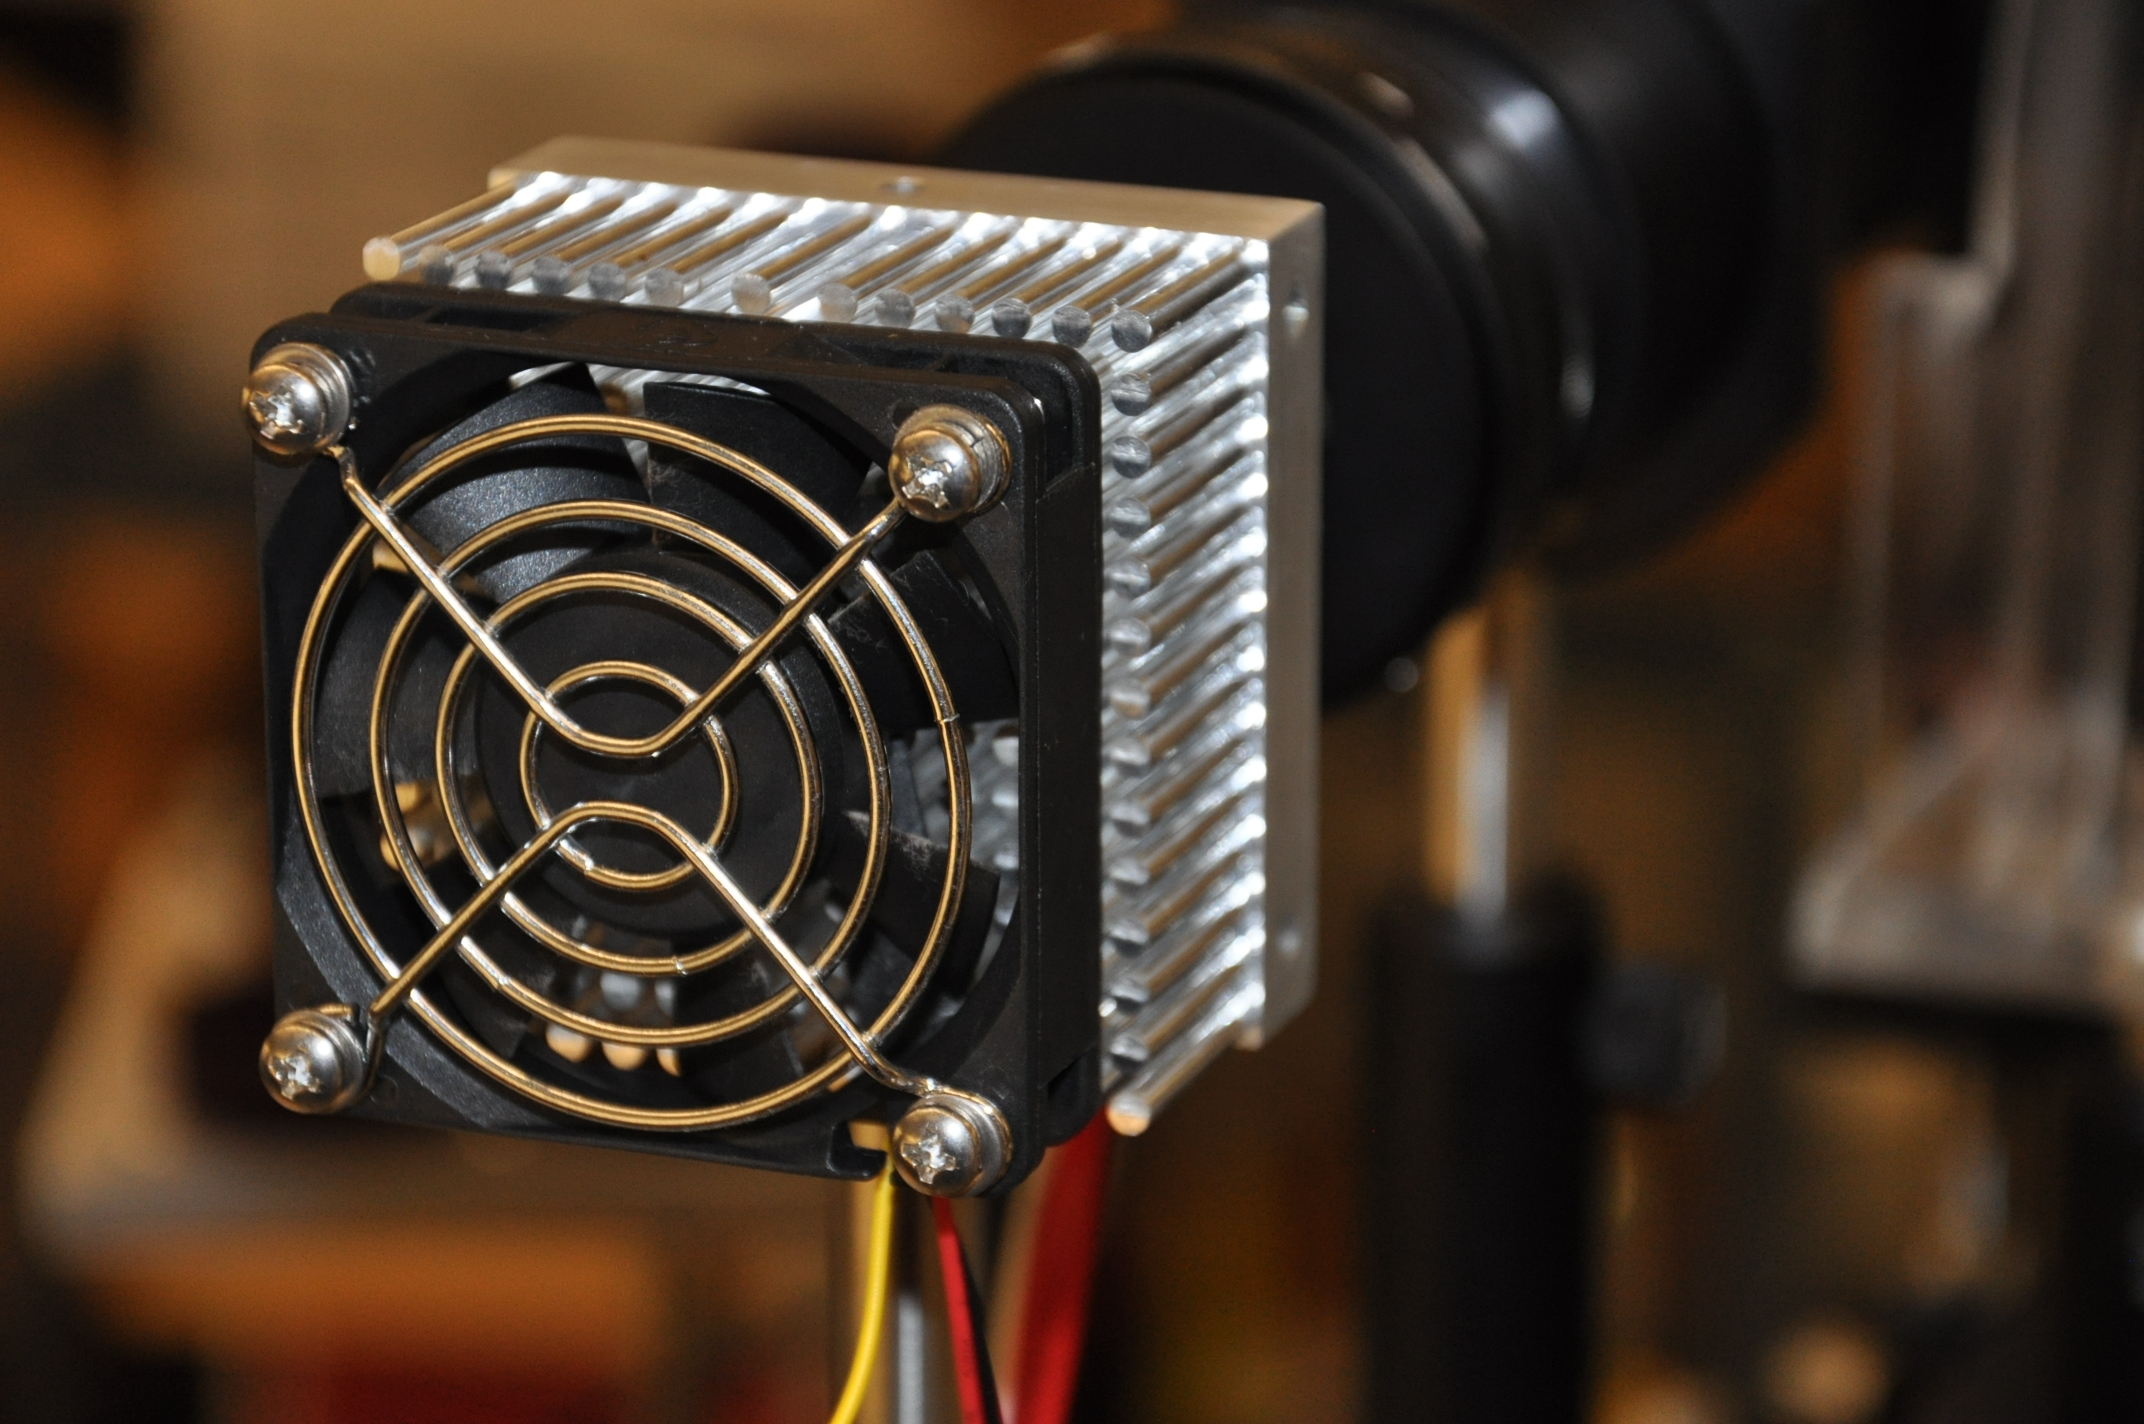
\includegraphics[width=0.3\textwidth]{step_1_fan.JPG}}
    &\raisebox{-\height}{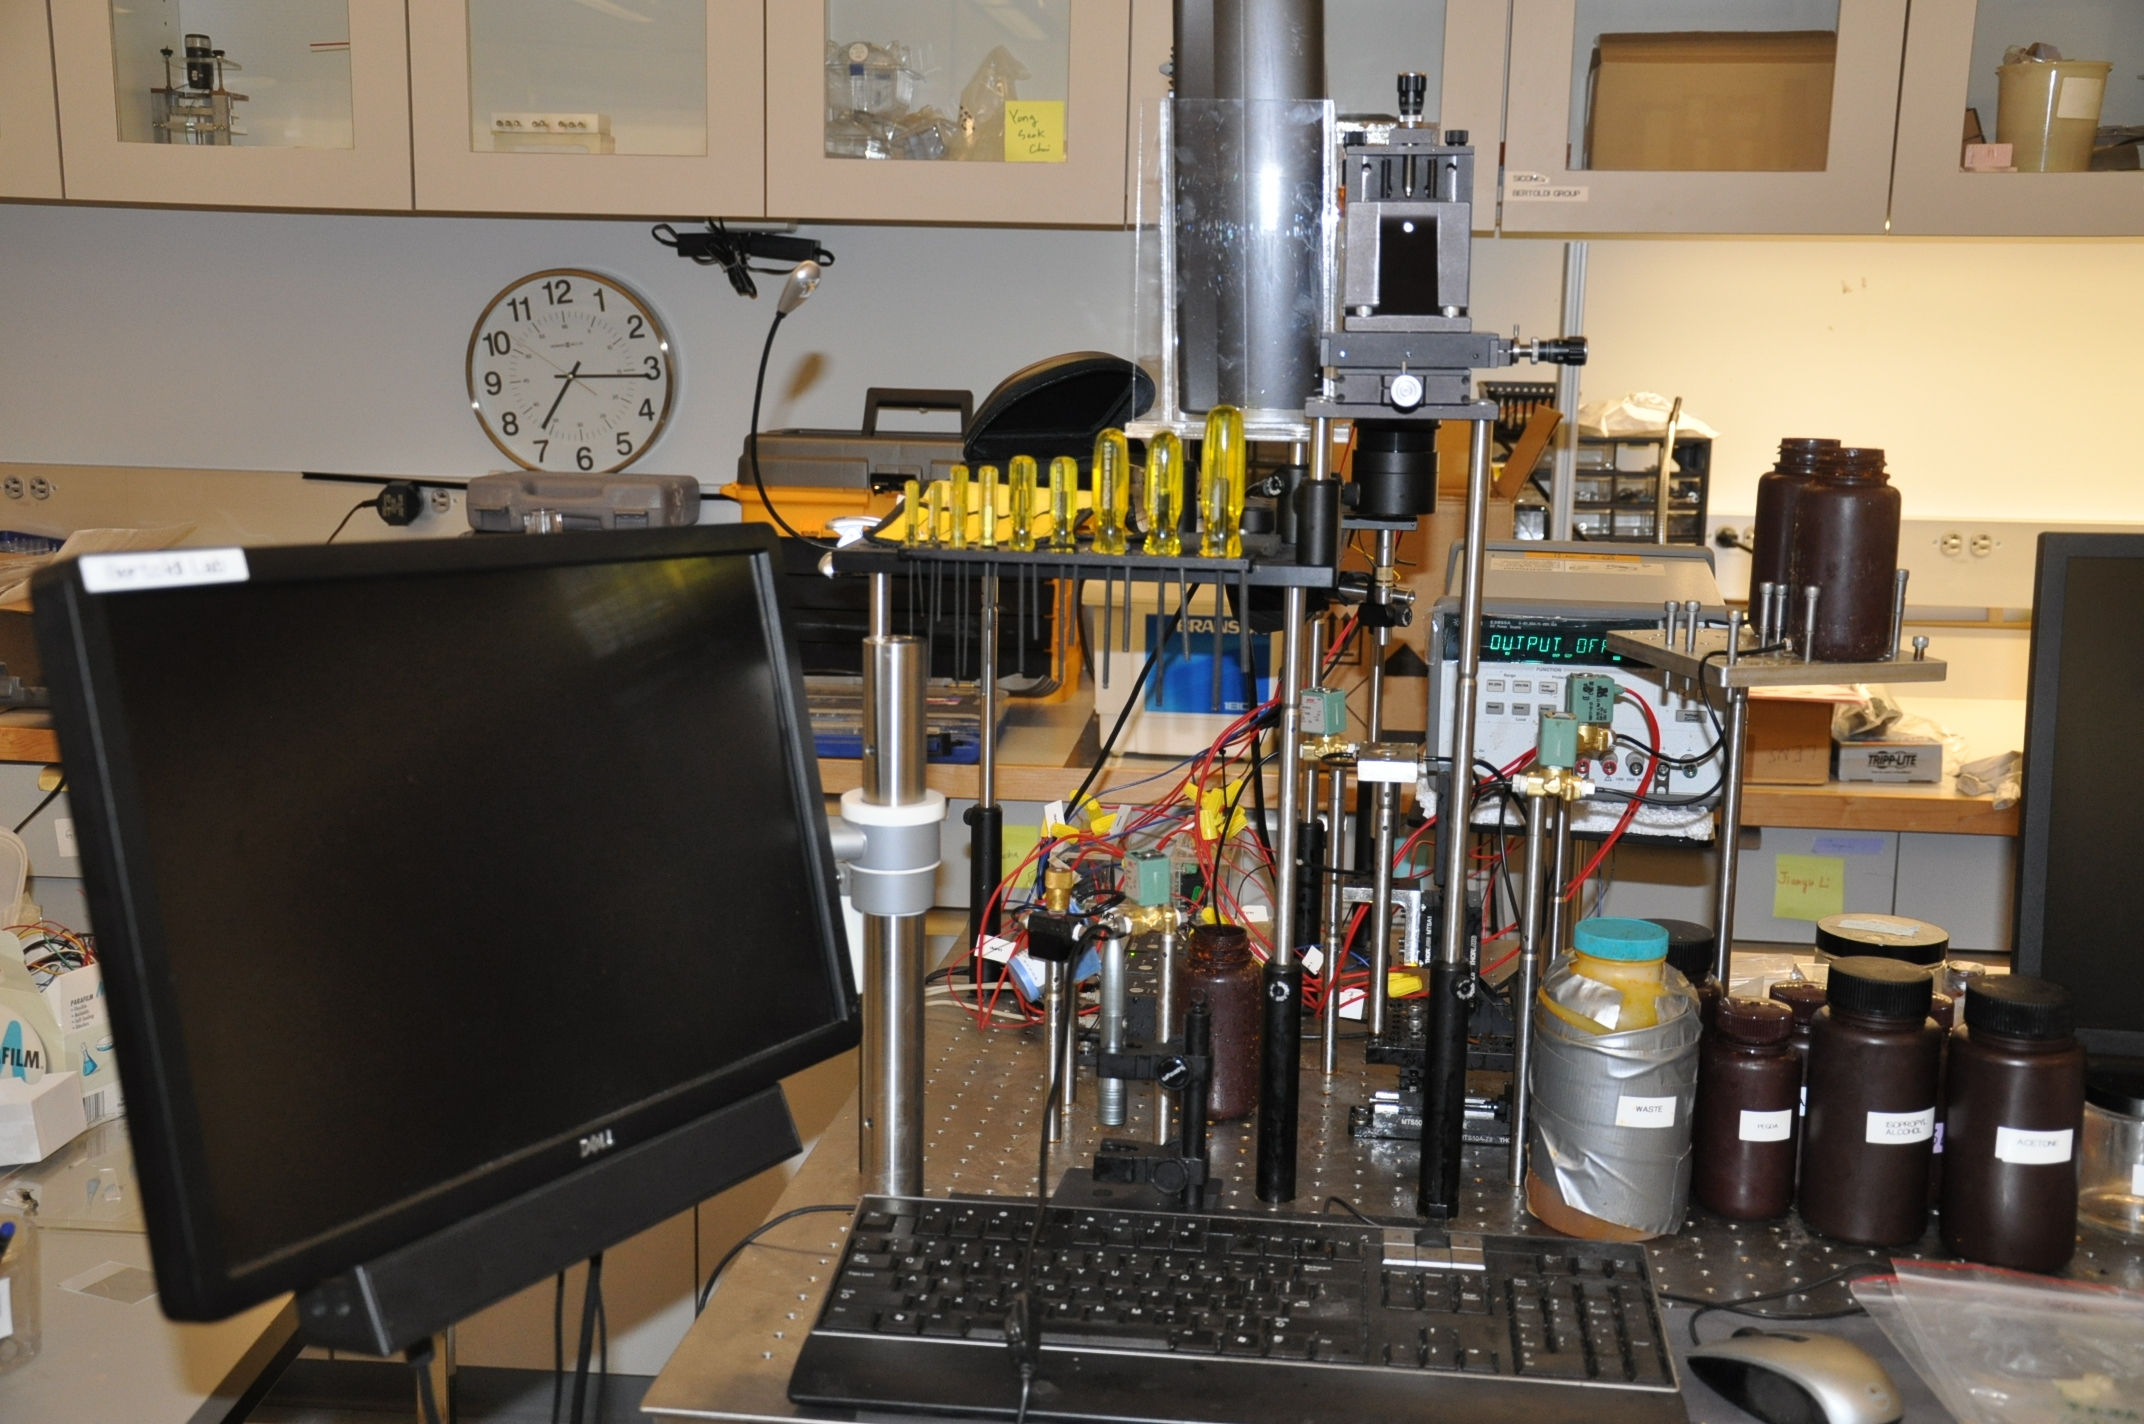
\includegraphics[width=0.3\textwidth]{step_1_overview.JPG}}\\
  \end{tabularx}

  \begin{tabularx}{\textwidth}{ XXX }
  \item \textbf{Step 2} : \textbf{Open} \emph{Labview} at the desktop and \textbf{click} \emph{main.vi}. After the interface 
    pops out, \textbf{click} the \textit{run} icon at the top left corner and \textbf{wait} for the pre-running self-check to 
    be completed.When the initialization is done, you will see parameters in green and red appear at the left side of the 
    interface.
    &\raisebox{-\height}{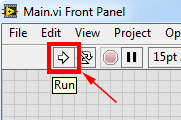
\includegraphics[width=0.3\textwidth]{step2_1.png}}
    &\raisebox{-\height}{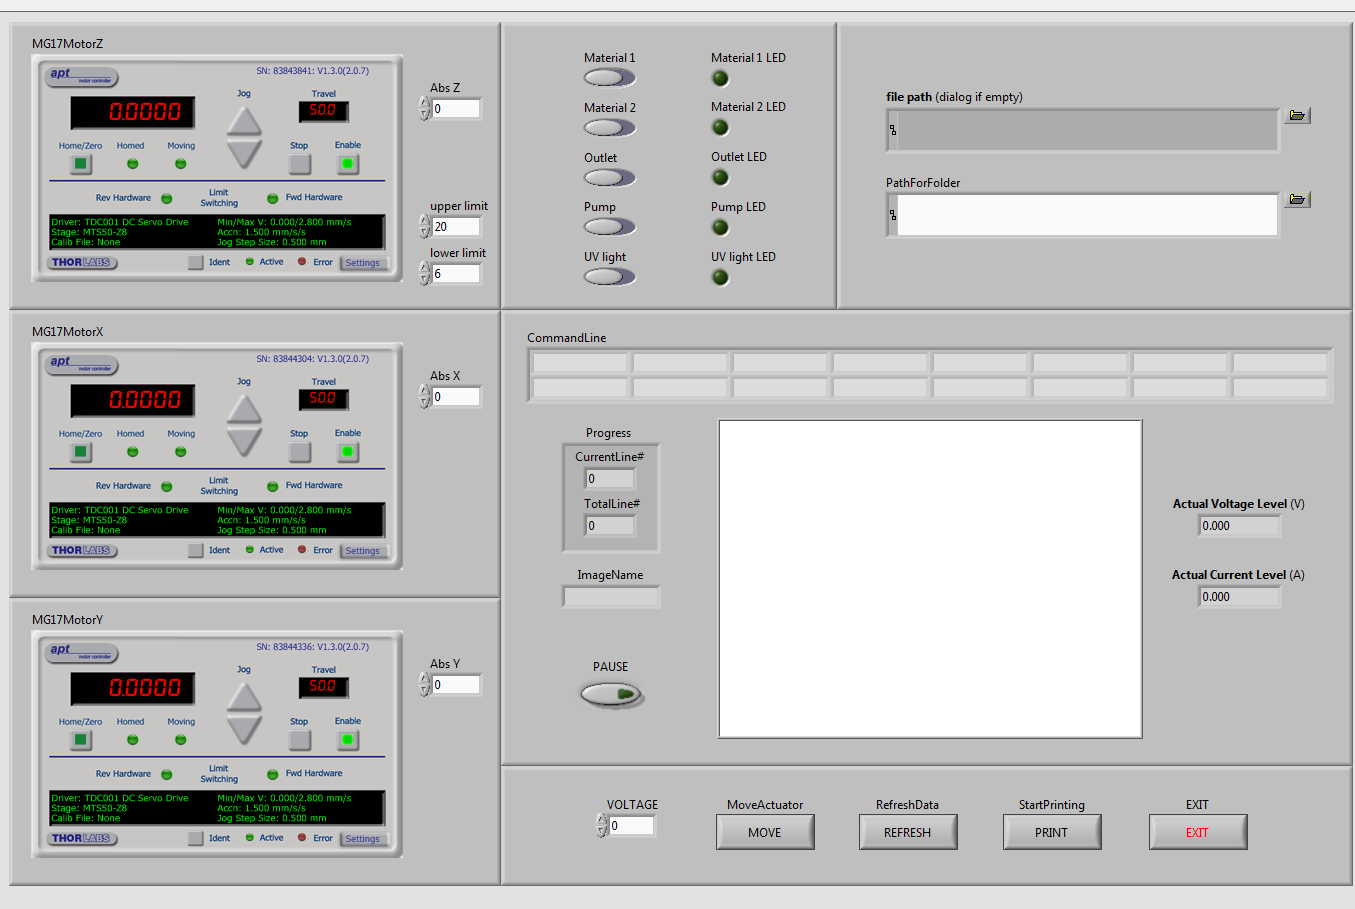
\includegraphics[width=0.3\textwidth]{step2_2.png}}\\
  \end{tabularx}

  \begin{tabularx}{\textwidth}{ XXX }
  \item \textbf{Step 3} :  \textbf{Return} the \textit{piston} to zero by \textbf{clicking} the home button.\textbf{Wait} 
    until the z-axis position is reset to zero.(\emph{\large{Only the z axis!!never home x or y axis}})
    &\raisebox{-\height}{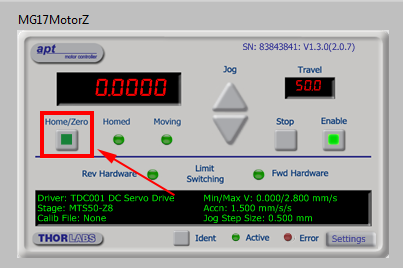
\includegraphics[width=0.3\textwidth]{step3_1.png}}
    &\raisebox{-\height}{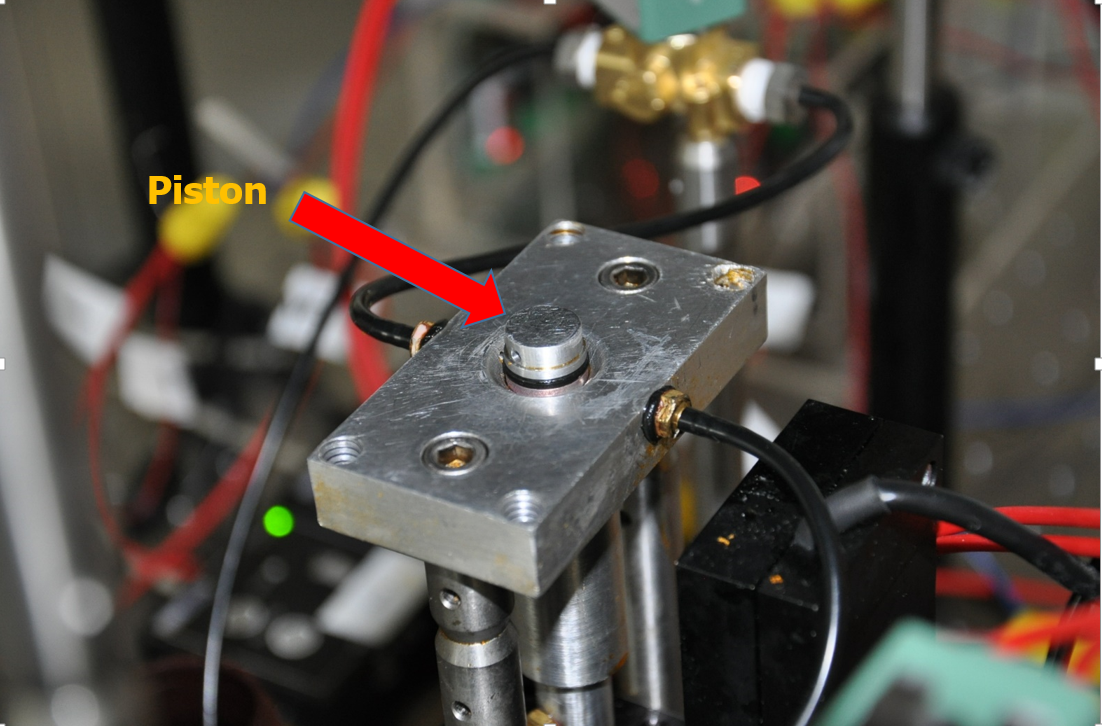
\includegraphics[width=0.3\textwidth]{step3_2.JPG}}\\
  \end{tabularx}
  
  \begin{tabularx}{\textwidth}{ XXX }
  \item \textbf{Step 4} :  \textbf{Click} setting icon and \textbf{change} the parameter of \textit{z-axis} movement of the 
    piston.(\textit{velocity, jogging distance,acceleration etc}). \textbf{See} 1.2 for \textbf{parameter details}.
    &\raisebox{-\height}{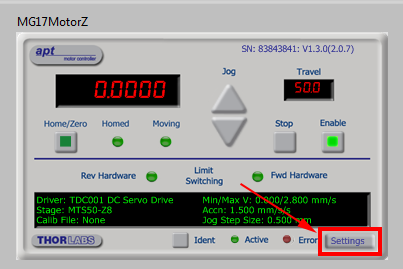
\includegraphics[width=0.3\textwidth]{step4_1.png}}
    &\raisebox{-\height}{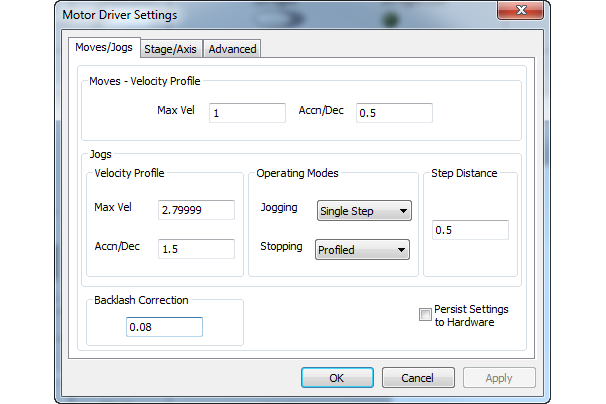
\includegraphics[width=0.3\textwidth]{step4_2.png}}\\
  \end{tabularx}

  \begin{tabularx}{\textwidth}{ XXX }
  \item \textbf{Step 5} :  \textbf{Click} the \textit{UV Light} button to \textbf{turn it on}. \textbf{Check} the screen 
    display of the \textit{power supply} and \textbf{make sure} the voltage output is below 4.35V.
    &\raisebox{-\height}{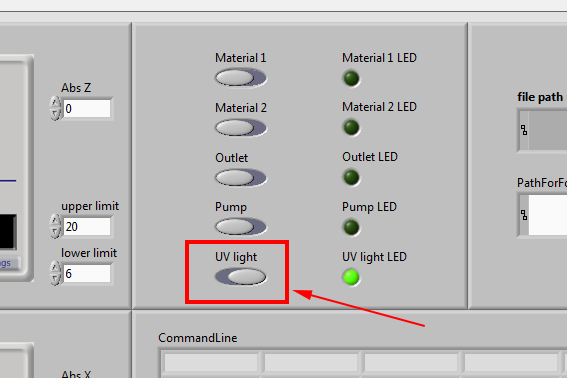
\includegraphics[width=0.3\textwidth]{step5_1.png}}
    &\raisebox{-\height}{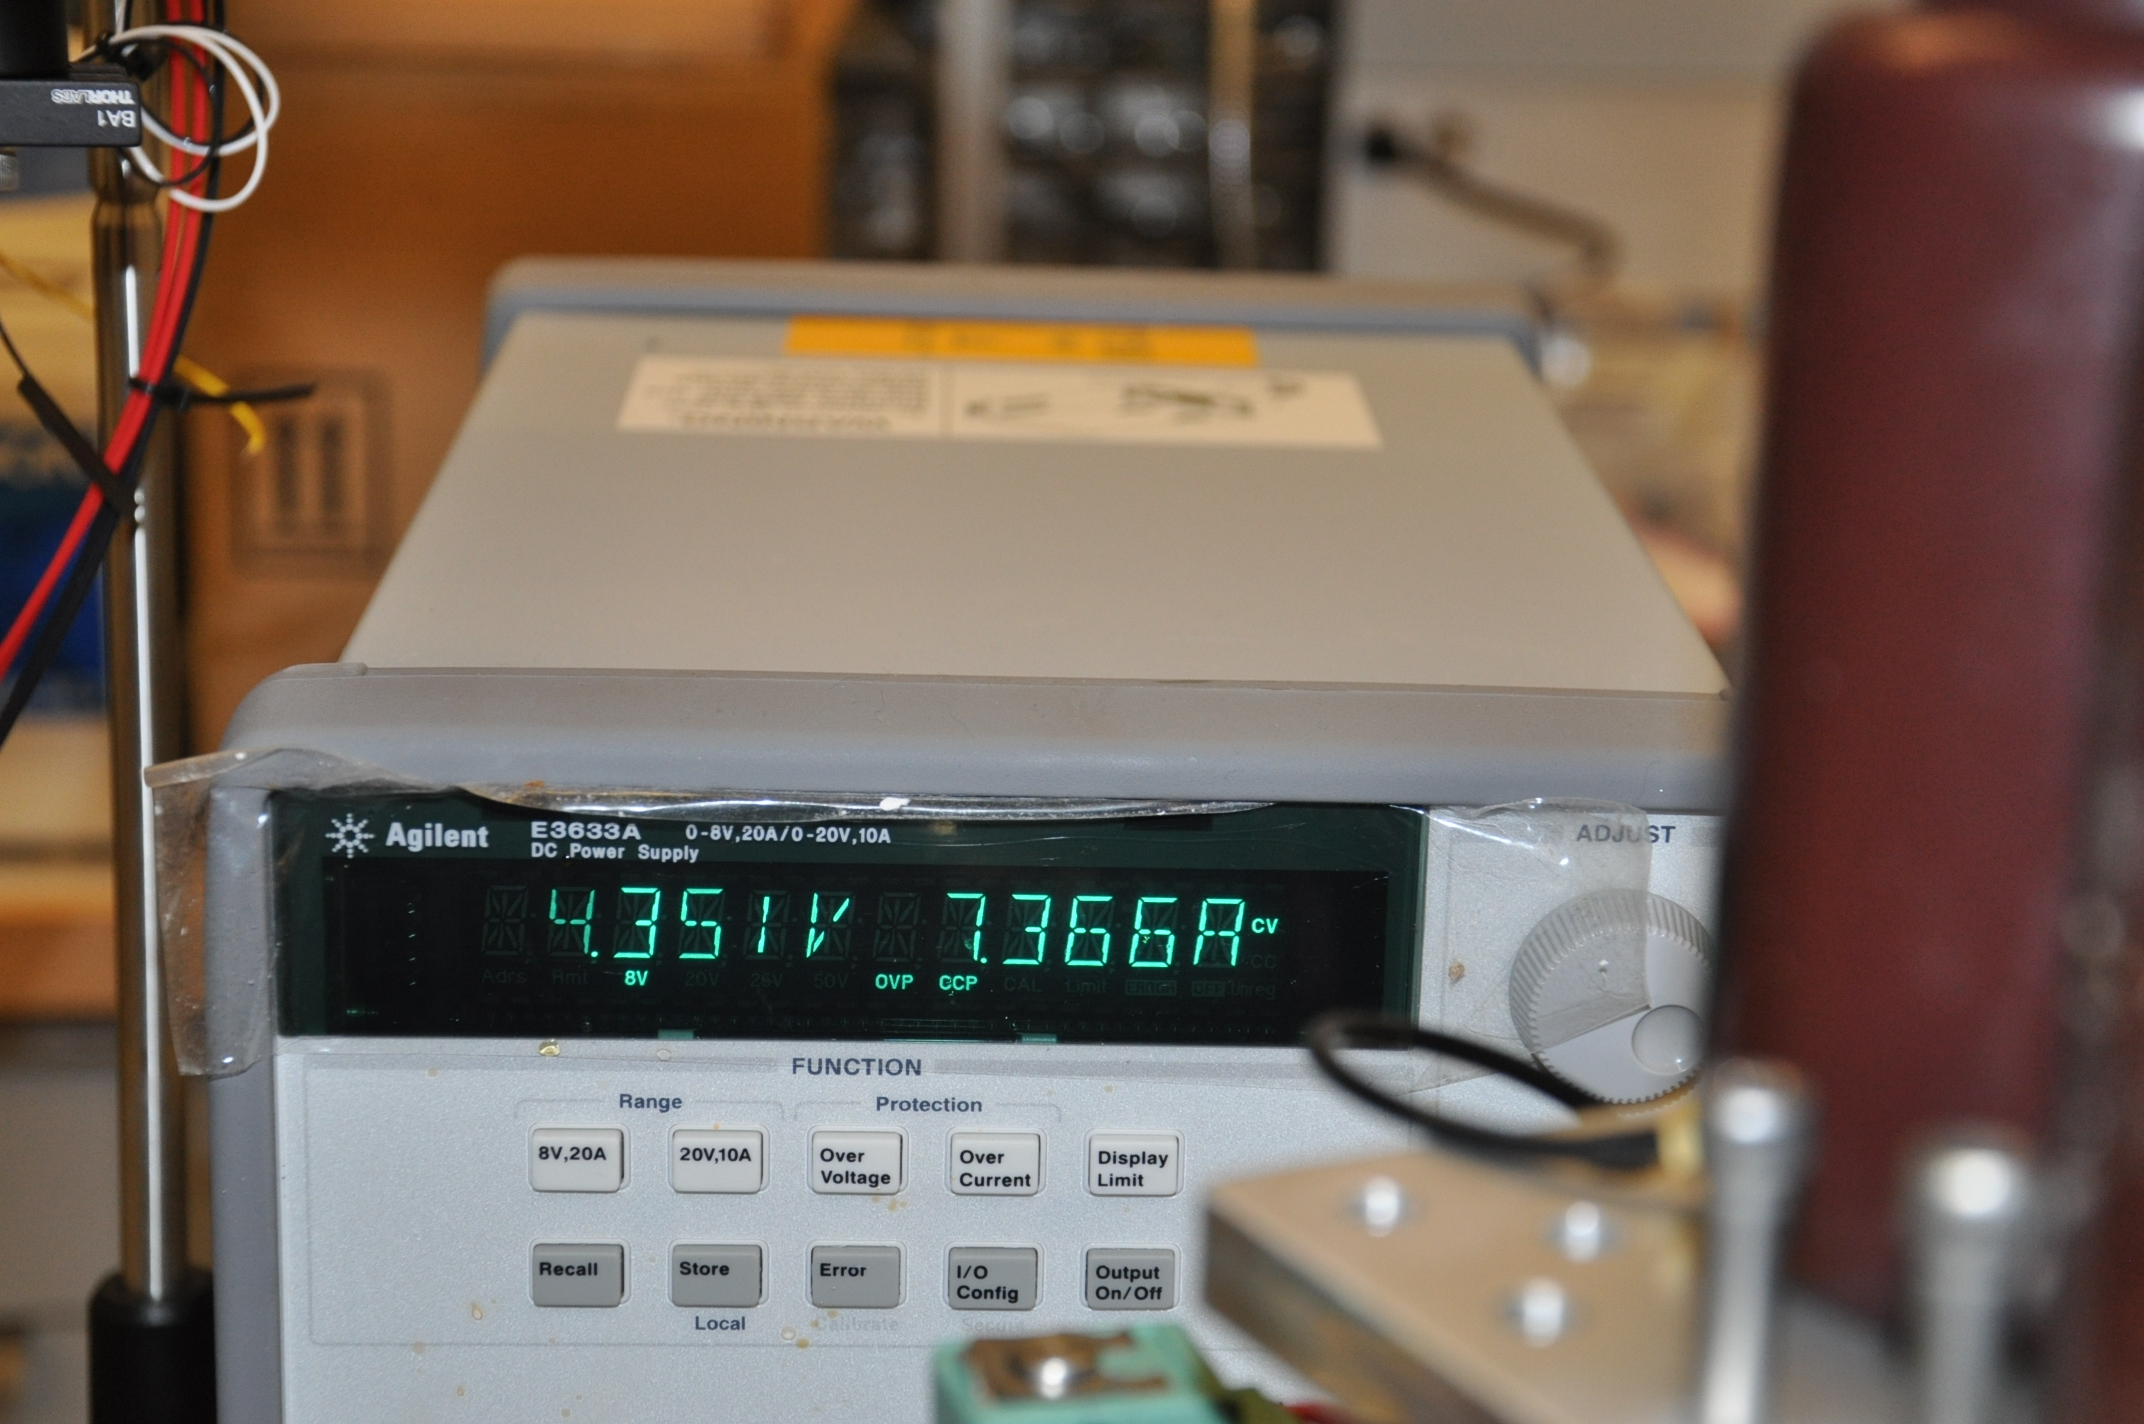
\includegraphics[width=0.3\textwidth]{step5_2.JPG}}\\
  \end{tabularx}

  \begin{tabularx}{\textwidth}{ XXX }
  \item \textbf{Step 6}:\textbf{Lower} the piston back to 7mm.\textbf{Put} a piece of paper on the \textit{motorized piston} 
    to \textbf{check} the precision of projected image.  
    The trick is: White paper is recommended for direct observation while black paper is preferred under \textit{Supereye} 
    microscope. If the projected image is not clear, \textbf{See} \textit{Appendix 3.2.2} for solution.
    &\raisebox{-\height}{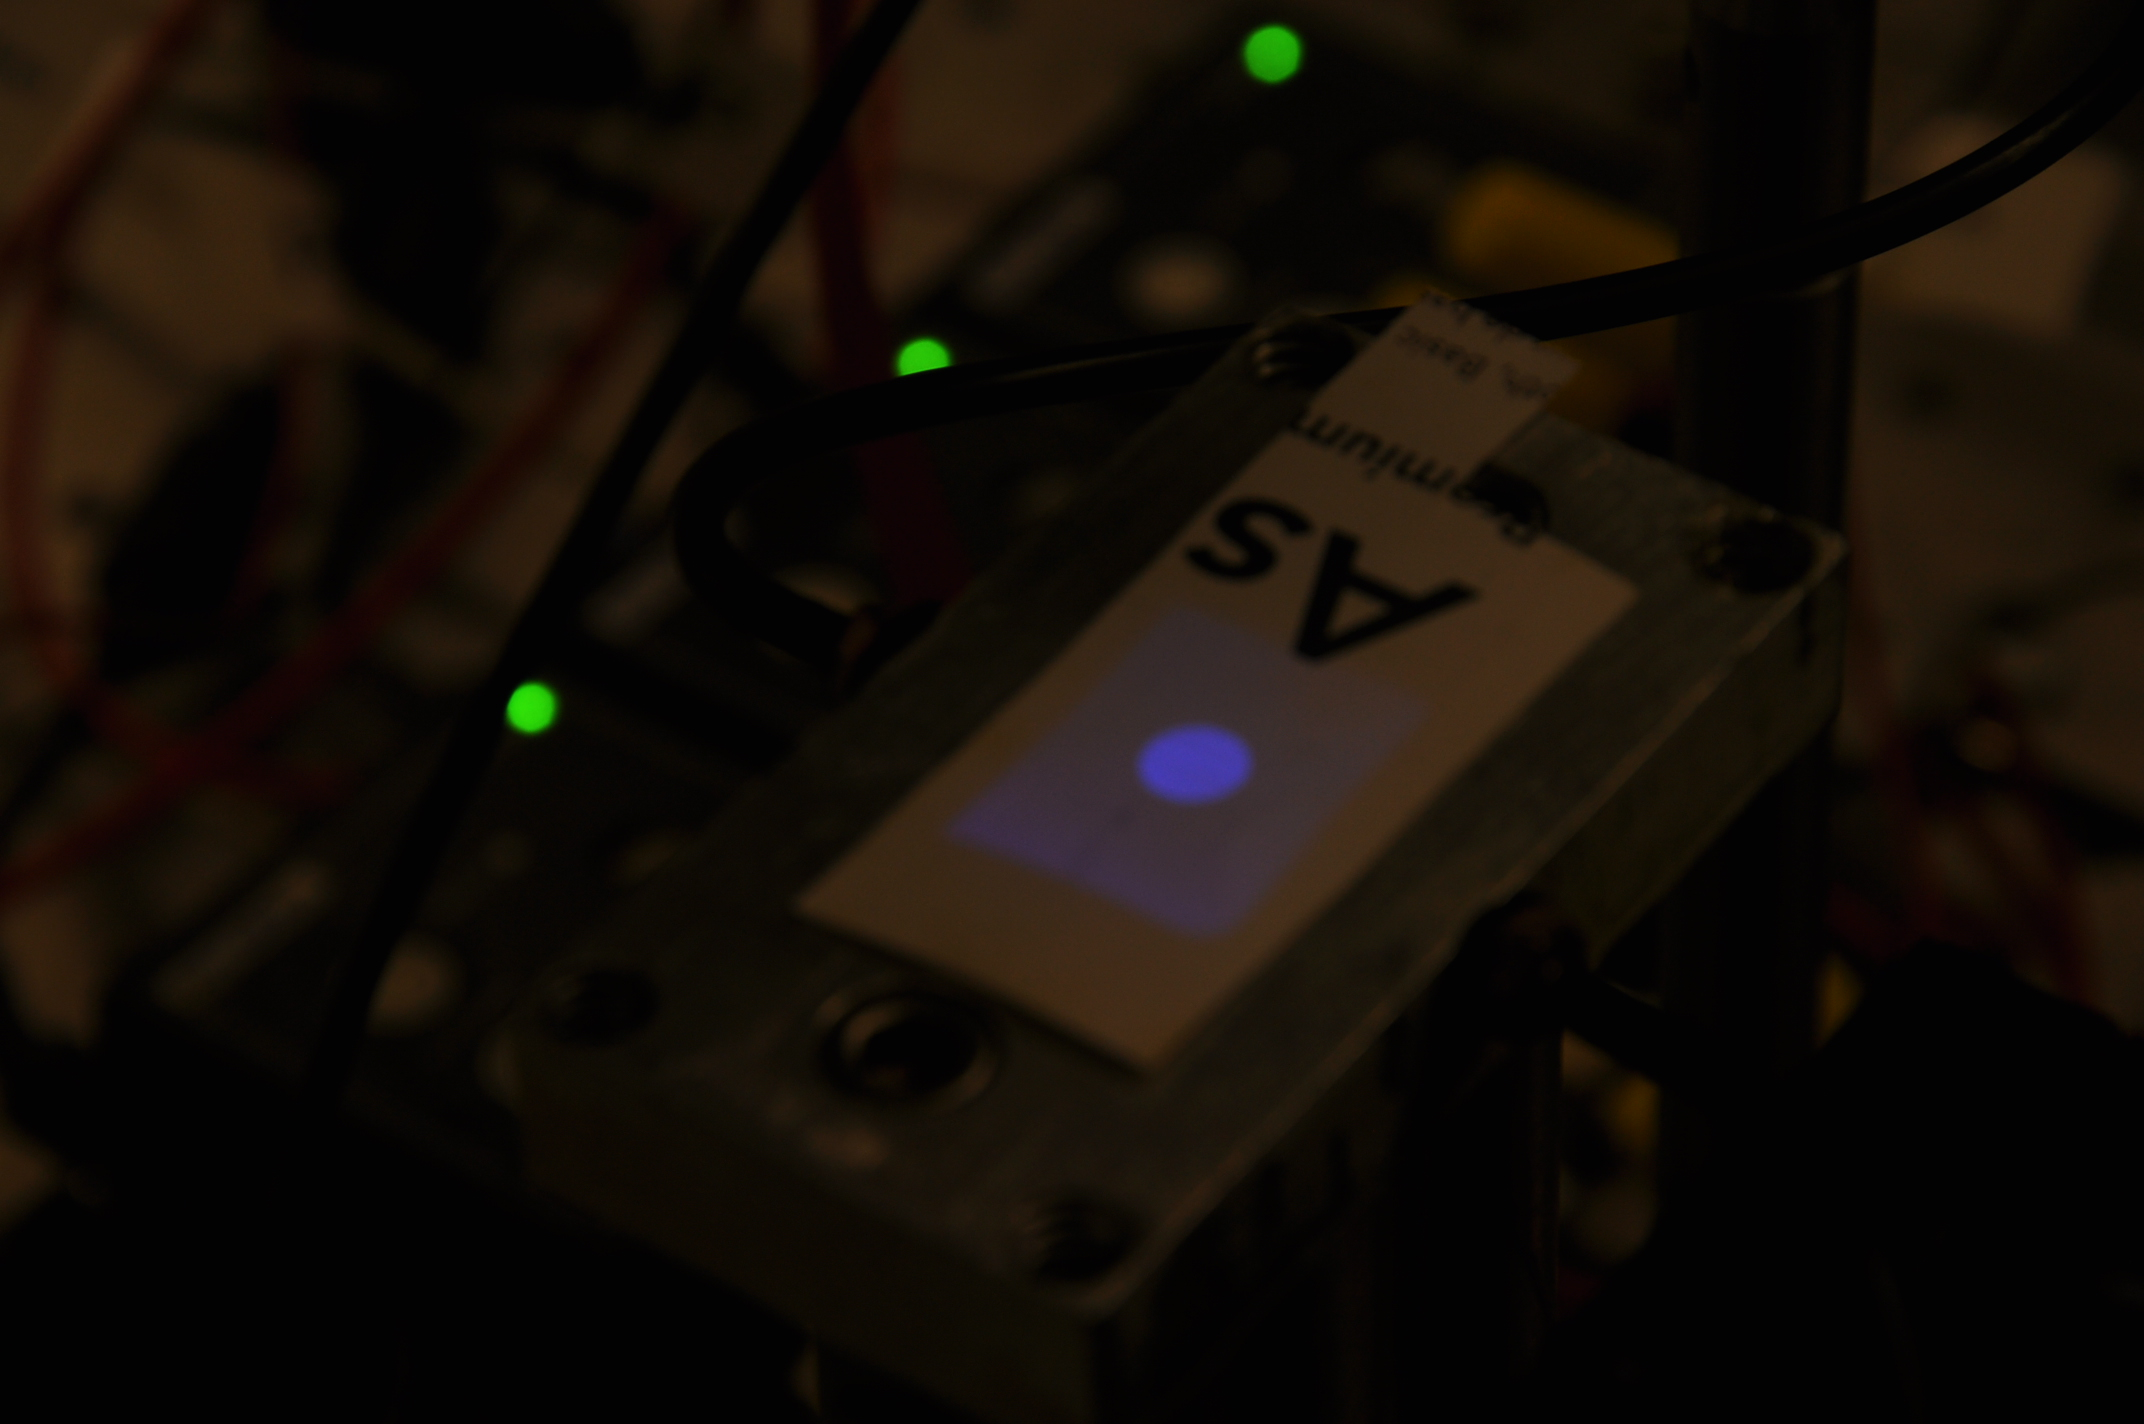
\includegraphics[width=0.3\textwidth]{step5_white.JPG}}
    &\raisebox{-\height}{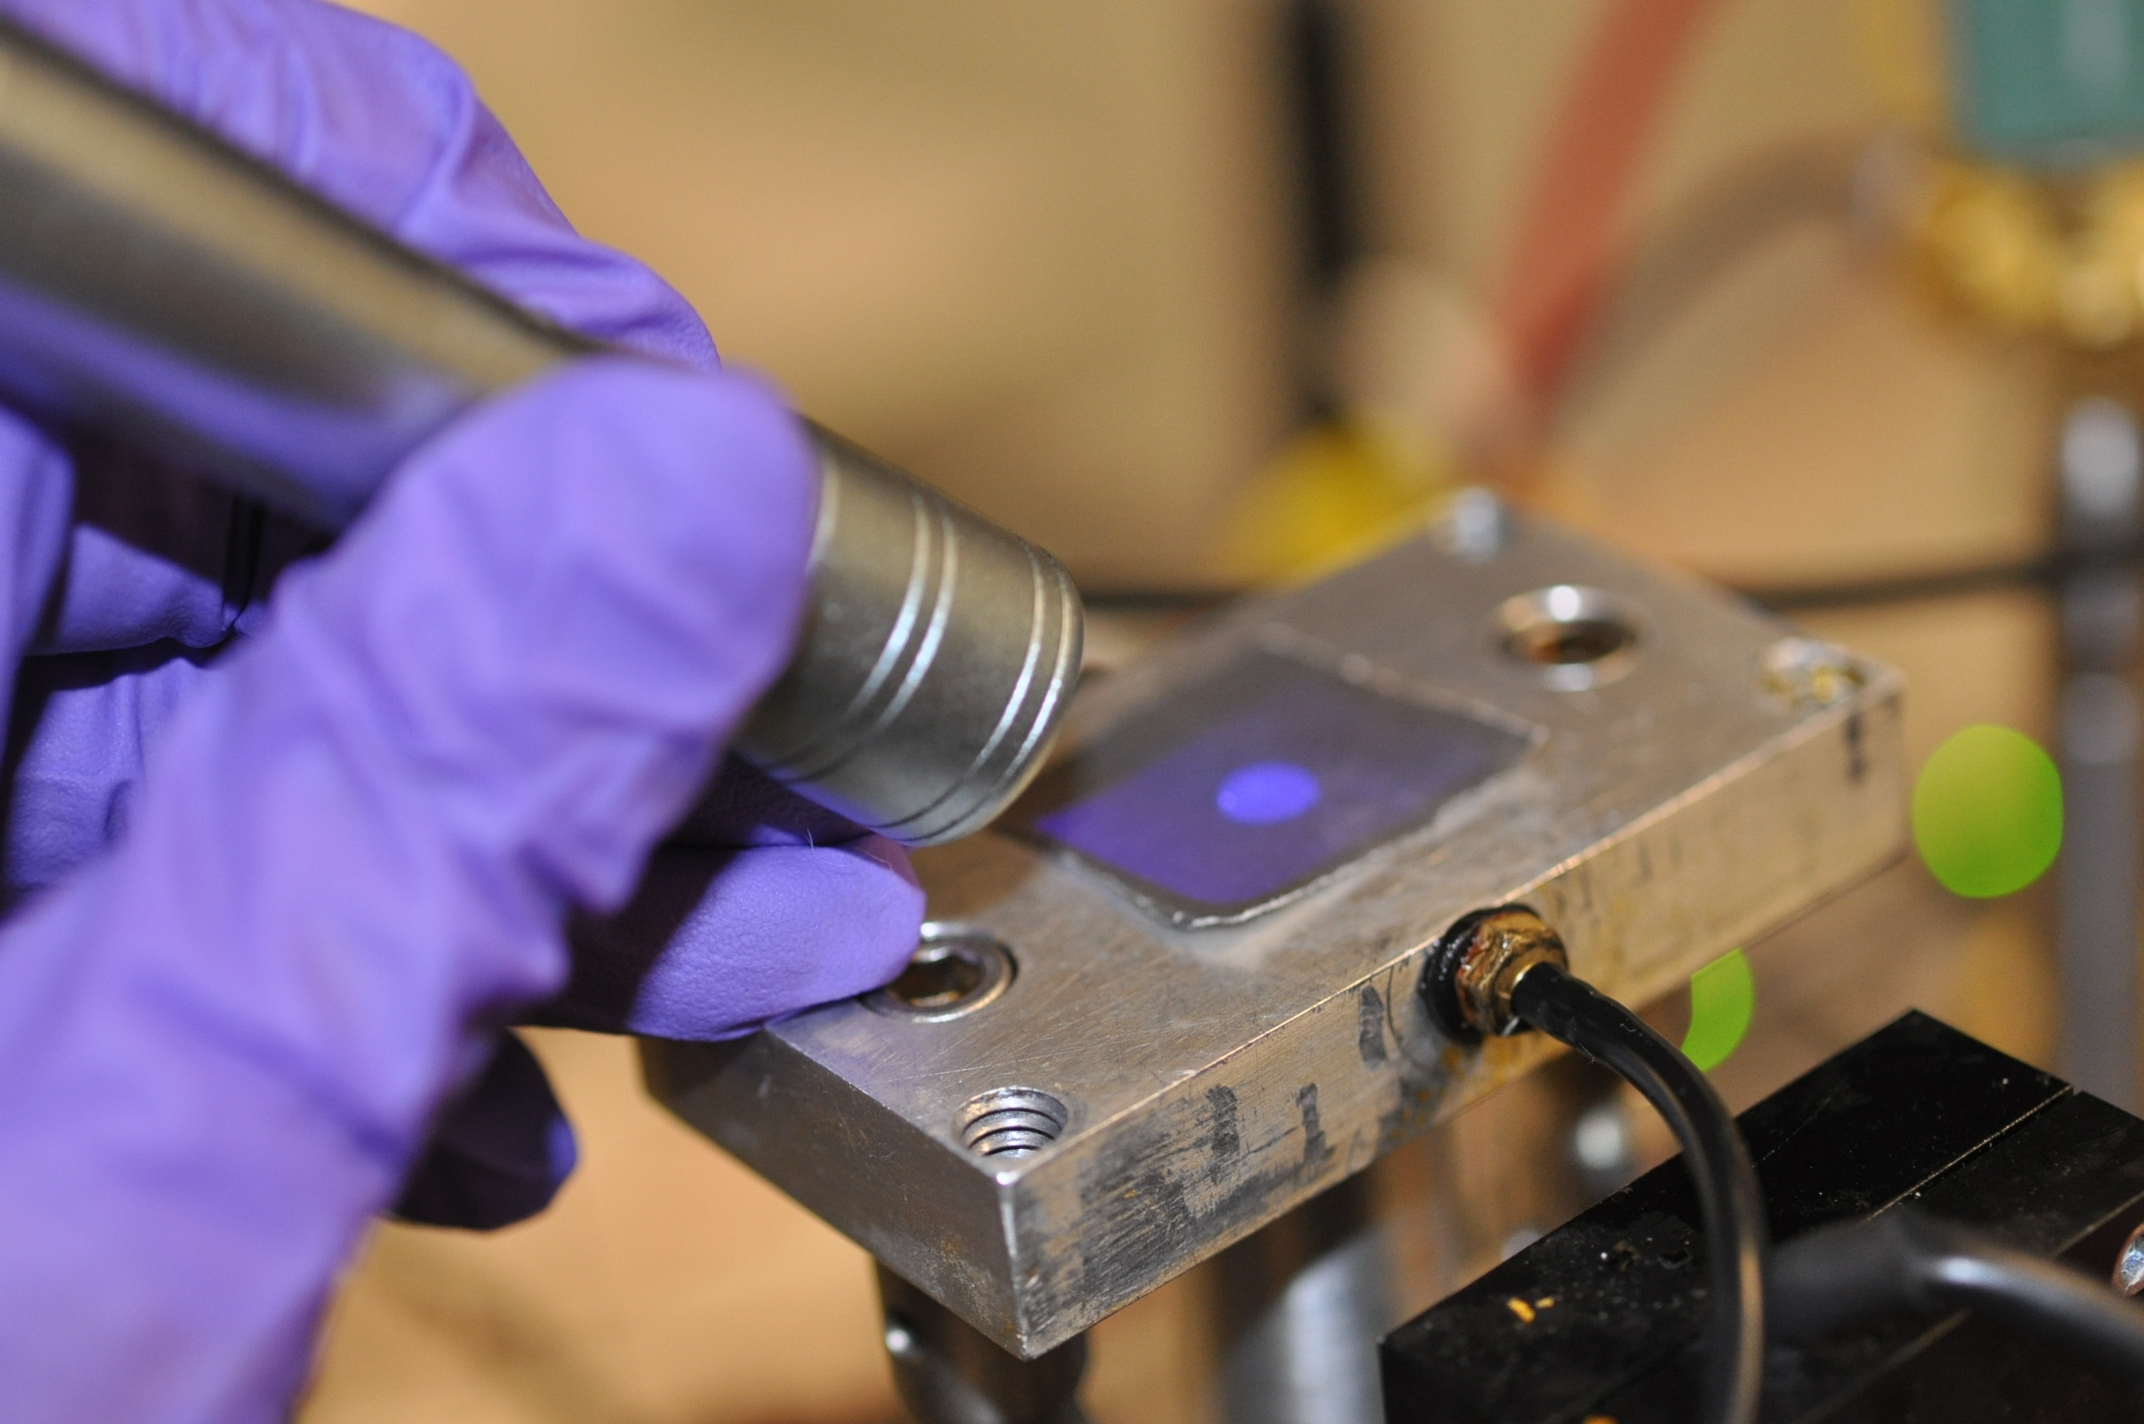
\includegraphics[width=0.3\textwidth]{step5_black.JPG}}
    \\
  \end{tabularx} \label{step 6}

  %		  \begin{tabularx}{\textwidth}{ XXX }
  %		   \item \textbf{Step 6}:\textbf{Rotate} the \textit{aperture} to 1.5
  %		   &\raisebox{-\height}{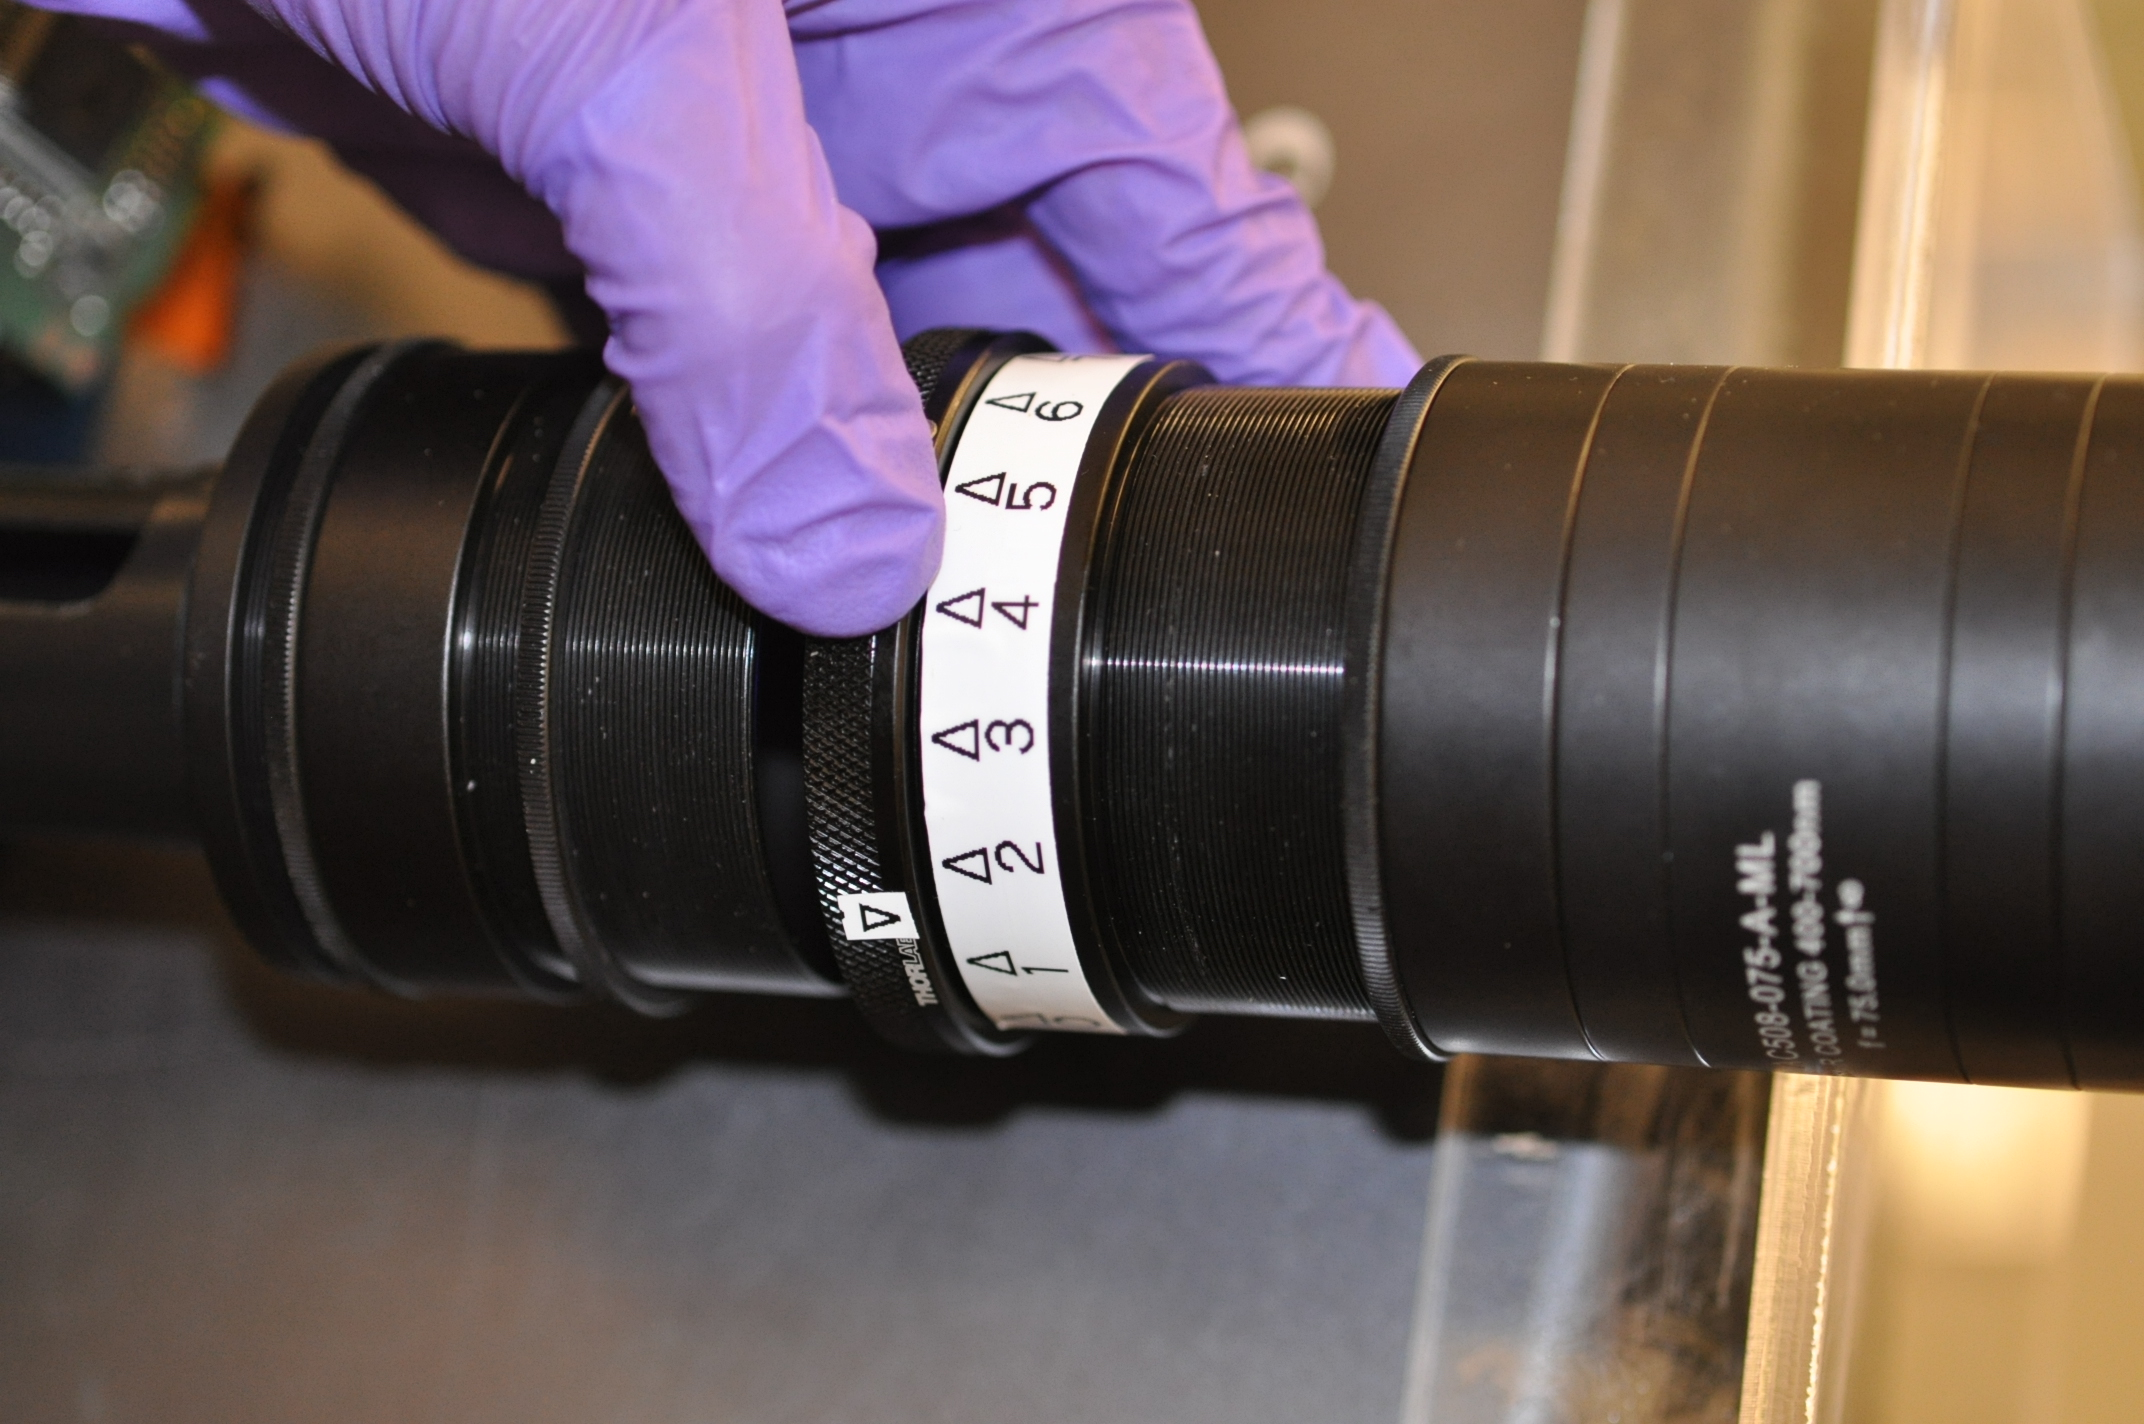
\includegraphics[width=0.3\textwidth]{step6_rotate.JPG}}
  %		   &\raisebox{-\height}{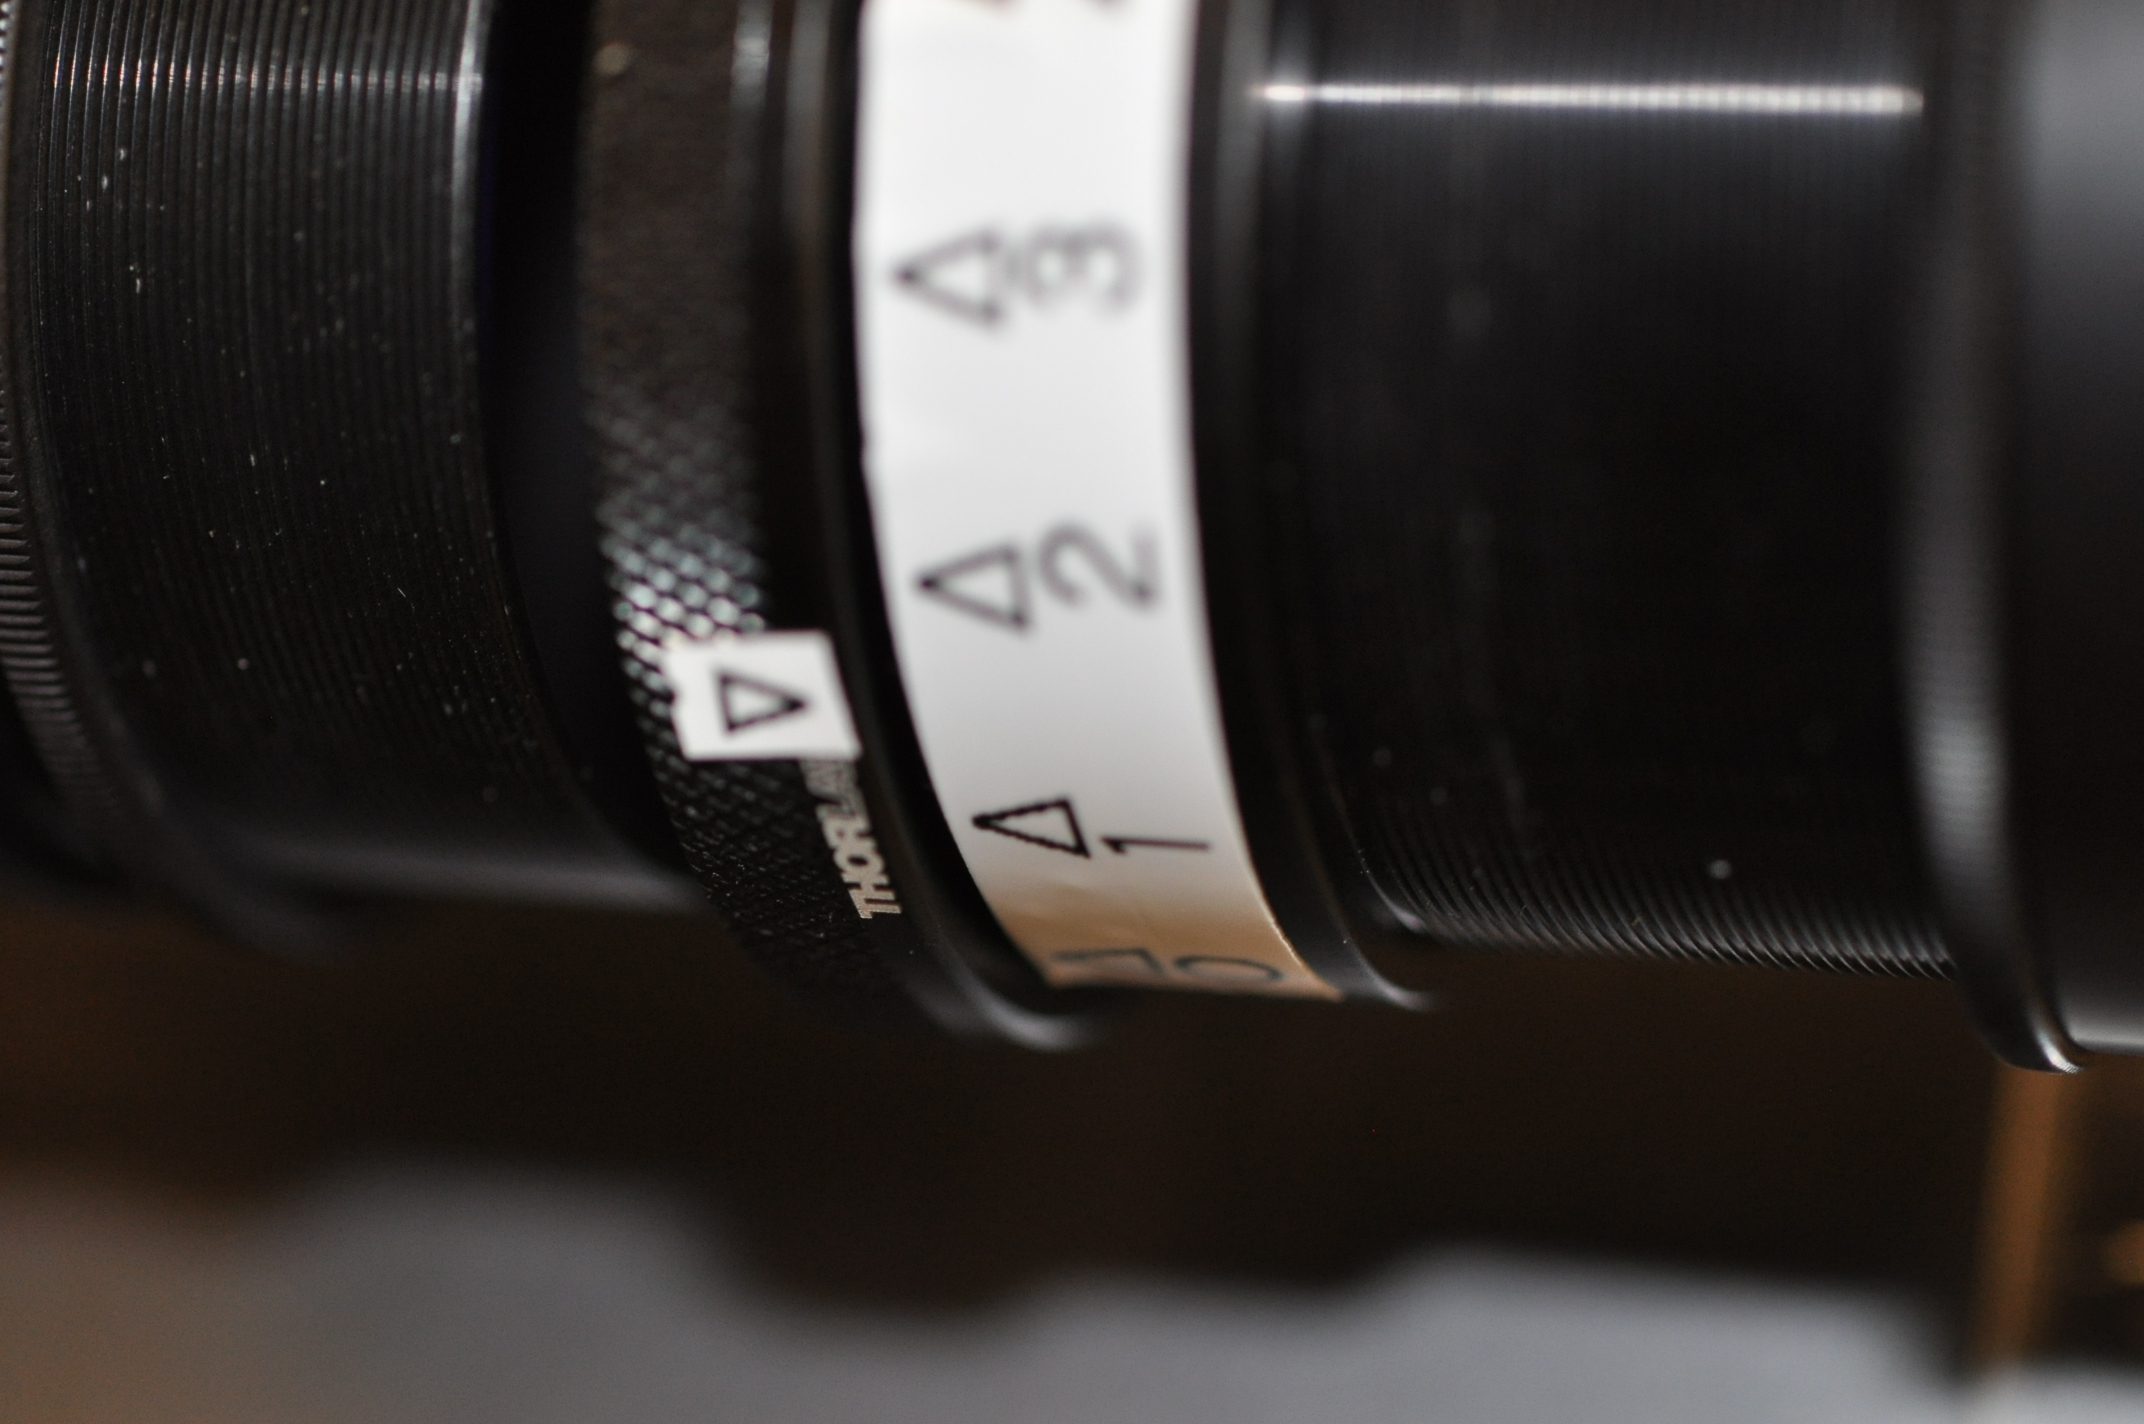
\includegraphics[width=0.3\textwidth]{step6_position.JPG}}\\
  %		   \\
  %		  \end{tabularx}
  
  \begin{tabularx}{\textwidth}{ XXX }
  \item \textbf{Step 7}:\textbf{Remove} the paper. \textbf{Use} a \textit{blade} to find the \emph{initial Z} for                    printing following the steps in \textit{Appendix} 3.1 
    &\raisebox{-\height}{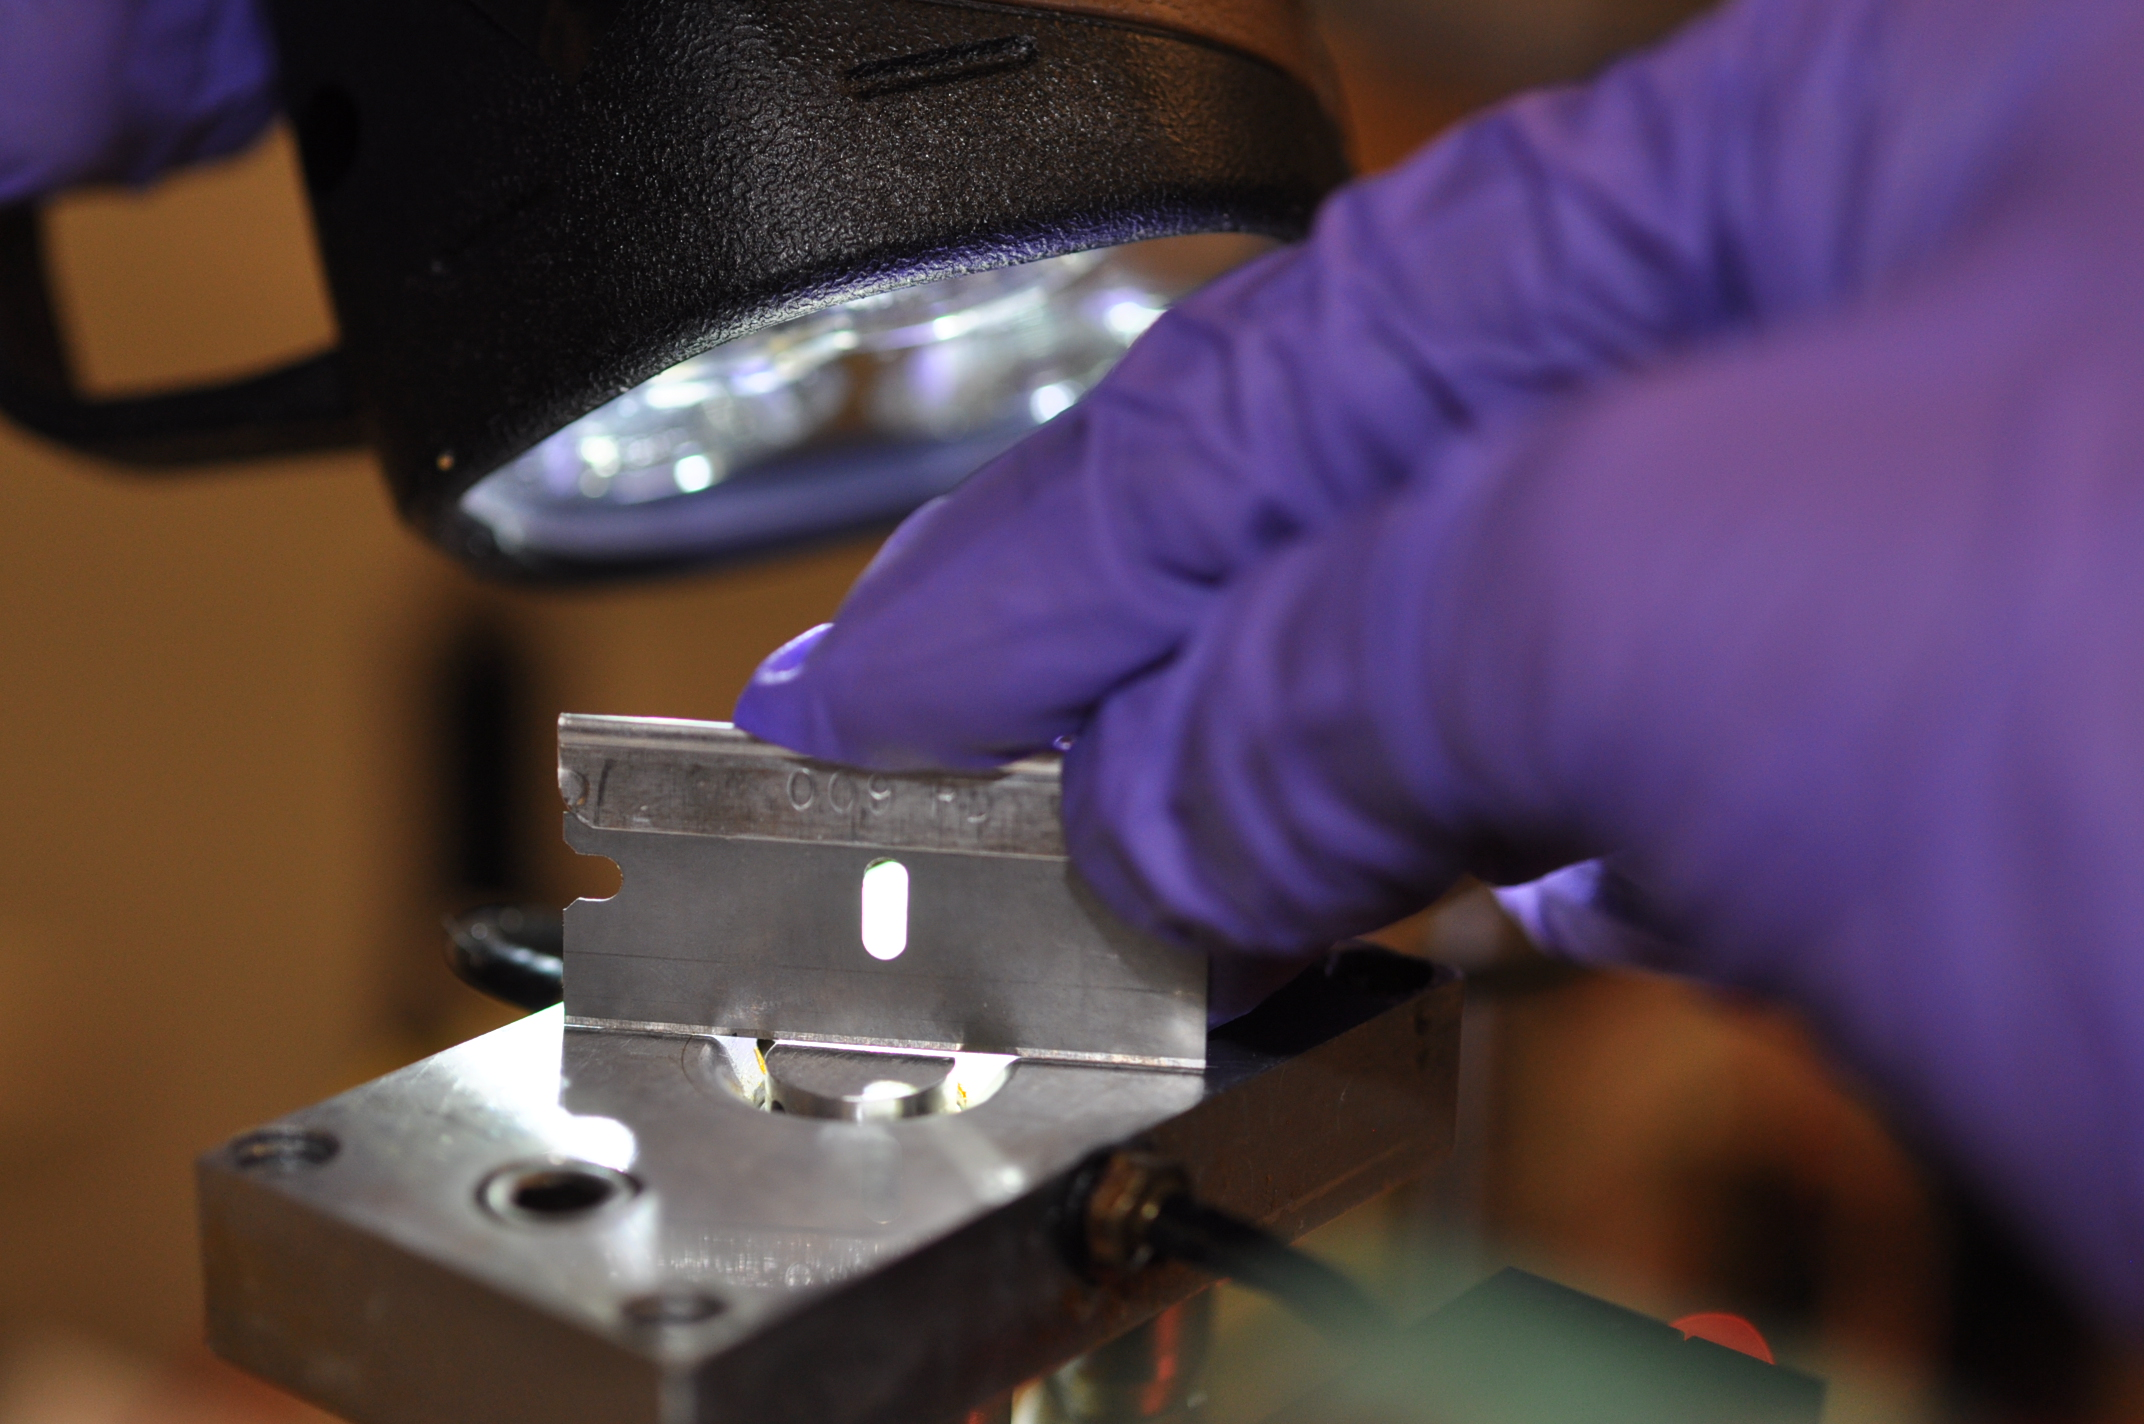
\includegraphics[width=0.3\textwidth]{shine.JPG}}
    &\raisebox{-\height}{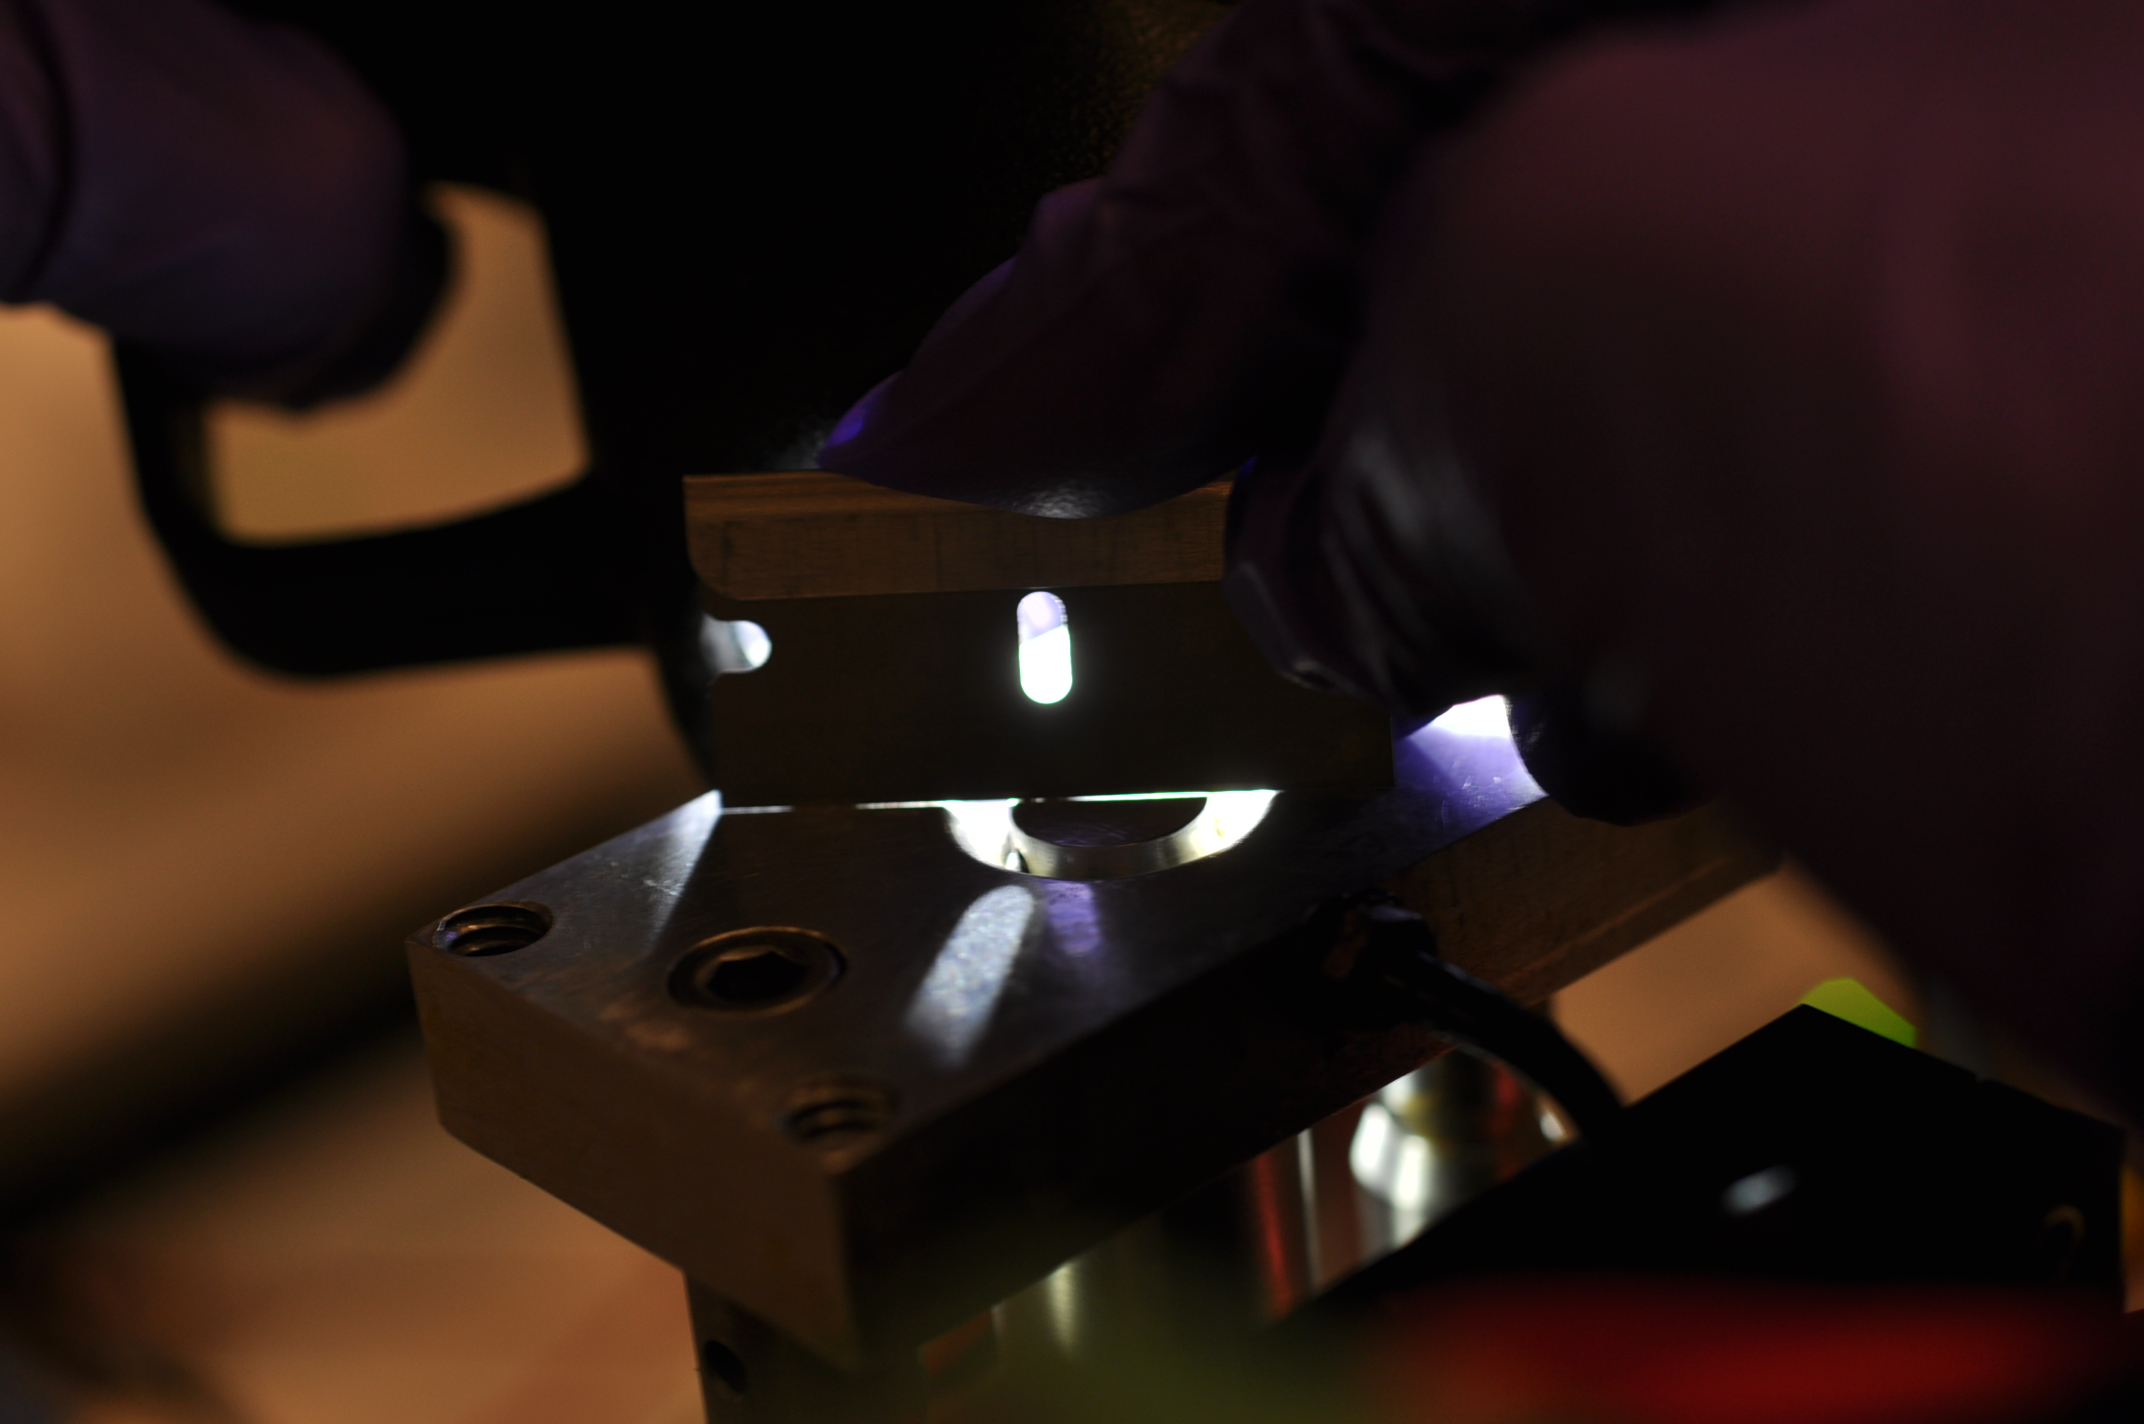
\includegraphics[width=0.3\textwidth]{exact.JPG}}
  \end{tabularx}
  
  \begin{tabularx}{\textwidth}{ XXX }
  \item \textbf{Step 8} : \textbf{Check} all the \textit{valves}. \textbf{Click} open each \textit{valve} in the interface 
    and \textbf{feel} it by hand to make sure \textit{magnetic valve} is working. You will feel a slight trembling if the 
    \textbf{magnetic valve} is popped open. If it doesn't work, see \textit{Appendix 3.2} for solution.
    &\raisebox{-\height}{\includegraphics[width=0.3\textwidth]{step8_valves.JPG}}
    &\raisebox{-\height}{\includegraphics[width=0.3\textwidth]{step8_display.JPG}}\\
  \end{tabularx}
  
  \begin{tabularx}{\textwidth}{ XXX }
  \item \textbf{Step 9} : \textbf{Clean up} the \textit{chamber} and \textbf{fix} the \textit{chamber} onto the                  stage                    through 3 screw-bonding corners.                                                                      &\raisebox{-\height}{\includegraphics[width=0.3\textwidth]{step9_cleaning.JPG}}
    &\raisebox{-\height}{\includegraphics[width=0.3\textwidth]{Step9_bonding.JPG}}\\
  \end{tabularx}
  
  \begin{tabularx}{\textwidth}{ XXX }
  \item \textbf{Step 10} : \textbf{Pour} the pre-polymer solution(\textit{see 1.3 for the recipe}) into the \textit{material 
    inlet bottle} and                 then \textbf{put} the cover with a hole on it.
    \underline{Caution: Avoid light as much as possible during the process}	     
    &\raisebox{-\height}{\includegraphics[width=0.3\textwidth]{step10_pour.JPG}}
    &\raisebox{-\height}{\includegraphics[width=0.3\textwidth]{step10_cover.JPG}}\\
  \end{tabularx}
  
  \vspace{10pt}
\end{itemize}
\subsection{Printing}\label{sec:printing}
\begin{itemize}
  \begin{tabularx}{\textwidth}{ XXX } 
  \item \textbf{Step 1} : \textbf{Open} 'runsheet.py' to create the scripts.\textbf{Set} the parameters according to your 
    printing need and \textbf{click} to                create the script files in the same folder.
    &\raisebox{-\height}{\includegraphics[width=0.3\textwidth]{step11.png}}
    &\raisebox{-\height}{\includegraphics[width=0.3\textwidth]{step12.png}}
    \\
  \end{tabularx}
  
  \begin{tabularx}{\textwidth}{ XXX } 
  \item \textbf{Step 2} : \textbf{Open} the scripts with \emph{notepad} and \textbf{double check} the parameter carefully.
    \emph{see \textbf{appendix} for the script introduction}
    &\raisebox{-\height}{\includegraphics[width=0.3\textwidth]{script21.png}}
    &\raisebox{-\height}{\includegraphics[width=0.3\textwidth]{script22.PNG}}\\
    \\
  \end{tabularx}
  
  \begin{tabularx}{\textwidth}{ XXX } 
  \item \textbf{Step 3} : \textbf{Select} the script file in the \textit{Labview} programme as well as the image folder and 
    then \textbf{click}                 refresh.
    &\raisebox{-\height}{\includegraphics[width=0.3\textwidth]{script31.png}}
    &\raisebox{-\height}{\includegraphics[width=0.3\textwidth]{script32.png}}\\
  \end{tabularx}
  
  \textbf{Now we are ready to fill the printing chamber with prepolymer solution!}
  
  \begin{tabularx}{\textwidth}{ XXX } 
  \item \textbf{Step 4} : Firstly \textbf{click} open the \textit{inlet valve} and \textit{pump}. \textbf{Wait} until there 
    are no bubbles flow through the \textit{chambers}.Secondly \textbf{close} the pump and \textbf{lower} the \textit{piston} 
    to 7mm. \textbf{Wait} about 10 seconds.  Thirdly \textbf{click} close the \textit{pump} to let the  prepolymer solution 
    flow in.
    &\raisebox{-\height}{\includegraphics[width=0.3\textwidth]{beginfilling.JPG}}
    &\raisebox{-\height}{\includegraphics[width=0.3\textwidth]{completefilling.JPG}}\\
  \end{tabularx}
  
  \begin{tabularx}{\textwidth}{ XXX } 
  \item \textbf{Step 5} : \textbf{Click} open the \textit{outlet valve} and \textbf{use} a \textit{tweezer} to \textbf{push 
    away} the bubbles into the outlet hole. \textbf{Then} \textbf{click} close the \textit{inlet valves} and \textbf{Return} 
    the Z axis to initial Z. \textbf{Wait} about 10s. Finally \textbf{Click} close the \textit{outlet valve}.\textbf{Click} to 
    begin printing.\textbf{Table \ref{table_step45} shows the valve status of material inlet procedure in Step 4 and 5}
    &\raisebox{-\height}{\includegraphics[width=0.3\textwidth]{bubbles.png}}
    &\raisebox{-\height}{\includegraphics[width=0.3\textwidth]{bubbledriving.JPG}}\\
  \end{tabularx}
  \begin{table}
    \begin{center}
      \begin{tabular}{|p{2cm} |p{2cm}|p{2cm}|p{2.5cm}|p{2cm}|p{2.5cm}|p{2cm}|}
        \hline
        \textbf{Number}&\textbf{Valve}&\textbf{1}&\textbf{2}&\textbf{3}&\textbf{4}&\textbf{5} \\ \hline
        1&\textbf{Inlet valve}&open&open&open&close&close\\     \hline
        2&\textbf{Outlet valve}&close&close&open&open&close\\
        \hline
        3&\textbf{pump}&open&close&close&close&close \\
        \hline
        4&\textbf{comment}&Accelerate the material inlet&Material fulfilling&Drive off bubbles&Return the piston to initial 
        Z&Finish material fulfilling\\
        \hline
      \end{tabular}
      \caption{Steps for material inlet procedure}\label{table_step45}
    \end{center}
  \end{table}
  
  \begin{tabularx}{\textwidth}{ XXX } 
  \item \textbf{Step 6} :\textbf{Click} print to start and \textbf{have a cup of coffee}. When the printing is done,\textbf{lift} 
    the chamber off the stage and \textbf{use} razor blade carefully to \textbf{ remove} the sample from the piston. 
    &\raisebox{-\height}{\includegraphics[width=0.3\textwidth]{lift.JPG}}
    &\raisebox{-\height}{\includegraphics[width=0.3\textwidth]{sample.JPG}}\\
  \end{tabularx}
  
  \subsection{Cleaning}       
  
  \begin{tabularx}{\textwidth}{ XXX } 
  \item \textbf{Step 1} :\textbf{Pour} Isopropyl Alchohol into the \textit{material inlet bottle} and \textbf{clean} the 
    \textbf{piston} plane. \textbf{Clean} the chamber.
    &\raisebox{-\height}{\includegraphics[width=0.3\textwidth]{Isopropyl.JPG}}
    &\raisebox{-\height}{\includegraphics[width=0.3\textwidth]{cleanstage.JPG}}\\
  \end{tabularx}
  
  \begin{tabularx}{\textwidth}{ XXX } 
  \item \textbf{Step 2}: \textbf{Fix} the \textit{Chamber} back again onto the \textit{stage plane}.\textbf{Open} \textit{inlet 
    valve},then \textit{pump}. The liquid within the chamber will gradually become lighter in color. \textbf{Close} the \textit{inlet 
    valve} and \textit{pump} when the liquid within the chamber has no color. 
    &\raisebox{-\height}{\includegraphics[width=0.3\textwidth]{completefilling.JPG}}
    &\raisebox{-\height}{\includegraphics[width=0.3\textwidth]{dilute.JPG}}\\
  \end{tabularx}\\

  \begin{figure}
    \centering
    \includegraphics[width=\textwidth]{con1.png}
  \end{figure}
  
  \begin{tabularx}{\textwidth}{ XXX } 
  \item \textbf{Step 3}:  \textbf{Reconnect} the \textit{pump} to the \textit{outlet valve} before \textbf{opening} \textit{inlet, 
    outlet valve} and \textit{pump}.\textbf{Wait} until all Isopropyl Alchohol is pumped out.
    &\raisebox{-\height}{\includegraphics[width=0.3\textwidth]{disconnect.JPG}}
    &\raisebox{-\height}{\includegraphics[width=0.3\textwidth]{connect.JPG}}\\
  \end{tabularx}

  \begin{figure}
    \centering
    \includegraphics[width=\textwidth]{con2.png}
  \end{figure}
  
  \begin{tabularx}{\textwidth}{ XXX } 
  \item \textbf{Step 4}:\textbf{Reinstate} the connection in step 2 and \textbf{put} the tubes of \textit{outlet valve,pump}
    into the waste bottle. \textit{Remove} the chamber and \textbf{clean it up}. \textbf{Adjust} the \textit{piston} to 
    \textbf{3mm} and in order to completely clean it. \textbf{Return} the piston back to \textbf{7mm}.  
    &\raisebox{-\height}{\includegraphics[width=0.3\textwidth]{chamber.JPG}}
    &\raisebox{-\height}{\includegraphics[width=0.3\textwidth]{stagewipe.JPG}}\\
  \end{tabularx}
  
  \begin{tabularx}{\textwidth}{ XXX } 
  \item \textbf{Step 5}: \textbf{Close} the \textit{projector, powersupply, computer} before \textbf{turning off} the 
    \textit{powerstrip}. \textbf{Pour} the residue in the \textit{waste bottle} into the \textit{waste tank}
    &\raisebox{-\height}{\includegraphics[width=0.3\textwidth]{mainoverview.JPG}}
    &\raisebox{-\height}{\includegraphics[width=0.3\textwidth]{waste2.PNG}}\\
  \end{tabularx}
  
\end{itemize}

\pagebreak


\appendix
\section{\textit{Appendix}}\label{sec:Appendix}
\begin{itemize}
  \subsection{Razor blade method to determine the printing plane(initial Z)}
  \begin{tabularx}{\textwidth}{XXX}
    1: \textbf{Press} the \textit{blade edge} to the stage plane which is at 7mm in z direction.\textbf{Elevate} the                 piston to 6mm(the default printing position). 
    &\raisebox{-\height}{\includegraphics[width=0.3\textwidth]{printingplane.JPG}}
    &\raisebox{-\height}{\includegraphics[width=0.3\textwidth]{blade1.png}}
  \end{tabularx}
  
  \begin{tabularx}{\textwidth}{XXX}
    2:\textbf{Shine} the interface between the blade and the stage plane from behind using a \textit{torch} and \textbf{observe}                 directly from the front.
    &\raisebox{-\height}{\includegraphics[width=0.3\textwidth]{shine.JPG}}
    &\raisebox{-\height}{\includegraphics[width=0.3\textwidth]{blade2.png}}
  \end{tabularx}
  
  
  \begin{tabularx}{\textwidth}{XXX}
  \item If there is continuous light leaking from \textit{piston-blade interface} while there is no light leaking from 
    \textit{stage-blade interface}, it indicates that the piston is \textbf{too low} in Z position(\textit{the number is too big}).                      \textbf{Lower} the \textit{piston} to 7mm and \textbf{elevate} it back again to 5.9mm.
    &\raisebox{-\height}{\includegraphics[width=0.3\textwidth]{toolow.JPG}}
    &\raisebox{-\height}{\includegraphics[width=0.3\textwidth]{blade3.png}}
  \end{tabularx}
  \begin{tabularx}{\textwidth}{XXX}
  \item If there is no light leaking from \textit{piston-blade interface} while you observe continuous light at \textit{stage-blade 
    interface}, it indicates that the piston is \textbf{too high} in Z position(\textit{the number is too small}). \textbf{Lower}                    the \textit{piston} to 7mm and \textbf{elevate} it back again to 6.1mm.
    &\raisebox{-\height}{\includegraphics[width=0.3\textwidth]{toohigh.JPG}}
    &\raisebox{-\height}{\includegraphics[width=0.3\textwidth]{blade4.png}}
  \end{tabularx}
  \begin{tabularx}{\textwidth}{XXX}
  \item \textbf{Repeat} the lower/elevate cycle until no light leakage is observed from both \textit{stage-blade and piston-blade} 
    interface. \emph{\textbf{Set} the current Z positon as the \textbf{initial Z}. }
    &\raisebox{-\height}{\includegraphics[width=0.3\textwidth]{exact.JPG}}
    &\raisebox{-\height}{\includegraphics[width=0.3\textwidth]{blade5.png}}
  \end{tabularx}
  \subsection{Maintainece}
  \subsubsection{Elevate the voltage supply to open the valve}

  \begin{tabularx}{\textwidth}{XXX}
    If the valve doesn't work when the voltage supply is 9V, \textbf{Try} elevate the voltage manually to 10-12V. \textbf{Feel} 
    it by hand whether the magnetic valve is popped open under higher voltage. \textbf{Never} elevate the voltage beyond 12V. 
    It will cause permanent damage to the valve.
    &\raisebox{-\height}{\includegraphics[width=0.3\textwidth]{step5_2.JPG}}
    &\raisebox{-\height}{\includegraphics[width=0.3\textwidth]{step8_valves.JPG}}
  \end{tabularx}

  \subsubsection{Adjust the focal length of the projected image}
  \begin{tabularx}{\textwidth}{ XXX }
    \textbf{Change} the focal length by rotating the focusing ring of the \textit{reduction lens} until the precision of the 
    projected image reaches its best.
    &\raisebox{-\height}{\includegraphics[width=0.3\textwidth]{reduction2.jpeg}}
    &\raisebox{-\height}{\includegraphics[width=0.3\textwidth]{overview.png}}
    \\
  \end{tabularx}

  \clearpage
  \subsection{Materials}
  \subsubsection{\textit{PEGDA SYSTEM}}
  \textbf{Features}:\\
  (1)The most mature system for hydrogel printing.\\
  (2)The printed hydrogel is hardest and most brittle among three material systems listed.  \\
  (3)It exhibits almost no elasticity. \\
  (4)Its volume swelling ratio in water is 120\%.\\
  \begin{table}
    \begin{center}
      \begin{tabular}{ | c | c | c | c | c |}
        \hline
        \textbf{name}&\textbf{content}&\textbf{company}&\textbf{catalog number}&\textbf{comments} \\ 
        \hline
        Poly(ethylene glycol) diacrylate(Mw~575)&98\%&Sigma-Aldrich&437442&Hydrogel backbone \\     
        \hline
        phenylbis(2,4,6-trimethylbenzoyl) phosphine oxide&2\%&Sigma-Aldrich&511447&photo-initiator(PI) \\
        \hline
        Sudan I&0.1\%&Sigma-Aldrich&103624&photo-absorber \\
        \hline
      \end{tabular}
      \caption{PEGDA SYSTEM RECIPE}
    \end{center}
  \end{table}

  \subsubsection{\textit{PEG/PEGDA SYSTEM}}
  \textbf{Features}:\\
  (1):This system is basically employed in the printing the backbone of bio-materials due to the bio-compatibility and 
  hydro-philicity of PEG.(Peptides or cells can be grafted onto PEG, thus fabricating a soft biological scaffold with 
  unlimited potential.)\\
  (2)The PEG/PEGDA system hydrogel is softer than PEGDA system but much harder than NIPAM/Sodium acrylate/PEGDA system.\\
  (3)The PEG/PEGDA system hydrogel has around 10-20\% elongation before rupture.\\
  (4) It exhibits around 160\% volume expansion ratio in the water.\\
  (5) It can be bonded very well with PEGDA hydrogels.
  \begin{table}
    \begin{center}
      \begin{tabular}{ | c | c | c | c | c |}
        \hline
        \textbf{name}&\textbf{content}&\textbf{company}&\textbf{catalog number}&\textbf{comments} \\ 
        \hline
        Poly(ethylene glycol) diacrylate(Mw~575)&33\%&Sigma-Aldrich&437442&Hydrogel backbone \\     
        \hline
        Poly(ethylene glycol)(Mw~200)&66\%&Sigma-Aldrich&1546401&Pore generator \\      
        \hline
        phenylbis(2,4,6-trimethylbenzoyl) phosphine oxide&0.67\%&Sigma-Aldrich&511447&photo-initiator(PI) \\
        \hline
        Sudan I&0.1\%&Sigma-Aldrich&103624&photo-absorber \\
        \hline
      \end{tabular}
      \caption{PEG/PEGDA SYSTEM RECIPE}
    \end{center}
  \end{table}
  \subsubsection{\textit{NIPAM/Sodium Acrylate/PEGDA Hydrogel SYSTEM}}
  \textbf{Features}:\\
  (1)This system features the extremely high swelling ratio in water.In our current recipe, PEGDA:MONOMERS(NIPAM:SODIUM 
  ACRYLATE) is 1:5 by weight and 330\% volume expansion can be achieved in water.\\
  (2)By tuning the weight ratio of PEGDA to monomers, different volume expansion ranging from 200\% to 800\% can be 
  realized.The correlation between the volume expansion and the PEGDA/MONOMER weight ratio is illustrated in the 
  picture below.\\
  (3)Hydrogels in this system is the softest among the three material systems listed.
  (4)Hydrogels in this system enjoys 30-40\% elongation before rupture.
  (5)Hydrogels in this system cannot be bonded very well with the PEGDA hydrogels.
  \begin{figure}
    \centering
    \includegraphics[width=400pt]{graph.png}
    \caption{The volume expansion ratio of the hydrogels with different propotion of PEGDA}
  \end{figure}
  \\


  \begin{table}
    \begin{center}
      \begin{tabular}{ |p{5cm}| c | c | c | c |}
        \hline
        \textbf{name}&\textbf{content}&\textbf{company}&\textbf{catalog number}&\textbf{comments} \\ 
        \hline
        Poly(ethylene glycol) diacrylate(Mw~575)&7.7\%&Sigma-Aldrich&437442& Hydrogel backbone\\     
        \hline
        Sodium acrylate&25.7\%&Sigma-Aldrich&408220&To increase swelling ratio\\ 
        \hline
        N-Isopropylacrylamide&5.1\%&Sigma-Aldrich&415324&To increase the toughness.\\ 
        \hline
        phenylbis(2,4,6-trimethylbenzoyl) phosphine oxide&0.154\%&Sigma-Aldrich&511447&photo-initiator(PI)\\
        \hline
        Isopropyl alcohol&9.9\%&Sigma-Aldrich&W292907&To dissolve PI\\      
        \hline
        Sudan I&0.1\%&Sigma-Aldrich&103624&photo-absorber \\
        \hline
      \end{tabular}
      \caption{Nipam/Sodium acrylate/PEGDA SYSTEM RECIPE}
    \end{center}
  \end{table}
  \pagebreak
  \subsection{Hydrogels preparation: Pre-printing test of the material}
  \textit{\textit{Swellable} Sodium Acrylate/NIPAM/PEGDA system}\\
  Generally in a hydrogel system, its free-swelling ratio in the water is \textbf{positively} correlated with the ionic 
  concentration. \textit{In a material point of view}, using monomers with ionic property(Such as Sodium Acrylate or 
  acrylic acid) can greatly increase the free-swelling ratio of the hydrogels in water. It is largely because that the 
  ions can lower the chemical-potential within the hydrogel system thus creating the chemical gradient for the surrounding 
  water to flow in. If you want to test the swelling performance of the hydrogels before 3d-printing, following the steps 
  below:
  
  
  \begin{tabularx}{\textwidth}{XXX}
  \item \textbf{Solution preparation}: Sodium acrylate:NIPAM:DI water=1:1:5 by weight solution was \textbf{prepared} 
    after 20-min vigorous stirring. \textbf{Stir} the PEGDA:photo-initiator=49:1 mixture in a light-proof brown bottle 
    for 2-3h. \textbf{Make sure} there are no visible green particles interspersed in the PEGDA:PI mixture. 
    &\raisebox{-\height}{\includegraphics[width=0.3\textwidth]{sp1.jpeg}}
    &\raisebox{-\height}{\includegraphics[width=0.3\textwidth]{sp2.jpeg}}
  \end{tabularx}
  
  \begin{tabularx}{\textwidth}{XXX}
  \item \textbf{Mold preparation}:\textbf{Stick} the \textit{plastic mold} onto the \textit{teflone plate} \textbf{using} 
    \textit{3M-Scotch}.
    &\raisebox{-\height}{\includegraphics[width=0.3\textwidth]{mp1.jpeg}}
    &\raisebox{-\height}{\includegraphics[width=0.3\textwidth]{mp2.jpeg}}
  \end{tabularx}
  
  \begin{tabularx}{\textwidth}{XXX}
  \item \textbf{UV-LAMP preparation}:\textbf{Hang} the UV-Lamp on two vertically placed \textit{Acrylic box}. \textbf{Put} 
    the \textit{Teflone plate} with \textit{plastic mold} on it right under the \textit{UV-LAMP}.
    &\raisebox{-\height}{\includegraphics[width=0.3\textwidth]{uvp1.jpeg}}
    &\raisebox{-\height}{\includegraphics[width=0.3\textwidth]{uvp2.jpeg}}
  \end{tabularx}
  
  
  \begin{tabularx}{\textwidth}{XXX}
  \item \textbf{Syringe blending}:Two \textit{Luer-lok syringes} were \textbf{used} in this step together with a 
    \textit{connector} to ensure the oxygen-free and homogeneous blending of the pre-polymer solution. \textbf{Draw} 
    certain amount of Sodium acrylate/NIPAM solution into one \textit{syringe} and PEGDA/PI mixture into another. 
    \footnote{the amount of two should be calculated according to the PEGDA/monomer(NIPAM:sodium acrylate ratio) you need} 
    Carefully \textbf{push} the air out of both \textit{syringes} and \textbf{use} \textit{connectors} to vertically bond 
    them. Then begin \textbf{mixing}.
    &\raisebox{-\height}{\includegraphics[width=0.3\textwidth]{sb1.jpeg}}
    &\raisebox{-\height}{\includegraphics[width=0.3\textwidth]{sb2.jpeg}}
  \end{tabularx}

  \begin{tabularx}{\textwidth}{XXX}
  \item \textbf{UV-curing}:\textbf{Push} the mixed solution into one syringe and Quick \textbf{transfer} it into the mold. 
    \textbf{Cover} the \textit{mold} with \textit{micro-slides}.Carefully  \textbf{Set} up plastic boards around the UV-Lamp 
    to prevent UV-light leakage.\textbf{Shine} the pre-polymer solution in the textit{mold} \textbf{using} 365nm wavelength 
    \footnote{365nm is the peak adsorption wavelength of the PI in our system}. 
    &\raisebox{-\height}{\includegraphics[width=0.3\textwidth]{uvc1.jpeg}}
    &\raisebox{-\height}{\includegraphics[width=0.3\textwidth]{uvc2.jpeg}}
  \end{tabularx}
  
  \begin{tabularx}{\textwidth}{XXX}
  \item \textbf{Hydrogel swelling test}:\textbf{Turn off} the \textit{UV-LAMP} and \textbf{Remove} the cured sample from 
    the \textit{mold} \textbf{using} a \textbf{razer-blade}. \textbf{measure} the initial weight of the sample on the 
    \textit{balance} and \textbf{put} it directly into a \textit{beaker} with water.\footnote{the initial volume of the 
      sample is determined by the mold you use}.After 12 h, \textbf{Take} the sample out and \textbf{wipe} the water on the 
    surface. \textbf{Measure} the weight and volume of the hydrogels in swollen state individually using a \textit{balance} 
    and a \textit{vernier scale}.
    &\raisebox{-\height}{\includegraphics[width=0.3\textwidth]{swell1.jpeg}}
    &\raisebox{-\height}{\includegraphics[width=0.3\textwidth]{swell2.jpeg}}
  \end{tabularx}
  


  \begin{tabularx}{\textwidth}{XXX}        
  \item \textbf{Cleaning}: \textbf{Wash} the \textit{plastic mold} with \textit{acetone} and \textbf{scratch off} the 
    \textit{scotch} residue \textbf{using} a \textit{blade}. Then \textbf{wash} the \textit{mold} again using water. 
    \textit{Teflone plate} should also be \textbf{wahsed} with water to \textbf{wipe off} the residue on its surface.
    If you want to test the bonding of two hydrogels with different recipes, you should prepare the \textit{solution A 
    and B, mold and UV-LAMP} as stated before. However in the UV-curing section, \textbf{Do not use a slide to cover the 
     mold}.\textbf{Use} a \textit{pippete} to \textbf{add} a layer of solution A and shine immediately with \textit{UV-Lamp} 
    to \textbf{cure} it. After \textbf{curing} several layers of solution A hydrogels, \textbf{repeat} the previous steps 
    and \textbf{cure} another few layers of solution B hydrogels.\textbf{Remove} the sample from the \textit{mold} carefully 
    to see if they can be bonded together. 
    &\raisebox{-\height}{\includegraphics[width=0.3\textwidth]{bond1.jpeg}}
    &\raisebox{-\height}{\includegraphics[width=0.3\textwidth]{bond2.jpeg}}
  \end{tabularx}
  

  
\end{itemize}



\end{document}
